% !TEX program = lualatex
% Tema 1: mismo contenido que la versión anterior (originales/Tema1_main_original.tex);
% sólo cambia el formato. El cuerpo está en Tema1_cuerpo.tex.
\documentclass[11pt,twoside]{article}
\usepackage{apuntes-oscuro}
\usepackage{float,centernot,multirow,subcaption}
\usetikzlibrary{3d,patterns,shadings,angles,quotes,matrix,bending,decorations.markings}

\asignatura{Ecuaciones Diferenciales}
\cabecera{Tema 1\ \ ·\ \ EDO de primer orden}
\hypersetup{pdftitle={Tema 1. Ecuaciones diferenciales de primer orden},pdfauthor={Daniel Martín Guerrero}}

% ---------- notación del documento original ----------
\renewcommand{\Id}{\mathrm{Id}}
\DeclareMathOperator{\Hom}{Hom}
\counterwithout{figure}{section}

% ---------- numeración original: un contador por tipo de entorno ----------
\makeatletter
\@for\@tipo:={definicion,ejemplo,ejercicio,observacion,proposicion,corolario,teorema,lema}\do{%
  \newcounter{c@@\@tipo}[section]}
\newcommand\@numtipo[1]{\stepcounter{c@@#1}\xdef\@numfijo{\thesection.\arabic{c@@#1}}}
\@for\@tipo:={definicion,ejemplo,ejercicio,observacion,proposicion,corolario,teorema,lema}\do{%
  \edef\@tmp{\noexpand\AddToHook{env/\@tipo/before}{\noexpand\@numtipo{\@tipo}}}\@tmp}
% Ejercicio (etiqueta dorada en línea, texto recto)
\NewDocumentEnvironment{ejercicio}{O{}}
  {\par\addvspace{10pt}\Needspace{6\baselineskip}\refstepcounter{entorno}\noindent
   {\color{gold}\bfseries Ejercicio~\theentorno}%
   \if\relax\detokenize{#1}\relax\else\ \textcolor{muted}{(#1)}\fi\textcolor{gold}{.}\ \ignorespaces}
  {\par\addvspace{4pt}}
\AddToHook{env/ejercicio/end}{\global\let\@numfijo\relax}
\makeatother

% ---------- cajas del documento original, en el estilo oscuro ----------
\tcbset{
  caja_ejercicio/.style={baseoscuro,colframe=acc,boxed title style={colframe=acc},
    title={\textcolor{acc}{\textsc{Resolución}}}},
  recuadro/.style={enhanced,breakable,colback=boxbg,coltext=fg,frame hidden,
    borderline west={2.2pt}{0pt}{lav},arc=0pt,left=10pt,right=10pt,top=7pt,bottom=7pt,
    before skip=12pt,after skip=12pt,
    before upper={\textcolor{lav}{\textsc{#1}}\par\vspace{4pt}}},
}
\pgfplotsset{t1/.style={oscuro,axis lines=left,
  every axis x label/.style={at={(axis description cs:1.0,0)},anchor=west,xshift=5pt},
  every axis y label/.style={at={(axis description cs:0,1.0)},anchor=south,yshift=3pt},samples=200},
  t1c/.style={t1,extra x ticks={0},extra y ticks={0},extra x tick labels={},extra y tick labels={},
  extra tick style={grid=major,major grid style={rulec,line width=0.4pt},major tick length=0pt}}}
\newcommand\leyenda[2]{\textcolor{#1}{\rule[2.2pt]{11pt}{1.1pt}}\ #2}
\newcommand\leyendad[2]{\textcolor{#1}{\rule[2.2pt]{3.5pt}{1.1pt}\,\rule[2.2pt]{3.5pt}{1.1pt}}\ #2}

\begin{document}

% =====================================================================
%  PORTADA
% =====================================================================
\begin{titlepage}
\thispagestyle{empty}
\centering
\vspace*{-0.6cm}

\includegraphics[width=4.6cm]{figuras/usal.png}\par
\vspace{0.75cm}
{\color{sky}\rule{\textwidth}{0.5pt}}\par
\vspace{0.55cm}
{\color{muted}\small\textls[220]{\textsc{Facultad de Ciencias}}\quad·\quad\textls[220]{\textsc{Grado en Física}}}\par
\vspace{1.25cm}
{\color{acc}\textls[260]{\textsc{Ecuaciones Diferenciales}}}\par
\vspace{0.2cm}
{\color{muted}\small\textls[260]{\textsc{Tema 1}}}\par
\vspace{1.25cm}
{\fontsize{27}{33}\selectfont\bfseries Ecuaciones diferenciales\par}
\vspace{0.12cm}
{\fontsize{19}{24}\selectfont\bfseries de primer orden\par}
\vspace{0.55cm}
{\color{acc}\rule{2.4cm}{0.8pt}}\par
\vspace{0.45cm}
{\color{muted}\small\itshape Familias de curvas y envolventes\quad·\quad Campo de direcciones\quad·\quad Separables y lineales\par
Bernoulli y Riccati\quad·\quad Pfaff y factor integrante\quad·\quad Lagrange y Clairaut\par}
\vspace{0.45cm}
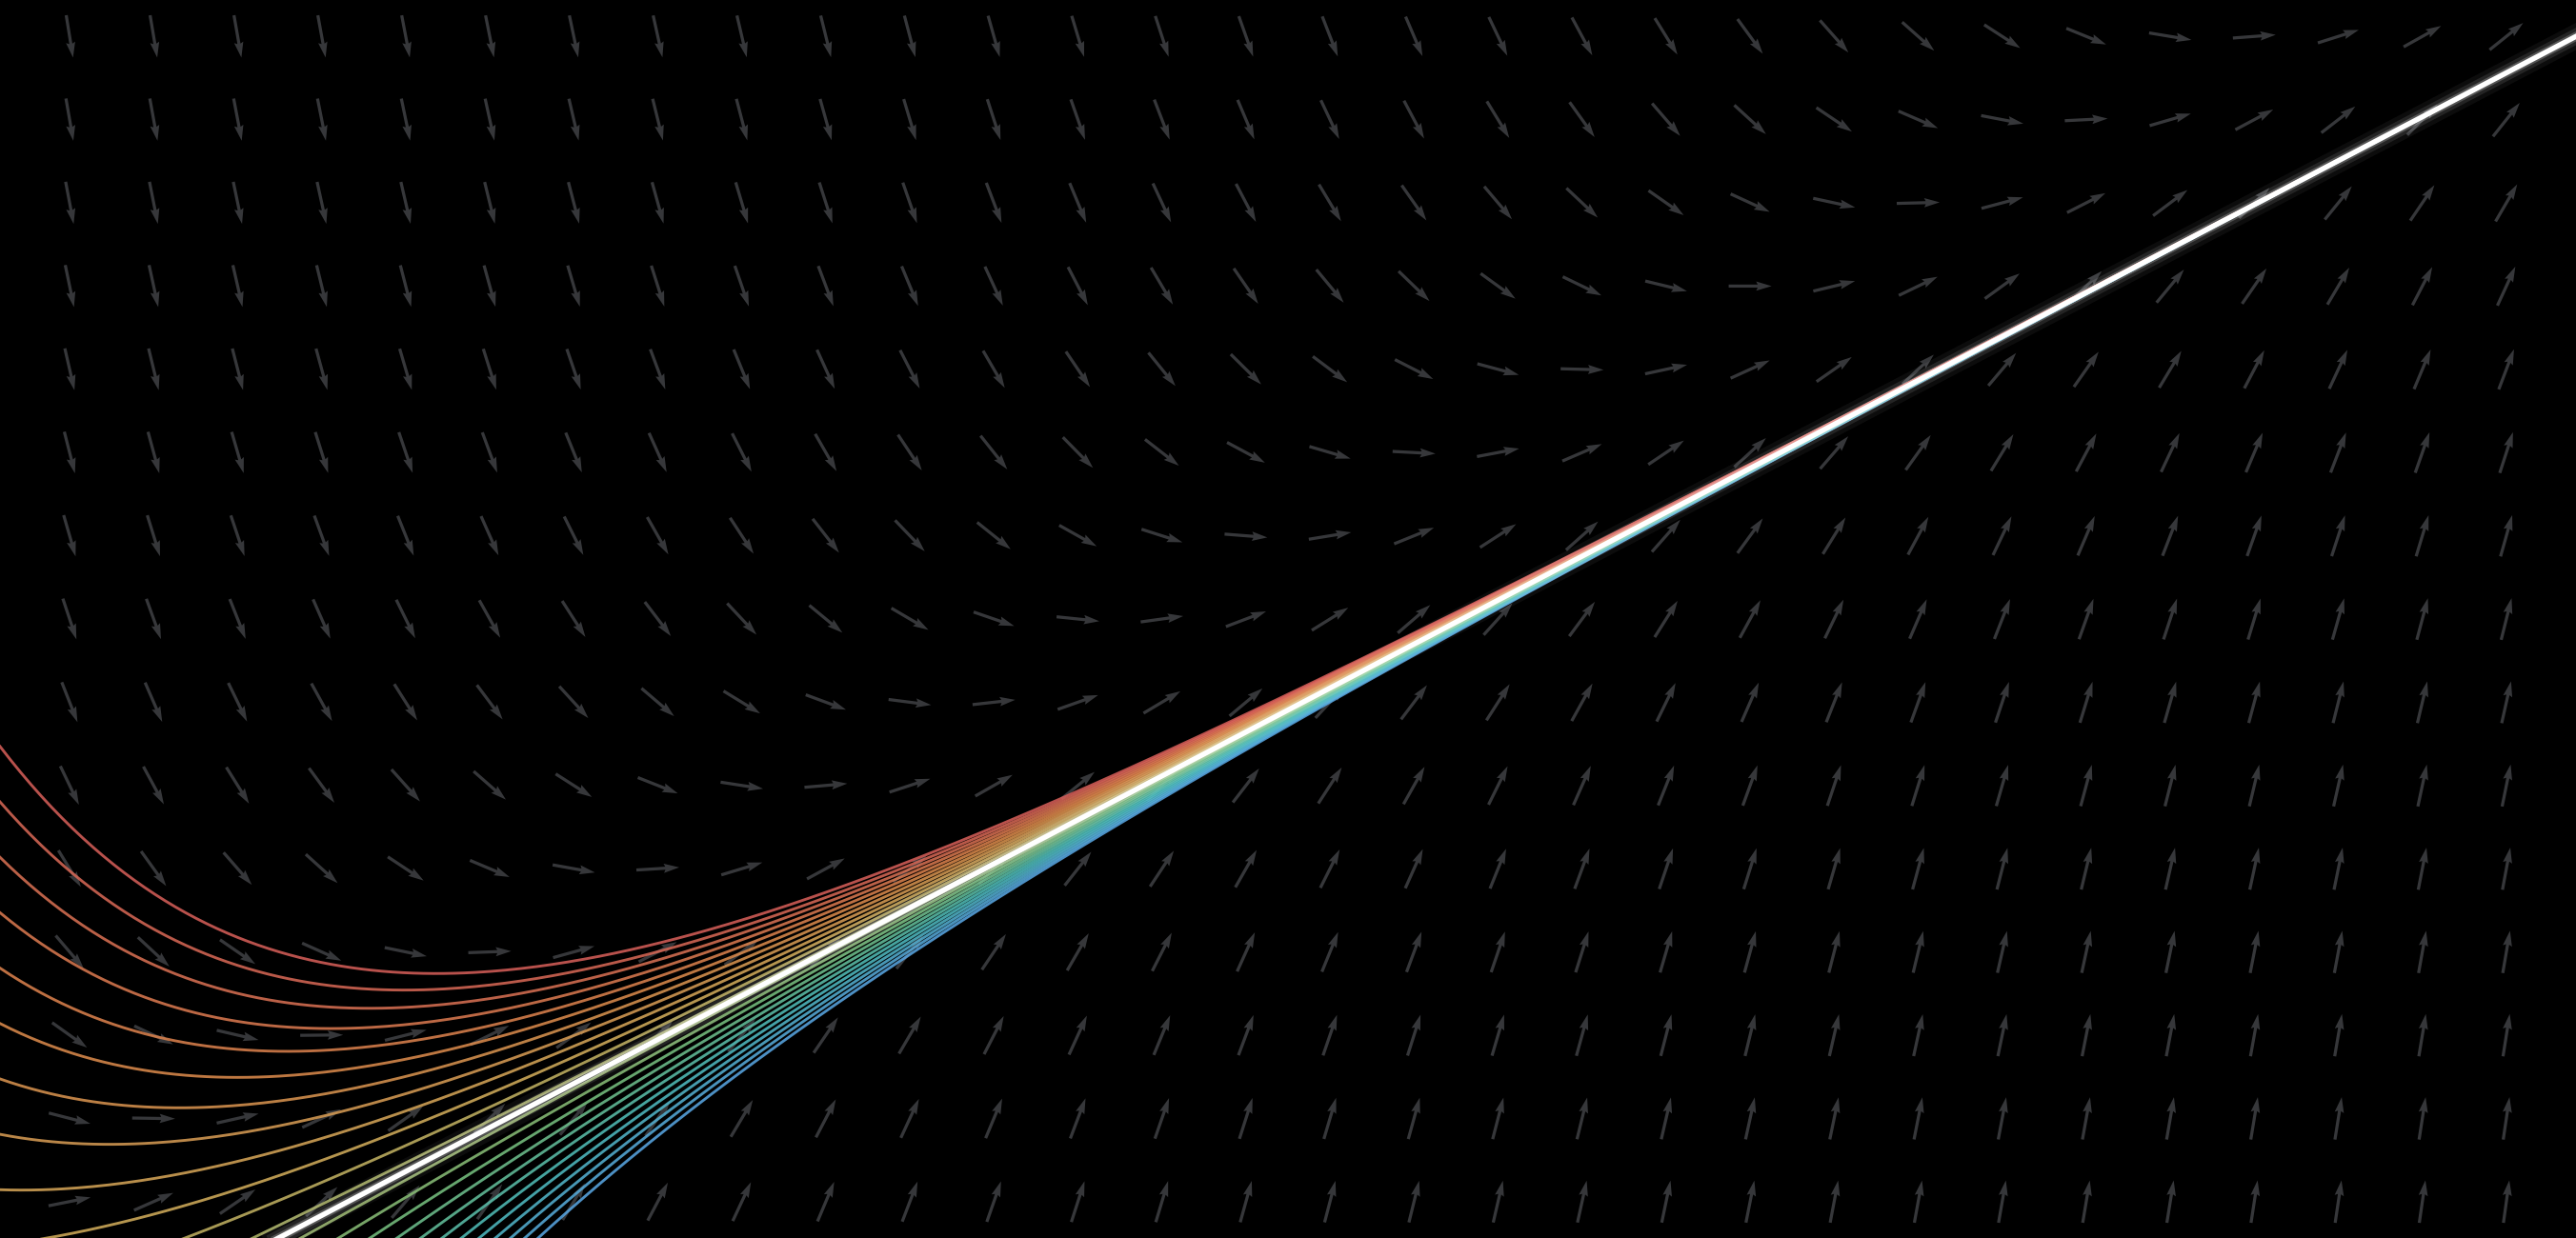
\includegraphics[width=0.86\textwidth]{figuras/portada_t1.png}\par
\vspace{0.35cm}
{\small$\displaystyle y'=f(x,y),\qquad y(x_0)=y_0\qquad\Longrightarrow\qquad y=\varphi(x,C)$\par}
\vfill
{\color{sky}\rule{\textwidth}{0.5pt}}\par
\vspace{0.3cm}
\begin{minipage}[t]{0.32\textwidth}\raggedright
{\color{acc}\footnotesize\textls[200]{\textsc{Autor}}}\par\vspace{2pt}
{\small Daniel Martín Guerrero}
\end{minipage}\hfill
\begin{minipage}[t]{0.32\textwidth}\centering
{\color{acc}\footnotesize\textls[200]{\textsc{Profesorado}}}\par\vspace{2pt}
{\small Pilar García Estévez\\ José Beltrán Jiménez\\ María Pérez Garrote}
\end{minipage}\hfill
\begin{minipage}[t]{0.32\textwidth}\raggedleft
{\color{acc}\footnotesize\textls[200]{\textsc{Apuntes formalizados}}}\par\vspace{2pt}
{\small Salamanca, curso 2026/2027}\\[1pt]
{\footnotesize\color{muted}Teoría y seminarios resueltos}
\end{minipage}
\end{titlepage}

\setcounter{page}{2}
{\hypersetup{linkcolor=fg}\tableofcontents}
\clearpage

\section{Consideraciones generales}

\subsection{Fenomenología y breve historia}

El desarrollo analítico de las ecuaciones diferenciales ordinarias está intrínsecamente ligado a la evolución de la física y las matemáticas a lo largo de los siglos. Las bases fundacionales fueron establecidas por Newton (1642) mediante el desarrollo del cálculo diferencial, y por Leibniz (1646), Huygens (1529) y los hermanos Bernoulli con el estudio de problemas clásicos como la catenaria, el péndulo y la cuerda vibrante.

A lo largo del desarrollo científico, se hizo patente la importancia de los sistemas no lineales, los cuales marcan los límites de la predicción científica clásica. Problemas fundamentales, como el de los tres cuerpos abordado por Poincaré (1854) y el análisis del sólido rígido por Kovalevskaya (1850), revelaron la profunda complejidad oculta tras formulaciones aparentemente simples. 

Esta línea de investigación condujo al descubrimiento de los sistemas críticos y del caos determinista. En estos sistemas (cuyo ejemplo paradigmático son los modelos de predicción meteorológica), conocemos rigurosamente las leyes que los gobiernan, pero su extrema sensibilidad a las condiciones iniciales —fenómeno conocido popularmente como \textit{efecto mariposa}— nos impide predecir su comportamiento a largo plazo. Un análogo geométrico de esta sensibilidad se observa en el diagrama del billar de Sinaí, donde la incrustación de una columna en el centro del recinto provoca que variaciones del $5\%$ o $10\%$ en el ángulo de incidencia generen trayectorias radicalmente divergentes.

En el ámbito de la dinámica de fluidos y la propagación de ondas, la no linealidad origina fenómenos extraordinarios como los solitones. Un solitón es una onda localizada que se propaga manteniendo aproximadamente su forma gracias a un equilibrio dinámico perfecto entre los efectos de dispersión y la no linealidad. El ejemplo matemático paradigmático es la ecuación de Korteweg-de Vries (KdV): $u_t + 6uu_x + u_{xxx} = 0$, la cual admite soluciones del tipo $u(x,t) = \frac{c}{2} \text{sech}^2\left[ \frac{\sqrt{c}}{2}(x - ct - x_0) \right]$, demostrando cómo la forma de la onda subsiste inalterada mientras se desplaza con velocidad $c$.

Físicamente, los tsunamis constituyen un análogo natural de estas ondas solitarias. En aguas profundas, las ondas superficiales se comportan como ondas lineales comunes; no obstante, en aguas poco profundas (donde la profundidad $h$ es pequeña respecto a la longitud de onda), emerge el régimen de aguas someras. Esta dinámica se modela mediante las ecuaciones no lineales de Saint-Venant:
\begin{align*}
    \frac{\partial h}{\partial t} + \frac{\partial (hu)}{\partial x} &= 0 \\
    \frac{\partial u}{\partial t} + u \frac{\partial u}{\partial x} + g \frac{\partial h}{\partial x} &= 0
\end{align*}
donde $h(x,t)$ denota la profundidad local y $u(x,t)$ la velocidad horizontal del fluido. Bajo este régimen, la velocidad de fase se aproxima por $c \simeq \sqrt{gh}$ y, al acercarse a la costa (fenómeno de \textit{shoaling}), la disminución de $h$ provoca que la energía se concentre drásticamente, incrementando la amplitud destructiva de la ola.

\subsection{Algunas notaciones}

Para establecer un lenguaje matemático coherente, emplearemos las notaciones clásicas del cálculo diferencial y vectorial establecidas por figuras como Cayley (1821).
Para una función de una variable independiente, utilizaremos primordialmente:
$$ y = y(x), \quad y'(x) = \frac{dy}{dx}, \quad y''(x) = \frac{d^2y}{dx^2} $$
Si la variable independiente representa el tiempo ($t$), es frecuente adoptar la notación de Newton:
$$ x = x(t), \quad \dot{x} = \frac{dx}{dt}, \quad \ddot{x} = \frac{d^2x}{dt^2} $$
Para funciones de múltiples variables, como $u = u(x,y)$, la notación de derivadas parciales se simplifica mediante subíndices:
$$ u_x = \frac{\partial u}{\partial x}, \quad u_y = \frac{\partial u}{\partial y}, \quad u_{xx} = \frac{\partial^2 u}{\partial x^2}, \quad u_{xy} = \frac{\partial^2 u}{\partial x \partial y} $$

\subsection{Repaso del concepto de derivada y de diferencial}

\textbf{Nota importante:} Es imperativo no confundir nunca el concepto de derivada con el de diferencial. La derivada, definida clásicamente mediante el límite del cociente incremental:
$$ y'(x) = \lim_{\Delta x \to 0} \frac{y(x + \Delta x) - y(x)}{\Delta x} = \tan \alpha $$
constituye una función finita que describe la pendiente de la recta tangente en un punto.

Por otro lado, la diferenciabilidad de una función $f: \mathbb{R} \to \mathbb{R}$ en un punto $a$ se entiende analíticamente como una \textbf{aproximación lineal local}. Expresamos el incremento de la función $\Delta y$ ante una perturbación $\Delta x$ como:
$$ \Delta y = f(a + \Delta x) - f(a) = f'(a)\Delta x + o(\Delta x) $$
donde $o(\Delta x)$ es la notación de Landau para un infinitésimo de orden superior, es decir, un error topológico que decae a cero más rápidamente que la propia perturbación, cumpliendo $\lim_{\Delta x \to 0} \frac{o(\Delta x)}{\Delta x} = 0$. 

La diferencial, por tanto, es una cantidad infinitesimal vinculada linealmente al incremento de la variable independiente. Ambas magnitudes (derivada y diferencial) se relacionan íntimamente mediante la expresión:
$$ dy = y'(x) dx $$

Para funciones de varias variables, por ejemplo $z = z(x,y)$, la diferencial total captura la aproximación lineal en todas las dimensiones del dominio, definiéndose como:
$$ dz = z_x dx + z_y dy $$
donde $z_x$ y $z_y$ son las derivadas parciales de $z(x,y)$ con respecto a $x$ e $y$ respectivamente. Geométricamente, una curva plana puede presentarse en diversas formas topológicas:

\begin{itemize}
    \item \textbf{Forma intrínseca}: Una curva en el plano puede describirse por $y = y(x)$. La pendiente de la curva en cada punto viene descrita por la derivada en el punto:
    $$ \tan \alpha = y'(x) $$
    
    \item \textbf{Curva en coordenadas paramétricas}: Una curva en el plano puede darse también en coordenadas paramétricas dependiendo de un escalar $\lambda$:
    \begin{align*}
        x = x(\lambda) &\implies dx = x_\lambda d\lambda \\
        y = y(\lambda) &\implies dy = y_\lambda d\lambda
    \end{align*}
    En cuyo caso, aplicando la regla de la cadena para la pendiente geométrica, obtenemos:
    $$ \tan \alpha = y'(x) = \frac{dy}{dx} = \frac{y_\lambda}{x_\lambda} $$
\end{itemize}

\subsection{Soluciones de una ODE}

\begin{definicion}[Ecuación Diferencial Ordinaria]
Una ecuación de la forma $F(x, y, y', \dots, y^{(n)}) = 0$, donde $y = y(x)$ es la función incógnita buscada, recibe el nombre de ecuación diferencial ordinaria (EDO u ODE, por sus siglas en inglés) de orden $n$-ésimo.
\end{definicion}

Cualquier función escalar $y = \varphi(x)$ que verifique idénticamente la ecuación se denomina \textbf{solución}, y su representación gráfica en el plano euclídeo constituye una \textbf{curva integral}.

La teoría distingue rigurosamente tres categorías de soluciones:
\begin{enumerate}
    \item \textbf{Solución general}: Es una función $y = \varphi(x, C_1, \dots, C_n)$ que satisface la ecuación y alberga exactamente $n$ constantes arbitrarias independientes. Constituye un haz $n$-paramétrico de curvas. Si se expresa sin poder despejar $y$, toma la forma implícita $\Phi(x, y, C_1, \dots, C_n) = 0$, denominándose \textit{integral general}.
    \item \textbf{Soluciones particulares}: Son aquellas curvas individuales que se obtienen al fijar valores escalares determinados para las constantes de integración de la solución general.
    \item \textbf{Soluciones singulares}: Son funciones analíticas que satisfacen la ODE, pero que \textit{no} pueden deducirse en modo alguno asignando valores a las constantes de la solución general.
\end{enumerate}

\vspace{0.5cm}

\begin{ejemplo}[Solución general y particular de una EDO de orden superior]
Consideremos como ejemplo la ecuación diferencial ordinaria lineal de segundo orden:
$$ y'' + 4y = 4x \cos x $$
Esta ecuación admite la siguiente solución general, constituyendo un haz biparamétrico de curvas al depender de dos constantes de integración arbitrarias ($c_1$ y $c_2$):
$$ y(x) = c_1 \sin(2x) + c_2 \cos(2x) + \frac{8}{9}\sin(x) + \frac{4}{3}x \cos(x) $$

Para valores determinados de las constantes de la solución general se obtienen \textbf{soluciones particulares}. En la gráfica a continuación se representan algunas soluciones particulares de la ecuación anterior para los valores $(c_1 = 1, c_2 = 1)$, $(c_1 = 2, c_2 = 3)$ y $(c_1 = 3, c_2 = 4)$.

\begin{figure}[H]
    \centering
    \begin{tikzpicture}
\begin{axis}[t1,width=13cm,height=6.2cm,xmin=-10,xmax=10,ymin=-20,ymax=20,
  xtick={-10,-7.5,-5,-2.5,0,2.5,5,7.5,10},ytick={-20,-10,0,10,20},xlabel={$x$},ylabel={$y(x)$},samples=500]
\addplot[rulec,line width=0.4pt,domain=-10:10,samples=2] {0};
\addplot[c0,domain=-10:10] {1*sin(deg(2*x))+1*cos(deg(2*x))+8/9*sin(deg(x))+4/3*x*cos(deg(x))};
\addplot[c2,domain=-10:10] {2*sin(deg(2*x))+3*cos(deg(2*x))+8/9*sin(deg(x))+4/3*x*cos(deg(x))};
\addplot[c4,domain=-10:10] {3*sin(deg(2*x))+4*cos(deg(2*x))+8/9*sin(deg(x))+4/3*x*cos(deg(x))};
\end{axis}
\end{tikzpicture}\\[2pt]
{\scriptsize\leyenda{c0}{$c_1=1,\ c_2=1$}\qquad\leyenda{c2}{$c_1=2,\ c_2=3$}\qquad\leyenda{c4}{$c_1=3,\ c_2=4$}}

    \caption{Visualización del haz de soluciones particulares del oscilador forzado $y'' + 4y = 4x \cos x$. Se observa cómo las constantes modifican las fases y amplitudes originarias, mientras que la excitación lineal subyacente impone un ensanchamiento de la envolvente.}
\end{figure}
\end{ejemplo}

\vspace{0.5cm}

\begin{ejercicio}[Comprobación de solución general y singular]
Consideremos la EDO no lineal de primer orden: 
$$ y' + y^2 = \left(2x + \frac{1}{x}\right)y - x^2 $$
Comprobar si la función $y = x$ es solución de la ecuación y clasificarla sabiendo que la solución general es $y = \frac{x(x^2 + 2 + C_1)}{x^2 + C_1}$.
\end{ejercicio}

\begin{tcolorbox}[caja_ejercicio]
Al tratarse de una ecuación de primer orden, su solución general depende de una única constante arbitraria $C_1$. 
Para comprobar si la función $y = x$ es solución, calculamos primero su derivada, que resulta ser $y' = 1$. Sustituyendo ambos valores ($y$ e $y'$) en la ecuación diferencial original, evaluamos si se cumple la identidad:

$$ 1 + x^2 = \left(2x + \frac{1}{x}\right)x - x^2 $$

Desarrollando el término de la derecha:
$$ 1 + x^2 = 2x^2 + 1 - x^2 $$
$$ 1 + x^2 = x^2 + 1 $$

La identidad se satisface, por lo que queda comprobado que $y = x$ es efectivamente una solución particular a la ecuación. Sin embargo, no existe ningún valor constante real para $C_1$ (sino un límite cuando $C_1 \to \infty$) que permita extraer esta solución a partir de la expresión de la solución general. Por este motivo analítico, $y = x$ se clasifica estrictamente como una \textbf{solución singular}.

\begin{figure}[H]
    \centering
    \begin{tikzpicture}
\begin{axis}[t1c,width=12cm,height=7.2cm,xmin=-4,xmax=4,ymin=-15,ymax=15,
  xtick={-4,-3,-2,-1,1,2,3,4},ytick={-15,-10,-5,5,10,15},xlabel={$x$},ylabel={$y$},
  unbounded coords=jump]
\addplot[c0,sharp plot] table[x=x,y=y1] {figuras/t1/datos/f02.dat};
\addplot[c1,sharp plot] table[x=x,y=y2] {figuras/t1/datos/f02.dat};
\addplot[c2,sharp plot] table[x=x,y=y3] {figuras/t1/datos/f02.dat};
\addplot[c3,sharp plot] table[x=x,y=y4] {figuras/t1/datos/f02.dat};
\addplot[c4,sharp plot] table[x=x,y=y5] {figuras/t1/datos/f02.dat};
\addplot[c5,sharp plot] table[x=x,y=y6] {figuras/t1/datos/f02.dat};
\addplot[lav,sharp plot] table[x=x,y=y7] {figuras/t1/datos/f02.dat};
\addplot[fg,line width=1.4pt,domain=-4:4,samples=2] {x};
\end{axis}
\end{tikzpicture}\\[2pt]
{\scriptsize\leyenda{fg}{solución singular $y=x$}\quad
\leyenda{c0}{$C_1=-3$}\quad\leyenda{c1}{$-1.5$}\quad\leyenda{c2}{$-0.75$}\quad\leyenda{c3}{$0.5$}\quad
\leyenda{c4}{$1.5$}\quad\leyenda{c5}{$3$}\quad\leyenda{lav}{$6$}}

    \caption{Representación gráfica de la solución general para distintos valores de $C_1$ junto a la directriz que conforma la solución singular $y=x$.}
\end{figure}
\end{tcolorbox}

\vspace{0.5cm}

\subsection{Condiciones iniciales y constantes de integración}

Para seleccionar una curva particular unívoca del haz paramétrico, se formula el denominado \textbf{problema de Cauchy} o problema de valor inicial. Dada una EDO de orden $n$ de la forma $y^{(n)} = f(x, y, y', \dots, y^{(n-1)})$, se estipulan $n$ condiciones iniciales en un punto $x_0$:
$$ y(x_0) = y_0, \quad y'(x_0) = y_0', \dots, \quad y^{(n-1)}(x_0) = y_0^{(n-1)} $$

Sustituyendo estos valores en la solución general $y = \varphi(x, C_1, \dots, C_n)$ y en sus derivadas sucesivas, se articula un sistema algebraico de $n$ ecuaciones cuya resolución permite determinar analíticamente el conjunto específico de constantes de integración $\{C_1, \dots, C_n\}$.
\begin{align*}
    y_0 &= \varphi(x_0, C_1, \dots, C_n) \\
    y_0' &= \varphi'(x_0, C_1, \dots, C_n) \\
    &\vdots \\
    y_0^{(n-1)} &= \varphi^{(n-1)}(x_0, C_1, \dots, C_n)
\end{align*}

\subsection{Familias de curvas}

El proceso analítico expuesto admite su inversión lógica. Recíprocamente, teniendo una familia de curvas dada por $y = \varphi(x, C_1, \dots, C_n)$ y eliminando los parámetros $C_1, \dots, C_n$ del sistema de ecuaciones obtenido por derivación sucesiva:
\begin{align*}
    y &= \varphi(x, C_1, \dots, C_n) \\
    y' &= \varphi'(x, C_1, \dots, C_n) \\
    &\vdots \\
    y^{(n)} &= \varphi^{(n)}(x, C_1, \dots, C_n)
\end{align*}
se obtiene una EDO de la forma $F(x, y, y', \dots, y^{(n)}) = 0$ cuya integral general es de facto la familia de curvas originaria.

\vspace{0.5cm}

\begin{ejercicio}[Obtención de EDO para familia de parábolas]
Hallar la ecuación diferencial ordinaria asociada a la familia biparamétrica de parábolas dadas por:
$$ y = C_1(x - C_2)^2 $$
\end{ejercicio}

\begin{tcolorbox}[caja_ejercicio]
Dado que la familia posee dos constantes arbitrarias independientes ($C_1$ y $C_2$), la ecuación diferencial resultante deberá ser de segundo orden. Procedemos a derivar sucesivamente con respecto a $x$:

Primera derivada:
$$ y' = 2C_1(x - C_2) $$

Segunda derivada:
$$ y'' = 2C_1 $$

De la segunda derivada, podemos despejar inmediatamente la constante $C_1$:
$$ C_1 = \frac{y''}{2} $$

Sustituyendo este valor en la expresión de la primera derivada, despejamos el término $(x - C_2)$:
$$ y' = y''(x - C_2) \implies (x - C_2) = \frac{y'}{y''} $$

Finalmente, sustituimos ambas expresiones equivalentes en la ecuación original de la familia de curvas:
$$ y = \left(\frac{y''}{2}\right) \left(\frac{y'}{y''}\right)^2 = \frac{y'' (y')^2}{2(y'')^2} = \frac{(y')^2}{2y''} $$

Reorganizando los términos para evitar denominadores, obtenemos la EDO de segundo orden que determina este haz de curvas (parábolas):
$$ 2yy'' - (y')^2 = 0 $$

\begin{figure}[H]
    \centering
    \begin{tikzpicture}
\begin{axis}[t1c,width=12cm,height=7.2cm,xmin=-4,xmax=4,ymin=-5,ymax=5,
  xtick={-4,-3,-2,-1,1,2,3,4},ytick={-4,-2,2,4},xlabel={$x$},ylabel={$y$},samples=120]
\addplot[c0,domain=-4:4] {0.5*(x-(-2))^2}; \addplot[c0,domain=-4:4] {2*(x-(-2))^2};
\addplot[c0,dashed,domain=-4:4] {-0.5*(x-(-2))^2}; \addplot[c0,dashed,domain=-4:4] {-2*(x-(-2))^2};
\addplot[c1,domain=-4:4] {0.5*(x-(-1))^2}; \addplot[c1,domain=-4:4] {2*(x-(-1))^2};
\addplot[c1,dashed,domain=-4:4] {-0.5*(x-(-1))^2}; \addplot[c1,dashed,domain=-4:4] {-2*(x-(-1))^2};
\addplot[c2,domain=-4:4] {0.5*(x-(0))^2}; \addplot[c2,domain=-4:4] {2*(x-(0))^2};
\addplot[c2,dashed,domain=-4:4] {-0.5*(x-(0))^2}; \addplot[c2,dashed,domain=-4:4] {-2*(x-(0))^2};
\addplot[c3,domain=-4:4] {0.5*(x-(1))^2}; \addplot[c3,domain=-4:4] {2*(x-(1))^2};
\addplot[c3,dashed,domain=-4:4] {-0.5*(x-(1))^2}; \addplot[c3,dashed,domain=-4:4] {-2*(x-(1))^2};
\addplot[c4,domain=-4:4] {0.5*(x-(2))^2}; \addplot[c4,domain=-4:4] {2*(x-(2))^2};
\addplot[c4,dashed,domain=-4:4] {-0.5*(x-(2))^2}; \addplot[c4,dashed,domain=-4:4] {-2*(x-(2))^2};
\addplot[only marks,mark=*,mark size=1.4pt,fg] coordinates {(-2,0) (-1,0) (0,0) (1,0) (2,0)};
\end{axis}
\end{tikzpicture}\\[2pt]
{\scriptsize color: vértice $C_2\in\{-2,-1,0,1,2\}$\qquad continuo: $C_1\in\{\tfrac12,2\}$\qquad discontinuo: $C_1\in\{-\tfrac12,-2\}$}

    \caption{Representación gráfica del haz de parábolas
    $y=C_1(x-C_2)^2$. Cada parábola tiene su vértice en
    $(C_2,0)$ y es tangente al eje de abscisas en dicho punto.}
\end{figure}

\end{tcolorbox}
\vspace{0.5cm}

\begin{ejercicio}[Obtención de EDO mediante derivación implícita]
Hallar la ecuación diferencial ordinaria asociada a la siguiente familia uniparamétrica de curvas:
$$ y^2 + \frac{1}{x} = 2 + C_1 e^{-y^2/2} $$
\end{ejercicio}

\begin{tcolorbox}[caja_ejercicio]
Al presentar una única constante arbitraria $C_1$, sabemos por el teorema de existencia que la EDO resultante debe ser estrictamente de primer orden. Procedemos mediante el operador de derivación implícita respecto a la variable independiente $x$, aplicando sistemáticamente la regla de la cadena para la variable dependiente $y = y(x)$:

$$ \frac{d}{dx}\left(y^2 + \frac{1}{x}\right) = \frac{d}{dx}\left(2 + C_1 e^{-y^2/2}\right) $$
Evaluando los operadores diferenciales en ambos miembros:
$$ 2yy' - \frac{1}{x^2} = C_1 e^{-y^2/2} (-yy') $$

A continuación, despejamos la constante $C_1$ de esta relación diferencial:
$$ C_1 = \frac{2yy' - \frac{1}{x^2}}{-y e^{-y^2/2} y'} $$

Sustituimos este valor paramétrico de regreso en la familia de curvas original para consumar la eliminación de la constante:
$$ y^2 + \frac{1}{x} = 2 + \left( \frac{\frac{1}{x^2} - 2yy'}{e^{-y^2/2} yy'} \right) e^{-y^2/2} $$

El término exponencial decae algebraicamente, simplificando la igualdad a:
$$ y^2 + \frac{1}{x} = 2 + \frac{1}{x^2 yy'} - \frac{2}{y} $$

Multiplicando íntegramente la ecuación por el monomio $x^2 yy'$ para erradicar los denominadores y reestructurando los términos, cristalizamos la expresión analítica final de la EDO buscada:
$$ x^2 y^3 y' + x y y' = 1 $$

\begin{figure}[H]
    \centering
    \begin{tikzpicture}
\begin{axis}[t1c,width=12cm,height=8cm,xmin=-4,xmax=4,ymin=-3,ymax=3,
  xtick={-4,-3,-2,-1,1,2,3,4},ytick={-3,-2,-1,1,2,3},xlabel={$x$},ylabel={$y$}]
\addplot[muted,line width=0.4pt,-{Stealth[length=2.6pt,width=2.2pt]},
  quiver={u=\thisrow{u},v=\thisrow{v}}] table[x=x,y=y] {figuras/t1/datos/f04_campo.dat};
\addplot[c0,sharp plot] table {figuras/t1/datos/f04_0.dat};
\addplot[c1,sharp plot] table {figuras/t1/datos/f04_1.dat};
\addplot[c2,sharp plot] table {figuras/t1/datos/f04_2.dat};
\addplot[c3,sharp plot] table {figuras/t1/datos/f04_3.dat};
\addplot[c4,sharp plot] table {figuras/t1/datos/f04_4.dat};
\end{axis}
\end{tikzpicture}\\[2pt]
{\scriptsize\leyenda{c0}{$C_1=-2$}\quad\leyenda{c1}{$C_1=-0.5$}\quad\leyenda{c2}{$C_1=0$}\quad
\leyenda{c3}{$C_1=1$}\quad\leyenda{c4}{$C_1=3$}\quad gris: campo $y'=\dfrac{1}{xy\,(xy^2+1)}$}

    \caption{Representación gráfica del haz de curvas implícitas trazadas para diversos valores de $C_1$. Las singularidades en $x=0$ son inherentes a la estructura de la familia de soluciones.}
\end{figure}
\end{tcolorbox}

\subsection{Envolventes}

Sea $f(x,y,\lambda)=0$ la ecuación que define un haz uniparamétrico de curvas, donde $\lambda$ actúa como parámetro o constante de integración. La \textbf{envolvente} de este haz se define analíticamente como una curva $\hat{y} = \hat{y}(\hat{x})$ que, en todos y cada uno de sus puntos, es simultáneamente tangente a alguna de las curvas de la familia original.

\begin{observacion}
Debido a esta tangencia geométrica, la envolvente comparte con las curvas del haz la misma derivada en el punto de contacto mutuo. Sin embargo, en términos analíticos, esta curva no se puede obtener asignando un valor numérico concreto a $\lambda$. Se trata de una \textit{solución singular} de la ecuación diferencial que rige al haz.
\end{observacion}

Para deducir la envolvente de manera sistemática, partimos de la diferenciación del haz respecto a sus variables espaciales:
$$ f_x dx + f_y dy = 0 \implies y_x = \frac{dy}{dx} = -\frac{f_x}{f_y} $$

Sea $(\hat{x}, \hat{y})$ un punto genérico de la curva envolvente. Es lícito parametrizar sus coordenadas en función del mismo escalar $\lambda$:
\begin{align*}
    \hat{x} &= \hat{x}(\lambda) \implies d\hat{x} = \hat{x}_\lambda d\lambda \\
    \hat{y} &= \hat{y}(\lambda) \implies d\hat{y} = \hat{y}_\lambda d\lambda
\end{align*}

La derivada en dicho punto de la envolvente viene dada por $\hat{y}_{\hat{x}} = \frac{\hat{y}_\lambda}{\hat{x}_\lambda}$. Imponiendo la condición de tangencia, es decir, que las derivadas del haz y de la envolvente sean idénticas en el punto de contacto $(\hat{x}, \hat{y})$, obtenemos:
$$ -\left.\frac{f_x}{f_y}\right|_{x=\hat{x}, y=\hat{y}} = \frac{\hat{y}_\lambda}{\hat{x}_\lambda} \implies f_x \hat{x}_\lambda + f_y \hat{y}_\lambda = 0 $$

Por otro lado, si derivamos la propia ecuación estructural del haz $f(\hat{x}(\lambda), \hat{y}(\lambda), \lambda) = 0$ con respecto al parámetro $\lambda$, se tiene por la regla de la cadena que:
$$ f_{\hat{x}} \hat{x}_\lambda + f_{\hat{y}} \hat{y}_\lambda + f_\lambda = 0 $$

Si comparamos esta última expresión con la condición de tangencia previamente deducida, se concluye obligatoriamente que $f_\lambda = 0$. Por lo tanto, el lugar geométrico de la envolvente se obtiene eliminando el parámetro $\lambda$ del siguiente sistema analítico:
\begin{align*}
    f(\hat{x}, \hat{y}, \lambda) &= 0 \\
    f_\lambda(\hat{x}, \hat{y}, \lambda) &= 0
\end{align*}

\vspace{0.4cm}
\begin{ejercicio}[Determinación de la envolvente de un haz de rectas]
Determinar analíticamente la envolvente del haz de rectas dado por la ecuación paramétrica $y = 12\lambda - 6\lambda^2 x$.
\end{ejercicio}

\begin{tcolorbox}[caja_ejercicio]
Comenzamos formulando la ecuación del haz implícitamente:
$$ f(x, y, \lambda) = y - 12\lambda + 6\lambda^2 x = 0 $$
Aplicamos la condición derivada para las envolventes, derivando la función $f$ exclusivamente con respecto al parámetro $\lambda$:
$$ f_\lambda(x, y, \lambda) = -12 + 12\lambda x = 0 $$
De esta expresión, despejamos el parámetro en función de la coordenada espacial:
$$ 12\lambda x = 12 \implies \lambda = \frac{1}{x} $$
Finalmente, sustituimos esta relación en la ecuación originaria del haz para eliminar $\lambda$ y consumar la ecuación de la envolvente:
$$ y = 12\left(\frac{1}{x}\right) - 6\left(\frac{1}{x}\right)^2 x = \frac{12}{x} - \frac{6}{x} = \frac{6}{x} $$
La envolvente buscada resulta ser la hipérbola $y = 6/x$.

\textbf{Nota sobre la unicidad:} Es instructivo destacar que la ecuación diferencial ordinaria (EDO) de la que proviene este haz de rectas es:
$$ (y - xy')^2 + 24y' = 0 $$
Aunque la solución general es el propio haz polinómico, la envolvente $y = 6/x$ satisface perfectamente esta EDO (lo cual puede comprobarse mediante sustitución directa), sin embargo, no pertenece a la familia de soluciones particulares.

\begin{figure}[H]
    \centering
    \begin{tikzpicture}
\begin{axis}[t1,width=12cm,height=7cm,xmin=0,xmax=5.1,ymin=-2,ymax=15,
  xtick={0,1,2,3,4,5},ytick={-2,0,2,4,6,8,10,12,14},xlabel={$x$},ylabel={$y$},samples=2]
\addplot[rulec,line width=0.4pt,domain=0:5.1] {0};
\pgfplotsinvokeforeach{0,...,5}{
  \pgfmathsetmacro\lam{0.4+0.2*#1}
  \addplot[c#1,line width=0.7pt,domain=0:5.1] {12*\lam-6*\lam^2*x};
  \addplot[only marks,mark=*,mark size=1.3pt,c#1] coordinates {(1/\lam,6*\lam)};
}
\addplot[gold,line width=1.3pt,domain=0.4:5.1,samples=200] {6/x};
\node[gold,font=\scriptsize,anchor=south west] at (axis cs:3.6,2.0) {envolvente $y=6/x$};
\end{axis}
\end{tikzpicture}

    \caption{Representación gráfica del haz de rectas para múltiples valores de $\lambda$ junto a la hipérbola asintótica que actúa como envolvente geométrica (curva roja).}
\end{figure}
\end{tcolorbox}

\subsection{Trayectorias ortogonales}

Dada una familia inicial de curvas descrita por la ecuación diferencial de primer orden $F(x, y, y') = 0$, se define el \textbf{haz ortogonal} como aquella familia de curvas que cruza a las originarias conformando un ángulo recto exacto ($\pi/2$ radianes) en todos y cada uno de los puntos de intersección del plano.

Geométricamente, el ángulo de inclinación $\alpha$ de la tangente a la curva primaria guarda la relación $y' = \tan(\alpha)$. Para que la trayectoria secante sea ortogonal, su ángulo de inclinación debe estar rotado, siendo $\alpha + \pi/2$. Sirviéndonos de las identidades trigonométricas fundamentales para la traslación de ángulos:
\begin{align*}
    \sin\left(\alpha + \frac{\pi}{2}\right) &= \cos(\alpha) \\
    \cos\left(\alpha + \frac{\pi}{2}\right) &= -\sin(\alpha)
\end{align*}
podemos deducir que la pendiente de esta nueva curva (denotada $\hat{y}'$) será formalmente:
$$ \hat{y}' = \tan\left(\alpha + \frac{\pi}{2}\right) = \frac{\sin\left(\alpha + \frac{\pi}{2}\right)}{\cos\left(\alpha + \frac{\pi}{2}\right)} = \frac{\cos(\alpha)}{-\sin(\alpha)} = -\frac{1}{\tan(\alpha)} = -\frac{1}{y'} $$
A nivel analítico, la ecuación diferencial ordinaria que gobierna a las trayectorias ortogonales se extrae efectuando una sustitución directa sobre la EDO original, transformando la derivada $y' \to -1/\hat{y}'$:
$$ F\left(\hat{x}, \hat{y}, -\frac{1}{\hat{y}'}\right) = 0 $$

\begin{figure}[H]
    \centering
    \begin{tikzpicture}[scale=1.5]
\draw[muted,line width=0.4pt,-{Stealth[length=4pt]}] (-2,0) -- (2.2,0) node[right,fg,font=\small] {$x$};
\draw[muted,line width=0.4pt,-{Stealth[length=4pt]}] (0,-1.6) -- (0,2.1) node[above,fg,font=\small] {$y$};
\draw[c0,line width=0.9pt] (-1.2,-1.007) -- (1.9,1.594);
\draw[c5,line width=0.9pt] (-1.35,1.609) -- (1.35,-1.609);
\node[c0,font=\scriptsize,anchor=west] at (1.95,1.62) {pendiente $y_x=\tan\alpha$};
\node[c5,font=\scriptsize,anchor=west] at (1.4,-1.65) {pendiente $\hat y_{\hat x}=\tan\big(\alpha+\tfrac\pi2\big)$};
\draw[c0,line width=0.6pt,-{Stealth[length=4pt]}] (0.55,0) arc (0:40:0.55);
\node[c0,font=\scriptsize] at (20:0.75) {$\alpha$};
\draw[c5,line width=0.6pt,dashed,-{Stealth[length=4pt]}] (0.95,0) arc (0:130:0.95);
\node[c5,font=\scriptsize,anchor=south] at (100:1.0) {$\alpha+\frac\pi2$};
\begin{scope}[rotate=40]
\draw[fg,line width=0.5pt] (0.18,0) -- (0.18,0.18) -- (0,0.18);
\end{scope}
\fill[fg] (0,0) circle (1.2pt);
\end{tikzpicture}

    \caption{Esquema trigonométrico del ángulo y la tangente en un cruce de trayectorias ortogonales.}
\end{figure}

\begin{ejercicio}[Trayectorias ortogonales de hipérbolas]
Obtener el haz de trayectorias ortogonales correspondiente a la familia paramétrica de hipérbolas equiláteras dadas por $xy = C$.
\end{ejercicio}

\begin{tcolorbox}[caja_ejercicio]
En primer lugar, determinamos la ecuación diferencial de la familia original derivando la expresión $xy=C$ de forma implícita con respecto a $x$:
$$ y + xy' = 0 \implies y' = -\frac{y}{x} $$
Para formular la EDO del haz ortogonal, implementamos el operador de rotación de pendiente $y' \to -1/\hat{y}'$:
$$ \hat{y} + \hat{x}\left(-\frac{1}{\hat{y}'}\right) = 0 \implies \hat{y} = \frac{\hat{x}}{d\hat{y}/d\hat{x}} $$
Reorganizando los diferenciales para proceder con la integración mediante el método de variables separables:
$$ \hat{y} d\hat{y} - \hat{x} d\hat{x} = 0 $$
Integrando indefinidamente ambas partes de la igualdad:
$$ \int \hat{y} d\hat{y} - \int \hat{x} d\hat{x} = 0 \implies \frac{\hat{y}^2}{2} - \frac{\hat{x}^2}{2} = B $$
Si definimos una nueva constante $k = 2B$, cristalizamos la ecuación de las trayectorias ortogonales:
$$ \hat{y}^2 - x^2 = k $$
Nótese cómo el haz ortogonal resulta ser otra familia de hipérbolas elementales, rotadas espacialmente.

\begin{figure}[H]
    \centering
    \begin{tikzpicture}
\begin{axis}[t1c,width=9.6cm,height=9.6cm,xmin=-4,xmax=4,ymin=-4,ymax=4,axis equal image,
  xtick={-4,-2,2,4},ytick={-4,-2,2,4},xlabel={$x$},ylabel={$y$},samples=300]
\pgfplotsinvokeforeach{0.5,2,4}{
  \addplot[c0,domain=0.05:4] {#1/x}; \addplot[c0,domain=-4:-0.05] {#1/x};
  \addplot[c0,dashed,domain=0.05:4] {-#1/x}; \addplot[c0,dashed,domain=-4:-0.05] {-#1/x};
}
\pgfplotsinvokeforeach{0.5,2,4}{
  \addplot[c5,domain=-4:4] {sqrt(x^2+#1)}; \addplot[c5,domain=-4:4] {-sqrt(x^2+#1)};
  \addplot[c5,dashed,domain=sqrt(#1):4] {sqrt(x^2-#1)}; \addplot[c5,dashed,domain=sqrt(#1):4] {-sqrt(x^2-#1)};
  \addplot[c5,dashed,domain=-4:-sqrt(#1)] {sqrt(x^2-#1)}; \addplot[c5,dashed,domain=-4:-sqrt(#1)] {-sqrt(x^2-#1)};
}
\end{axis}
\end{tikzpicture}\\[2pt]
{\scriptsize\leyenda{c0}{$xy=C$}\qquad\leyenda{c5}{$y^2-x^2=k$}\qquad continuo: $C,k>0$;\ discontinuo: $C,k<0$}

    \caption{Superposición de campos: haz original de hipérbolas (líneas de contorno azules) y sus correspondientes trayectorias ortogonales (rojo).}
\end{figure}
\end{tcolorbox}

\vspace{0.4cm}
\begin{ejercicio}[Aplicación cinemática: parábola de seguridad]
Aplicar la teoría de envolventes para hallar la parábola de seguridad de un proyectil sujeto a gravedad $g$, partiendo de las trayectorias de tiro parabólico parametrizadas por el ángulo de disparo $\alpha$.
\end{ejercicio}

\begin{tcolorbox}[caja_ejercicio]
Las ecuaciones paramétricas del tiro parabólico, asumiendo un lanzamiento desde el origen $(0,0)$ con celeridad constante $v$, se enuncian como:
$$ x = v \cos(\alpha)t, \quad y = v \sin(\alpha)t - \frac{1}{2}gt^2 $$
Nuestro objetivo es hallar la curva envolvente dependiente del ángulo de tiro $\alpha$. Eliminamos primero la variable temporal $t$ despejando de la primera ecuación $t = x/(v \cos\alpha)$:
$$ y = x \tan(\alpha) - \frac{gx^2}{2v^2 \cos^2(\alpha)} $$
Sirviéndonos de la identidad trigonométrica fundamental $1/\cos^2\alpha = 1 + \tan^2\alpha$, reescribimos el haz. Para simplificar la notación de la derivada analítica, introducimos el parámetro $\lambda = \tan(\alpha)$:
$$ f(x, y, \lambda) = y - x\lambda + \frac{gx^2}{2v^2}(1+\lambda^2) = 0 $$
Aplicando el teorema de la envolvente, derivamos la estructura implícita respecto a $\lambda$:
$$ f_\lambda = -x + \frac{gx^2}{2v^2}(2\lambda) = 0 \implies \lambda = \frac{v^2}{gx} $$
Conocido el parámetro crítico, lo insertamos en la ecuación explícita originaria:
$$ y = x\left(\frac{v^2}{gx}\right) - \frac{gx^2}{2v^2}\left[ 1 + \left(\frac{v^2}{gx}\right)^2 \right] $$
Realizando el álgebra pertinente:
$$ y = \frac{v^2}{g} - \frac{gx^2}{2v^2} - \frac{v^2}{2g} = \frac{v^2}{2g} - \frac{gx^2}{2v^2} $$
El lugar geométrico obtenido traza la frontera absoluta, delimitando analíticamente la zona alcanzable y la zona segura frente al impacto del proyectil.

\begin{figure}[H]
    \centering
    \begin{tikzpicture}
\begin{axis}[t1,width=12cm,height=6.4cm,xmin=0,xmax=1.12,ymin=0,ymax=0.56,
  xtick={0,0.25,0.5,0.75,1},ytick={0,0.25,0.5},xlabel={$x$},ylabel={$y$},samples=150,
  every axis y label/.style={at={(axis description cs:0,1.0)},anchor=south,yshift=3pt}]
\addplot[draw=none,fill=gold,fill opacity=0.07,domain=0:1,samples=60] {0.5-x^2/2} \closedcycle;
\pgfplotsinvokeforeach{0,...,5}{
  \pgfmathsetmacro\al{15+12*#1}
  \pgfmathsetmacro\xf{sin(2*\al)}
  \addplot[c#1,line width=0.7pt,domain=0:\xf] {x*tan(\al)-x^2/(2*cos(\al)^2)};
}
\addplot[gold,line width=1.3pt,domain=0:1] {0.5-x^2/2};
\node[gold,font=\scriptsize,anchor=south west] at (axis cs:0.62,0.33) {parábola de seguridad $y=\frac{v^2}{2g}-\frac{gx^2}{2v^2}$};
\end{axis}
\end{tikzpicture}\\[2pt]
{\scriptsize trayectorias con $\alpha=15^\circ,27^\circ,\dots,75^\circ$ (de azul a rojo); $v=g=1$}

    \caption{Familias de parábolas balísticas y su envolvente superior (parábola de seguridad), marcando el límite físico de las trayectorias alcanzables.}
\end{figure}
\end{tcolorbox}
\newpage

\section{ODE de primer orden resueltas respecto a la derivada}

La ecuación diferencial de primer orden, con una función incógnita $y$ y una variable independiente $x$, resuelta con respecto a la derivada $y' = \frac{dy}{dx}$, se puede expresar analíticamente de dos formas equivalentes:
\begin{gather}
    F(x,y,y') = 0 \quad \text{(forma implícita)} \\
    y' = f(x,y) \quad \text{(forma explícita)}
\end{gather}

La integral general de este tipo de ecuaciones adquiere invariablemente la forma $\Phi(x,y,C) = 0$, donde $C$ representa una constante de integración arbitraria. En el supuesto analítico de que resulte factible despejar la variable dependiente $y$, obtendremos una función de la forma $y = \psi(x,C)$. Para cada valor numérico escalar asignado a la constante $C$, esta función recibe el nombre de \textbf{curva integral}.

\subsection{Campo de direcciones}

Geométricamente, la ecuación en su forma explícita $y' = f(x,y)$ asigna a cada punto $(x,y)$ del plano bidimensional una pendiente bien definida. Dado que la derivada representa la tangente trigonométrica del ángulo de inclinación $\alpha$, se establece la relación:
$$ y' = \tan \alpha = f(x,y) $$
El conjunto infinito de todas estas direcciones o pequeños segmentos tangentes distribuidos por el plano se denomina \textbf{campo de direcciones}. 

\begin{ejemplo}[Campo de direcciones y curvas integrales]
Dada la ecuación $y' = x - y$, el campo de direcciones nos muestra la orientación que debe seguir cualquier solución. Al trazar el haz uniparamétrico de curvas integrales asociado, se aprecia cómo estas «fluyen» tangencialmente a lo largo de las direcciones marcadas por el campo vectorial subyacente.
\begin{figure}[H]
    \centering
    \begin{tikzpicture}
\begin{axis}[t1c,width=12cm,height=7.6cm,xmin=-2,xmax=4,ymin=-3,ymax=3,
  xtick={-2,-1,1,2,3,4},ytick={-3,-2,-1,1,2,3},xlabel={$x$},ylabel={$y$},samples=200]
\addplot[muted,line width=0.4pt,-{Stealth[length=2.6pt,width=2.2pt]},
  quiver={u=\thisrow{u},v=\thisrow{v}}] table[x=x,y=y] {figuras/t1/datos/f09_campo.dat};

\addplot[c0,line width=0.9pt,domain=-2:4] {x-1-0.3*exp(-x)};
\addplot[c1,line width=0.9pt,domain=-2:4] {x-1-0.05*exp(-x)};
\addplot[c2,line width=0.9pt,domain=-2:4] {x-1+0.1*exp(-x)};
\addplot[c3,line width=0.9pt,domain=-2:4] {x-1+0.4*exp(-x)};
\addplot[c4,line width=0.9pt,domain=-2:4] {x-1+1*exp(-x)};
\addplot[c5,line width=0.9pt,domain=-2:4] {x-1+2*exp(-x)};
\addplot[fg,line width=1.2pt,domain=-2:4] {x-1};
\end{axis}
\end{tikzpicture}\\[2pt]
{\scriptsize curvas integrales $y=x-1+C\,\e^{-x}$; en blanco, $C=0$ (la recta $y=x-1$, a la que tienden todas)}

    \caption{Representación gráfica del campo de direcciones para la ecuación diferencial $y'=x-y$, superpuesto con el haz de curvas integrales $y = \psi(x,C)$.}
\end{figure}
\end{ejemplo}

\subsection{Isoclinas}

De manera intuitiva, podemos pensar en las isoclinas como las «curvas de nivel» del campo de pendientes; es decir, las líneas geométricas sobre las cuales todas las flechas del campo de direcciones apuntan exactamente con la misma inclinación.

\begin{definicion}[Isoclina]
Las curvas definidas analíticamente por la ecuación $f(x,y) = k$, en cuyos puntos la inclinación del campo vectorial asume un valor constante e idéntico $k$, reciben el nombre formal de \textbf{isoclinas}.
\end{definicion}

\begin{figure}[H]
    \centering
    \begin{tikzpicture}
\begin{axis}[t1c,width=12cm,height=7.6cm,xmin=-2,xmax=4,ymin=-3,ymax=3,
  xtick={-2,-1,1,2,3,4},ytick={-3,-2,-1,1,2,3},xlabel={$x$},ylabel={$y$},samples=2]
\addplot[rulec,line width=0.4pt,-{Stealth[length=2.4pt,width=2pt]},
  quiver={u=\thisrow{u},v=\thisrow{v}}] table[x=x,y=y] {figuras/t1/datos/f10_campo.dat};
\pgfplotsinvokeforeach{-1,0,1,2}{
  \addplot[c1,dashed,line width=0.7pt,domain=-2:4] {x-(#1)};
}
\foreach \k/\xs in {-1/{-1.5,-0.5,0.5,1.5},0/{-1.2,-0.2,0.8,1.8,2.8},1/{-1,0,1,2,3},2/{0,1,2,3}}{
  \foreach \xx in \xs {
    \pgfmathsetmacro\yy{\xx-\k}
    \pgfmathsetmacro\dx{0.22/sqrt(1+\k*\k)}
    \pgfmathsetmacro\dy{\k*\dx}
    \edef\temp{\noexpand\draw[gold,line width=0.9pt,-{Stealth[length=3.5pt]}] (axis cs:\xx-\dx,\yy-\dy) -- (axis cs:\xx+\dx,\yy+\dy);}\temp
  }
}
\node[c1,font=\scriptsize,anchor=south east] at (axis cs:-0.55,0.4) {$k=-1$};
\node[c1,font=\scriptsize,anchor=south east] at (axis cs:3.0,2.45) {$k=0$};
\node[c1,font=\scriptsize,anchor=north west] at (axis cs:3.35,2.2) {$k=1$};
\node[c1,font=\scriptsize,anchor=north west] at (axis cs:3.35,1.2) {$k=2$};
\end{axis}
\end{tikzpicture}\\[2pt]
{\scriptsize\leyendad{c1}{isoclinas $x-y=k$}\qquad\textcolor{gold}{$\boldsymbol\rightarrow$} pendiente $y'=k$ sobre cada isoclina}

    \caption{Diagrama de las isoclinas $x-y=k$ (líneas discontinuas verdes) para la ecuación $y'=x-y$. Se observa que sobre cada isoclina individual, los vectores directores (rojos) mantienen una pendiente constante $k$.}
\end{figure}

\subsection{Teorema de Cauchy}
\begin{teorema}[Teorema de Cauchy]
Si una función $f(x,y)$ es continua y posee una derivada parcial respecto de $y$ acotada en el recinto

$$
D=\{(x,y)\in\mathbb{R}^2:a<x<A,\;b<y<B\},
$$

es decir, si existe $M>0$ tal que

$$
\left|\frac{\partial f}{\partial y}(x,y)\right|\leq M,
\qquad \forall (x,y)\in D,
$$

entonces por cada punto $(x_0,y_0)\in D$ pasa una, y solo una, curva integral $y=\psi(x)$.
\end{teorema}

En términos del problema de valores iniciales, el teorema establece que, bajo las hipótesis anteriores, para todo $(x_0,y_0)\in D$ existe una única solución local $\psi(x)$ del problema

$$
\begin{cases}
y'=f(x,y),\\
y(x_0)=y_0.
\end{cases}
$$

Equivalentemente,

$$
\boxed{
\forall (x_0,y_0)\in D,\quad
\exists!\,\psi
\quad\text{tal que}\quad
\psi'(x)=f(x,\psi(x)),\;\psi(x_0)=y_0
}
$$

Por tanto, fijado un punto inicial $(x_0,y_0)$, queda determinada una única curva integral que pasa por él.

\begin{observacion}
La acotación de la derivada parcial (condición de Lipschitz) impide fluctuaciones verticales en el campo de direcciones. Su divergencia genera nodos de bifurcación, permitiendo el cruce de curvas integrales y quebrando la unicidad del sistema.
\end{observacion}

\begin{ejemplo}[Pérdida de unicidad topológica]
Para el problema $y' = \sqrt{y}$ con $y(0) = 0$, la derivada $\frac{\partial f}{\partial y} = \frac{1}{2\sqrt{y}}$ diverge en el origen, violando la hipótesis de acotación del teorema de Cauchy. Consecuentemente, el sistema pierde su unicidad y admite de forma simultánea desde $(0,0)$ la solución trivial $y(x) = 0$ y la parabólica $y(x) = \frac{x^2}{4}$ (para $x \geq 0$).

\begin{figure}[H]
    \centering
    \begin{tikzpicture}
\begin{axis}[t1c,width=12cm,height=7.4cm,xmin=-1,xmax=4,ymin=-0.2,ymax=4,
  xtick={-1,1,2,3,4},ytick={1,2,3,4},xlabel={$x$},ylabel={$y$},samples=200]
\addplot[muted,line width=0.4pt,-{Stealth[length=2.6pt,width=2.2pt]},
  quiver={u=\thisrow{u},v=\thisrow{v}}] table[x=x,y=y] {figuras/t1/datos/f11_campo.dat};
\addplot[c0,line width=1.2pt,domain=-1:4,samples=2] {0};
\addplot[c5,line width=1.2pt,domain=0:4] {x^2/4};
\addplot[only marks,mark=*,mark size=2pt,gold] coordinates {(0,0)};
\end{axis}
\end{tikzpicture}\\[2pt]
{\scriptsize\leyenda{c0}{solución trivial $y\equiv0$}\quad\leyenda{c5}{$y=x^2/4$}\quad\textcolor{gold}{$\bullet$} punto crítico $(0,0)$}

    \caption{Diagrama de bifurcación geométrica en el punto crítico $(0,0)$ ocasionado por la divergencia de la derivada. El campo de direcciones manifiesta una ambigüedad estructural, admitiendo topológicamente tanto la evolución rectilínea (azul) como el despegue parabólico (rojo).}
\end{figure}
\end{ejemplo}
\newpage

\section{Ecuaciones separables}

Se denominan ecuaciones separables (o en variables separadas) a aquellas ecuaciones diferenciales de primer orden que admiten la forma algebraica:
$$ y' = g(x)h(y) $$

El algoritmo de resolución consiste en agrupar algebraicamente los términos que dependen exclusivamente de la variable $y$ con el diferencial $dy$, y los que dependen de $x$ con el diferencial $dx$. Su solución general o integral general viene dada por la integración de ambos miembros:
$$ \int \frac{dy}{h(y)} = \int g(x)dx + C $$
Es de vital importancia analítica incluir la constante arbitraria $C$ para obtener el haz completo de soluciones. Para determinar una solución particular sujeta a un problema de valor inicial $y(x_0) = y_0$, basta con fijar analíticamente la constante de integración de forma que se satisfaga la condición.

\begin{ejercicio}[Resolución de ecuación separable]
Resolver la ecuación diferencial $y' = 3x^2 e^{-y}$.
\end{ejercicio}

\begin{tcolorbox}[caja_ejercicio]
Iniciamos la separación de las variables escribiendo $y'$ como el cociente de diferenciales:
$$ \frac{dy}{dx} = 3x^2 e^{-y} \implies e^y dy = 3x^2 dx $$
Aplicando el operador integral indefinido a ambos miembros de la ecuación:
$$ \int e^y dy = \int 3x^2 dx \implies e^y = x^3 + C $$
Finalmente, despejando la función incógnita mediante el logaritmo neperiano, hallamos la solución general:
$$ y = \psi(x,C) = \ln(x^3 + C) $$
\begin{figure}[H]
    \centering
    \begin{tikzpicture}
\begin{axis}[t1c,width=12cm,height=7.2cm,xmin=-2,xmax=3,ymin=-3,ymax=4,
  xtick={-2,-1,1,2,3},ytick={-3,-2,-1,1,2,3,4},xlabel={$x$},ylabel={$y$},samples=400,
  restrict y to domain=-4:5]
\addplot[c0,domain=1.2609:3] {ln(x^3-2)};
\addplot[c1,domain=0.05:3] {ln(x^3)};
\addplot[c3,domain=-1.2599+0.0005:3] {ln(x^3+2)};
\addplot[c5,domain=-1.5874+0.0002:3] {ln(x^3+4)};
\end{axis}
\end{tikzpicture}\\[2pt]
{\scriptsize $y=\ln(x^3+C)$:\quad\leyenda{c0}{$C=-2$}\quad\leyenda{c1}{$C=0$}\quad\leyenda{c3}{$C=2$}\quad\leyenda{c5}{$C=4$}}

    \caption{Haz de soluciones particulares obtenidas al variar la constante de integración $C$ en la integral general.}
\end{figure}
\end{tcolorbox}

\subsection{Ecuaciones reducibles a separables: coeficientes homogéneos en el grado}

Una ecuación diferencial de la forma general $P(x,y) + Q(x,y)y' = 0$ se clasifica como \textbf{homogénea en el grado} si existe un exponente $c$ tal que las funciones coeficiente verifiquen la invariancia de escala:
$$ P(x, zx^c) = x^m R(z), \quad Q(x, zx^c) = x^n S(z) $$

Estas ecuaciones reducen su complejidad topológica y se transforman rigurosamente en ecuaciones separables mediante la aplicación del cambio de variable:
$$ y(x) = x^c z(x) $$
donde $z(x)$ actúa como la nueva función incógnita a resolver.

\begin{ejercicio}[Ecuación homogénea reducible]
Resolver la ecuación diferencial $y' + \frac{y}{x} + x^3y^2 = 0$.
\end{ejercicio}

\begin{tcolorbox}[caja_ejercicio]
Multiplicamos toda la ecuación por $x$ para erradicar los denominadores y facilitar la identificación analítica:
$$ xy' + y + x^4y^2 = 0 $$
Efectuamos el cambio de variable formal $y = x^c z$. La derivada, aplicando la regla del producto, resulta ser $y' = c x^{c-1} z + x^c z'$. Sustituimos estas relaciones en la ecuación:
$$ x(c x^{c-1} z + x^c z') + x^c z + x^4 (x^{2c} z^2) = 0 $$
$$ c x^c z + x^{c+1} z' + x^c z + x^{4+2c} z^2 = 0 $$
Agrupando términos y dividiendo íntegramente por la menor potencia de $x$ ($x^{c+1}$):
$$ z' + (c+1)x^{-1}z + x^{3+c}z^2 = 0 $$
Para reducir la ecuación a variables separables, es necesario homogeneizar la dependencia en $x$. Igualando los exponentes de la expresión $P(x,y) = y + x^4y^2 = x^cz + x^{4+2c}z^2$, la condición de separabilidad exige:
$$ c = 4 + 2c \implies c = -4 $$
Con este valor analítico, el cambio de variable adoptado es $y = z/x^4$. Sustituyendo en la ecuación, se reduce a:
$$ xz' - \frac{3z}{x} + \frac{z^2}{x} = 0 \implies \frac{dz}{z^2 - 3z} + \frac{dx}{x} = 0 $$
Integramos empleando la descomposición en fracciones parciales para el término en $z$:
$$ \left( \frac{1/3}{z-3} - \frac{1/3}{z} \right)dz + \frac{dx}{x} = 0 \implies \frac{1}{3}\ln|z-3| - \frac{1}{3}\ln|z| + \ln|x| = C_1 $$
Agrupando mediante propiedades logarítmicas:
$$ \ln\left| \frac{z-3}{z} x^3 \right| = 3C_1 \implies \frac{z-3}{z} x^3 = k $$
Deshaciendo el cambio de variable inicial ($z = yx^4$), llegamos a la integral general de la ecuación original:
$$ y = \frac{3}{x(x^3 - k)} $$
\end{tcolorbox}
\newpage

\section{Ecuaciones lineales}

\begin{definicion}[Ecuación diferencial lineal]
Se define como ecuación diferencial ordinaria lineal a aquella ecuación de primer orden donde la función incógnita $y$ y su derivada $y'$ aparecen exclusivamente como una combinación lineal (grado uno, sin productos cruzados ni funciones trascendentes). Su forma canónica (denominada \textit{ecuación completa}) es:
$$ y' + a(x)y = b(x) $$
donde, sin pérdida de generalidad, se asume que el coeficiente principal de $y'$ se ha normalizado a uno.
\end{definicion}

Para estructurar su resolución, se define previamente la \textbf{ecuación lineal homogénea asociada}, obtenida al anular el término de excitación independiente $b(x)$:
$$ y_h' + a(x)y_h = 0 $$
Esta ecuación homogénea subyacente se integra trivialmente por el método de variables separables:
$$ \frac{dy_h}{y_h} = -a(x)dx \implies \ln|y_h| = -\int a(x)dx + C \implies y_h(x) = C \exp\left\{ -\int a(x)dx \right\} $$

\begin{lema}[Principio de superposición]
Si $y_h(x)$ es una solución de la ecuación homogénea asociada y $y_p(x)$ representa una solución particular cualquiera de la ecuación completa, se verifica analíticamente que la suma lineal de ambas es también solución de la completa.
\end{lema}

\begin{demostracion}
Sustituyendo la combinación lineal $y = y_h(x) + y_p(x)$ en el operador diferencial de la ecuación completa:
$$ y_h'(x) + y_p'(x) + a(x)[y_h(x) + y_p(x)] = b(x) $$
Reagrupando los sumandos en función de su procedencia:
$$ [y_h' + a(x)y_h] + [y_p' + a(x)y_p - b(x)] = 0 $$
El primer corchete se anula idénticamente al ser $y_h$ solución de la homogénea. El segundo corchete también se anula rigurosamente al ser $y_p$ solución de la completa, quedando demostrada la identidad topológica.
\end{demostracion}

\begin{corolario}[Estructura de la solución general]
La solución general de la ecuación diferencial lineal completa equivale de facto a la suma de la solución general de su homogénea asociada más una solución particular unívoca de la completa:
$$ y_g(x) = y_h(x) + y_p(x) $$
\end{corolario}

\subsection{Obtención de una solución particular de la completa}

\subsubsection{Método de Lagrange (variación de la constante)}

Este poderoso algoritmo analítico postula buscar una solución particular $y_p(x)$ de la ecuación completa sustituyendo la constante arbitraria $C$ de la solución homogénea por una función incógnita dependiente de $x$, denotada como $K(x)$:
$$ y_p(x) = K(x) \exp\left\{ -\int a(x)dx \right\} $$

Sustituyendo esta formulación rigurosa directamente en la ecuación lineal completa original y aplicando la regla del producto para la derivación:
$$ K'(x)\exp\left\{ -\int a(x)dx \right\} - K(x)a(x)\exp\left\{ -\int a(x)dx \right\} + a(x)K(x)\exp\left\{ -\int a(x)dx \right\} = b(x) $$
Como es intrínseco al método, los términos proporcionales a $K(x)$ se cancelan mutuamente, aislando la derivada:
$$ K'(x) = b(x) \exp\left\{ \int a(x)dx \right\} \implies K(x) = \int \left[ b(x) \exp\left\{ \int a(x)dx \right\} \right] dx $$
Cabe señalar geométricamente que la solución de la completa se obtiene incorporando una constante arbitraria al integrar $K(x)$.

\begin{ejercicio}[Método de Lagrange]
Resolver la ecuación diferencial $xy' + y - e^x = 0$.
\end{ejercicio}

\begin{tcolorbox}[caja_ejercicio]
Normalizamos la ecuación dividiendo por $x$ para llevarla a su forma canónica:
$$ y' + \frac{1}{x}y = \frac{e^x}{x} $$
La solución de la homogénea asociada ($y_h' + y_h/x = 0$) resulta ser $y_h = c/x$. 
Buscamos una solución particular proponiendo la variación de la constante:
$$ y_p = \frac{K(x)}{x} $$
Derivando e introduciendo en la ecuación completa, se cancelan los términos no derivados de $K$:
$$ \frac{K'}{x} - \frac{K}{x^2} + \frac{1}{x}\left(\frac{K}{x}\right) = \frac{e^x}{x} \implies \frac{K'}{x} = \frac{e^x}{x} \implies K' = e^x $$
Integrando, obtenemos $K = e^x + c$. En consecuencia, la solución general es:
$$ y = \frac{c + e^x}{x} $$
\end{tcolorbox}

\subsubsection{Método de los coeficientes indeterminados}

Este método heurístico se emplea de manera óptima cuando los coeficientes de la ecuación lineal obedecen a una estructura particular muy rígida:
\begin{align*}
    a(x) &= a \quad (\text{Constante no nula}) \\
    b(x) &= e^{\alpha x} [P_m(x)\cos(\beta x) + Q_n(x)\sin(\beta x)]
\end{align*}
donde $\alpha$ y $\beta$ son constantes reales (pudiendo ser nulas), y $P_m(x)$ y $Q_n(x)$ constituyen polinomios de grado $m$ y $n$ respectivamente.

Bajo estas condiciones, la topología del problema dicta proponer una solución particular analítica de idéntica naturaleza estructural:
$$ y_p(x) = e^{\alpha x} [\hat{P}_{\max(m,n)}(x)\cos(\beta x) + \hat{Q}_{\max(m,n)}(x)\sin(\beta x)] $$
siendo $\hat{P}$ y $\hat{Q}$ polinomios completos del mismo grado cuyos coeficientes escalares se determinan forzando algebraicamente que la expresión verifique la ecuación diferencial.

\begin{observacion}
Por el principio de superposición, si el término fuente (segundo miembro) de la completa está formado por una combinación de múltiples funciones excitadoras $b(x) = b_1(x) + b_2(x) + b_3(x)$, la solución particular puede calcularse como la adición lineal de las soluciones particulares correspondientes a cada sumando independiente. A cada sumando se le puede aplicar un método resolutivo diferente.
\end{observacion}

\begin{ejercicio}[Método de coeficientes indeterminados]
Resolver la ecuación diferencial $y' + 2y = 3\sin x + 2\cos x$.
\end{ejercicio}

\begin{tcolorbox}[caja_ejercicio]
Determinamos inicialmente la solución de la ecuación homogénea asociada mediante el método de separación de variables, empleando notación diferencial formal:
\begin{align*}
    y_h' + 2y_h = 0 &\implies \frac{dy_h}{y_h} = -2\,dx \\
    &\implies \int \frac{dy_h}{y_h} = \int -2\,dx \\
    &\implies \ln|y_h| = -2x + k \\
    &\implies y_h(x) = C e^{-2x}
\end{align*}

Para hallar una solución particular $y_p(x)$ de la ecuación completa, analizamos el término de excitación $b(x)$. Dado que $\alpha = 0$, $\beta = 1$, y los polinomios coeficientes son de grado cero (constantes), proponemos una solución con la misma estructura topológica:
$$ y_p(x) = A\cos x + B\sin x $$
Derivamos la función propuesta ($y_p' = -A\sin x + B\cos x$) y la introducimos en el operador diferencial de la ecuación original:
$$ (-A\sin x + B\cos x) + 2(A\cos x + B\sin x) = 3\sin x + 2\cos x $$
Agrupando rigurosamente los términos en función de sus dependencias trigonométricas:
$$ \sin x \, (-A + 2B) + \cos x \, (2A + B) = 3\sin x + 2\cos x $$
Igualando los coeficientes de las correspondientes funciones linealmente independientes, articulamos el siguiente sistema algebraico:
\begin{align*}
    -A + 2B &= 3 \\
     2A + B &= 2 
\end{align*}
Al resolver este sistema, obtenemos los coeficientes exactos $A = 1/5$ y $B = 8/5$. Así, la solución particular cristaliza en $y_p(x) = \frac{1}{5}(\cos x + 8\sin x)$.

Por el principio de superposición, la solución general se consolida como:
$$ y_g(x) = C e^{-2x} + \frac{1}{5}(\cos x + 8\sin x) $$

Obsérvese que si se hubiera utilizado el método de Lagrange, se requeriría calcular integrales de tipo trascendente cruzadas ($\int \sin(x)e^{2x}dx$), lo cual, si bien válido, eleva innecesariamente la complejidad analítica del cálculo.
\end{tcolorbox}

\begin{ejercicio}[Método de coeficientes indeterminados avanzado]
Resolver la ecuación diferencial $y' + 2y = 3x \sin x + 2\cos x$.
\end{ejercicio}

\begin{tcolorbox}[caja_ejercicio]
Abordamos en primer término la ecuación homogénea asociada. Implementando el operador de integración tras separar las variables espaciales:
$$ y_h' + 2y_h = 0 \implies \frac{dy_h}{y_h} = -2\,dx \implies \int \frac{dy_h}{y_h} = \int -2\,dx \implies y_h(x) = C e^{-2x} $$

Para determinar una solución particular $y_p(x)$ de la ecuación completa, analizamos la estructura geométrica del término independiente $b(x) = 3x \sin x + 2\cos x$. Al contener funciones trigonométricas multiplicadas por polinomios de grado máximo $m=1$ (debido al factor $3x$), proponemos una solución con polinomios genéricos de grado 1:
$$ y_p(x) = (Ax + B)\cos x + (Cx + D)\sin x $$

Procedemos a derivar rigurosamente esta expresión analítica:
$$ y_p'(x) = A\cos x - (Ax + B)\sin x + C\sin x + (Cx + D)\cos x $$

Sustituimos $y_p(x)$ y su derivada en la ecuación diferencial original:
\begin{align*}
    \big[ A\cos x &- (Ax + B)\sin x + C\sin x + (Cx + D)\cos x \big] \\
    &+ 2\big[ (Ax + B)\cos x + (Cx + D)\sin x \big] = 3x \sin x + 2\cos x
\end{align*}

Reagrupamos los términos en función de sus componentes funcionalmente independientes ($x\cos x$, $x\sin x$, $\cos x$, $\sin x$):
\begin{align*}
    x\cos x \, (2A + C) &+ x\sin x \, (-A + 2C) \\
    &+ \cos x \, (A + 2B + D) + \sin x \, (-B + C + 2D) = 3x \sin x + 2\cos x
\end{align*}

Para que la identidad algebraica se satisfaga unívocamente en todo el dominio, los coeficientes homólogos deben ser idénticos. Esto articula el siguiente sistema de cuatro ecuaciones:
\begin{align*}
    2A + C &= 0 \\
    -A + 2C &= 3 \\
    A + 2B + D &= 2 \\
    -B + C + 2D &= 0
\end{align*}

De la primera ecuación deducimos la dependencia $C = -2A$. Sustituyendo de inmediato en la segunda:
$$ -A + 2(-2A) = 3 \implies -5A = 3 \implies A = -\frac{3}{5} \implies C = \frac{6}{5} $$

Incorporamos los valores escalares de $A$ y $C$ en las dos ecuaciones restantes para reducir los grados de libertad:
\begin{align*}
    -\frac{3}{5} + 2B + D &= 2 \implies D + 2B = \frac{13}{5} \implies D = \frac{13}{5} - 2B \\
    -B + \frac{6}{5} + 2D &= 0 
\end{align*}

Insertamos la expresión paramétrica de $D$ en la última ecuación para despejar la incógnita $B$:
$$ -B + \frac{6}{5} + 2\left(\frac{13}{5} - 2B\right) = 0 \implies -5B + \frac{32}{5} = 0 \implies B = \frac{32}{25} $$
Y, consecuentemente, extraemos el valor exacto de $D$:
$$ D = \frac{13}{5} - 2\left(\frac{32}{25}\right) = \frac{65 - 64}{25} = \frac{1}{25} $$

Con la totalidad de los coeficientes determinados, la solución particular cristaliza en:
$$ y_p(x) = \left(-\frac{3}{5}x + \frac{32}{25}\right)\cos x + \left(\frac{6}{5}x + \frac{1}{25}\right)\sin x $$

Finalmente, apelando al principio de superposición, la solución general del sistema resulta:
$$ y(x) = C e^{-2x} + \left(-\frac{3}{5}x + \frac{32}{25}\right)\cos x + \left(\frac{6}{5}x + \frac{1}{25}\right)\sin x $$

\begin{figure}[H]
    \centering
    \begin{tikzpicture}
\begin{axis}[t1,width=12.6cm,height=6.4cm,xmin=0,xmax=10.2,ymin=-7.5,ymax=11.5,
  xtick={0,2,4,6,8,10},ytick={-5,0,5,10},xlabel={$x$},ylabel={$y$},samples=400]
\addplot[rulec,line width=0.4pt,domain=0:10.2,samples=2] {0};
\addplot[c0,dashed,domain=0:10] {-5*exp(-2*x)+(-0.6*x+1.28)*cos(deg(x))+(1.2*x+0.04)*sin(deg(x))};
\addplot[c3,dashed,domain=0:10] {5*exp(-2*x)+(-0.6*x+1.28)*cos(deg(x))+(1.2*x+0.04)*sin(deg(x))};
\addplot[c5,line width=1.2pt,domain=0:10] {(-0.6*x+1.28)*cos(deg(x))+(1.2*x+0.04)*sin(deg(x))};
\end{axis}
\end{tikzpicture}\\[2pt]
{\scriptsize\leyenda{c5}{solución particular $y_p(x)$}\qquad\leyendad{c0}{solución general, $C=-5$}\qquad\leyendad{c3}{$C=5$}}

    \caption{Visualización del método de coeficientes indeterminados. El término transitorio de la solución homogénea decae exponencialmente, provocando que todas las soluciones generales converjan asintóticamente a la solución particular estacionaria.}
\end{figure}
\end{tcolorbox}
\newpage

\section{Ecuaciones reducibles a lineales}

\subsection{Ecuación de Bernoulli}

\begin{definicion}[Ecuación de Bernoulli]
Una ecuación diferencial ordinaria de primer orden se clasifica como \textbf{ecuación de Bernoulli} si presenta la forma canónica:
$$ y' + P(x)y = Q(x)y^\alpha $$
donde $\alpha$ es una constante real tal que $\alpha \neq 0$ y $\alpha \neq 1$. (Nótese que si $\alpha=0$ o $\alpha=1$, la ecuación ya sería inherentemente lineal).
\end{definicion}

Esta familia de ecuaciones no lineales posee la propiedad notable de reducirse de manera estricta a una ecuación lineal mediante la aplicación de un cambio de variable no trivial. Definimos la nueva variable dependiente como:
$$ z = y^{1-\alpha} \implies y = z^{\frac{1}{1-\alpha}} $$

Para transformar la ecuación originaria, derivamos la variable original respecto a $x$ utilizando la regla de la cadena:
$$ y' = \frac{1}{1-\alpha} z^{\frac{\alpha}{1-\alpha}} z' = \frac{1}{1-\alpha} y^\alpha z' $$

Dividiendo íntegramente la ecuación canónica original por $y^\alpha$, obtenemos:
$$ \frac{y'}{y^\alpha} + P(x)y^{1-\alpha} = Q(x) $$
Sustituyendo el cambio de variable y su derivada, el término no lineal se cancela:
$$ \frac{1}{1-\alpha} z' + P(x)z = Q(x) $$
Reorganizando los coeficientes, se alcanza la ecuación diferencial puramente lineal en $z(x)$:
$$ z' + (1-\alpha)P(x)z = (1-\alpha)Q(x) $$
cuya resolución se aborda de forma directa mediante los métodos descritos en la sección anterior.

\begin{ejercicio}[Resolución de ecuación de Bernoulli I]
Resolver la ecuación $3xy' = y(1 + x \sin x - 3y^3 \sin x)$.
\end{ejercicio}

\begin{tcolorbox}[caja_ejercicio]
Comenzamos expandiendo y reorganizando algebraicamente la expresión para forzar su estructura a la forma canónica de Bernoulli:
$$ y' - \frac{1}{3x}y - \frac{\sin x}{3}y = -\frac{\sin x}{x}y^4 \implies y' - \frac{1}{3}\left(\frac{1}{x} + \sin x\right)y = -\frac{\sin x}{x}y^4 $$
Identificamos inmediatamente el exponente de la no linealidad como $\alpha = 4$. Efectuamos el cambio de variable pertinente:
$$ z = y^{1-4} = y^{-3} \implies y = z^{-1/3} $$
Aplicando la transformación al operador diferencial, la ecuación se linealiza a:
$$ z' + \left(\frac{1}{x} + \sin x\right)z = \frac{3\sin x}{x} $$

Para resolver esta ecuación lineal en $z$, encontramos en primer término la solución de la homogénea asociada:
$$ z_h' + \left(\frac{1}{x} + \sin x\right)z_h = 0 \implies \ln|z_h| = -\ln|x| + \cos x + C \implies z_h = \frac{k}{x}e^{\cos x} $$
Aplicamos el método de variación de la constante (Lagrange) para deducir una solución particular de la completa, proponiendo $z_p = \frac{K(x)}{x}e^{\cos x}$. Al sustituir en la ecuación diferencial, se cancelan los términos no derivados de $K$:
$$ \frac{K'}{x}e^{\cos x} = \frac{3\sin x}{x} \implies K' = 3\sin x e^{-\cos x} $$
Integrando, hallamos $K = 3e^{-\cos x}$, lo que nos permite cristalizar la solución particular:
$$ z_p = \frac{3e^{-\cos x}}{x}e^{\cos x} = \frac{3}{x} $$
Por superposición, la solución general en el espacio linealizado es $z = \frac{3}{x} + \frac{k}{x}e^{\cos x}$.
Finalmente, deshacemos el cambio de variable originario para obtener la familia de curvas integrales de la ecuación de Bernoulli inicial:
$$ y(x) = \left( \frac{3}{x} + \frac{k}{x}e^{\cos x} \right)^{-1/3} $$
\end{tcolorbox}

\begin{ejercicio}[Resolución de ecuación de Bernoulli II]
Resolver la ecuación $y' - \frac{xy}{2} = xy^5$.
\end{ejercicio}

\begin{tcolorbox}[caja_ejercicio]
Reconocemos la forma canónica de la ecuación de Bernoulli con exponente $\alpha = 5$. Implementamos el cambio de variable dictaminado por la teoría:
$$ z = y^{1-5} = y^{-4} \implies y = z^{-1/4} $$
Calculamos la derivada respecto a $x$ mediante la regla de la cadena:
$$ y' = -\frac{1}{4}z^{-5/4}z' $$
Sustituyendo en la ecuación no lineal original:
$$ -\frac{1}{4}z^{-5/4}z' - \frac{x}{2}z^{-1/4} = xz^{-5/4} $$
Dividiendo íntegramente por el factor multiplicativo del primer término ($-\frac{1}{4}z^{-5/4}$), colapsamos la expresión a una rigurosa ecuación lineal:
$$ z' + 2xz = -4x $$

Resolvemos en primer lugar la ecuación homogénea $z_h' + 2xz_h = 0$ por el método de variables separables:
$$ \frac{dz_h}{z_h} = -2x dx \implies \ln|z_h| = -x^2 + C \implies z_h = C e^{-x^2} $$
Para determinar una solución particular de la completa, empleamos nuevamente la variación de la constante, proponiendo $z_p = K(x)e^{-x^2}$. Derivando e introduciendo en la ecuación lineal:
$$ K'e^{-x^2} - 2xKe^{-x^2} + 2xKe^{-x^2} = -4x \implies K'e^{-x^2} = -4x \implies K' = -4x e^{x^2} $$
Para resolver esta integral, procedemos mediante sustitución simple ($u = x^2, du = 2x dx$):
$$ K = \int -4x e^{x^2} dx = \int -2 e^u du = -2e^u = -2e^{x^2} $$
La solución particular del sistema linealizado resulta ser una constante pura:
$$ z_p = -2e^{x^2}e^{-x^2} = -2 $$
La solución general para $z$ es, por tanto, la adición lineal $z = C e^{-x^2} - 2$.
Deshaciendo el cambio analítico, hallamos la solución general de la ecuación original:
$$ y(x) = (C e^{-x^2} - 2)^{-1/4} $$

\begin{figure}[H]
    \centering
    \begin{tikzpicture}
\begin{axis}[t1c,width=12.6cm,height=6.8cm,xmin=-3,xmax=3,ymin=-2.6,ymax=5.3,
  xtick={-3,-2,-1,1,2,3},ytick={-2,-1,1,2,3,4,5},xlabel={$x$},ylabel={$z(x)$},samples=200]
\addplot[c0,dotted,line width=0.8pt,domain=-3:3] {1*exp(-x^2)};
\addplot[c2,dotted,line width=0.8pt,domain=-3:3] {3*exp(-x^2)};
\addplot[c3,dotted,line width=0.8pt,domain=-3:3] {5*exp(-x^2)};
\addplot[c0,domain=-3:3] {1*exp(-x^2)-2};
\addplot[c2,domain=-3:3] {3*exp(-x^2)-2};
\addplot[c3,domain=-3:3] {5*exp(-x^2)-2};
\addplot[c5,line width=1.3pt,domain=-3:3,samples=2] {-2};
\end{axis}
\end{tikzpicture}\\[2pt]
{\scriptsize\leyenda{c5}{$z_p=-2$}\quad continuo: $z_g=C\e^{-x^2}-2$\quad punteado: $z_h=C\e^{-x^2}$\quad
\leyenda{c0}{$C=1$}\ \leyenda{c2}{$C=3$}\ \leyenda{c3}{$C=5$}}

    \caption{Visualización del espacio linealizado $z(x)$ para el segundo ejemplo de la ecuación de Bernoulli. Se evidencia rigurosamente el principio de superposición: la solución general (líneas azules sólidas) equivale en todos los puntos topológicos a la adición aritmética de la componente homogénea transitoria (líneas punteadas) y la solución particular constante $z_p = -2$ (línea base roja).}
\end{figure}
\end{tcolorbox}

\subsection{Ecuación de Riccati}

\begin{definicion}[Ecuación de Riccati]
Una ecuación diferencial ordinaria de primer orden se clasifica como \textbf{ecuación de Riccati} si exhibe una dependencia cuadrática respecto a la función incógnita, adoptando la forma general:
$$ y' + P(x)y^2 + Q(x)y + R(x) = 0 $$
\end{definicion}

A diferencia de las ecuaciones lineales o de Bernoulli, la ecuación de Riccati no admite un método de resolución analítico general que permita su integración directa mediante cuadraturas elementales. El problema fundamental de la ecuación de Riccati radica imperativamente en encontrar, por inspección o métodos heurísticos, una \textbf{solución particular} $y_p(x)$.

Si se conoce u obtiene dicha solución particular $y_p(x)$, el teorema central de Riccati establece que la ecuación se puede linealizar de forma estricta efectuando el siguiente cambio de variable dependiente:
$$ y = y_p(x) + \frac{1}{z(x)} $$
donde $z(x)$ representa la nueva función a determinar. Al sustituir esta transformación en la EDO original, se obtiene para $z(x)$ una ecuación diferencial ordinaria puramente lineal de la forma:
$$ z' - (2P(x)y_p(x) + Q(x))z - P(x) = 0 $$

\begin{ejercicio}[Resolución de ecuación de Riccati I]
Resolver la ecuación diferencial $y' = y^2 - \frac{y}{x} - \frac{1}{x^2}$.
\end{ejercicio}

\begin{tcolorbox}[caja_ejercicio]
Rearrancando la ecuación a su forma canónica, identificamos los coeficientes continuos $P(x) = -1$, $Q(x) = \frac{1}{x}$ y $R(x) = \frac{1}{x^2}$.
Iniciamos la búsqueda de una solución particular proponiendo una estructura potencial de la forma $y_p = a x^b$. Al sustituir en la EDO, igualamos exponentes y coeficientes, obteniendo analíticamente que $b = -1$ y $a^2 = 1$. Tomamos por tanto la rama $y_p = 1/x$ como solución particular validada.

Efectuamos el cambio de variable dictaminado por la teoría:
$$ y = \frac{1}{x} + \frac{1}{z} $$
Sustituyendo el cambio en la ecuación original (o empleando directamente la fórmula de linealización teórica), obtenemos para $z(x)$ la siguiente ecuación lineal:
$$ z' + \frac{z}{x} + 1 = 0 $$

Resolvemos en primer lugar la parte homogénea asociada $z_h' + \frac{z_h}{x} = 0$, cuya integración elemental rinde $z_h = \frac{c_0}{x}$.
A continuación, proponemos una solución particular $z_p(x)$ mediante el método de variación de las constantes, esto es, $z_p = \frac{C(x)}{x}$. Donde la función incógnita $C(x)$ debe satisfacer:
$$ \frac{C'}{x} + 1 = 0 \implies C' = -x \implies C = -\frac{x^2}{2} \implies z_p = -\frac{x}{2} $$

Por el principio de superposición del espacio linealizado, la solución para $z(x)$ se consolida como:
$$ z = \frac{c_0}{x} - \frac{x}{2} = \frac{2c_0 - x^2}{2x} $$
Finalmente, invertimos el cambio de variable topológico para retornar a la magnitud física originaria $y(x)$:
$$ y = \frac{1}{x} + \frac{2x}{2c_0 - x^2} = \frac{2c_0 + x^2}{x(2c_0 - x^2)} $$

\begin{figure}[H]
    \centering
    \begin{tikzpicture}
\begin{axis}[t1c,width=12cm,height=7.6cm,xmin=-3,xmax=3,ymin=-5,ymax=5,
  xtick={-3,-2,-1,1,2,3},ytick={-4,-2,2,4},xlabel={$x$},ylabel={$y$},
  restrict y to domain=-15:15,samples=150,
  declare function={sol(\x,\c)=(2*\c+\x^2)/(\x*(2*\c-\x^2)); solpart(\x)=1/\x;}]
\addplot[gold,line width=1.4pt,domain=-3:-0.05] {solpart(x)};
\addplot[gold,line width=1.4pt,domain=0.05:3] {solpart(x)};
\node[gold,font=\scriptsize,anchor=south west] at (axis cs:2.2,0.55) {$y_p=1/x$};
\addplot[c0,domain=-3:-1.45] {sol(x,1)}; \addplot[c0,domain=-1.35:-0.05] {sol(x,1)};
\addplot[c0,domain=0.05:1.35] {sol(x,1)}; \addplot[c0,domain=1.45:3] {sol(x,1)};
\addplot[c4,domain=-3:-2.05] {sol(x,2)}; \addplot[c4,domain=-1.95:-0.05] {sol(x,2)};
\addplot[c4,domain=0.05:1.95] {sol(x,2)}; \addplot[c4,domain=2.05:3] {sol(x,2)};
\draw[muted,line width=0.4pt,dashed] (axis cs:1.4142,-5) -- (axis cs:1.4142,5);
\draw[muted,line width=0.4pt,dashed] (axis cs:-1.4142,-5) -- (axis cs:-1.4142,5);
\draw[muted,line width=0.4pt,dashed] (axis cs:2,-5) -- (axis cs:2,5);
\draw[muted,line width=0.4pt,dashed] (axis cs:-2,-5) -- (axis cs:-2,5);
\end{axis}
\end{tikzpicture}\\[2pt]
{\scriptsize\leyenda{gold}{$y_p=1/x$}\qquad\leyenda{c0}{$c_0=1$ (polos en $x=0,\pm\sqrt2$)}\qquad\leyenda{c4}{$c_0=2$ (polos en $x=0,\pm2$)}}

    \caption{Representación gráfica de las soluciones de la ecuación de Riccati. El haz paramétrico presenta discontinuidades polares severas (asíntotas verticales en $x=0$ y $x=\pm\sqrt{2c_0}$). La traza azul claro ilustra la solución particular asintótica $y_p=1/x$.}
\end{figure}
\end{tcolorbox}

\begin{ejercicio}[Resolución de ecuación de Riccati II]
Resolver la ecuación diferencial $y' = y^2 + 6xy + 9x^2 - 3$.
\end{ejercicio}

\begin{tcolorbox}[caja_ejercicio]
Al igual que en el caso precedente, el primer obstáculo analítico estriba en deducir una solución particular. Inspeccionando el polinomio generador del flanco derecho, probamos con una función lineal genérica $y_p = ax \implies y_p' = a$.
Sustituyendo en la EDO para forzar la igualdad algebraica:
$$ a = a^2 x^2 + 6ax^2 + 9x^2 - 3 \implies a = (a^2 + 6a + 9)x^2 - 3 $$
Para que esta identidad se verifique unívocamente en todo $x \in \mathbb{R}$, se exige anular el coeficiente cuadrático y ajustar el término independiente:
$$ a^2 + 6a + 9 = 0 \implies (a+3)^2 = 0 \implies a = -3 $$
$$ a = -3 $$
Las condiciones son compatibles de forma inmaculada, ergo $y_p = -3x$ es una solución particular rigurosa.

Implementamos el cambio característico de Riccati:
$$ y = -3x + \frac{1}{z} \implies y' = -3 - \frac{z'}{z^2} $$
Sustituyendo implacablemente en la ecuación original (o en la forma factorizada $y' = (y+3x)^2 - 3$):
$$ -3 - \frac{z'}{z^2} = \left( -3x + \frac{1}{z} + 3x \right)^2 - 3 = \left(\frac{1}{z}\right)^2 - 3 $$
Los términos constantes claudican topológicamente, reduciendo la expresión a una EDO lineal (que además es trivialmente integrable de forma directa):
$$ -\frac{z'}{z^2} = \frac{1}{z^2} \implies z' = -1 \implies z(x) = -x + C $$
Deshaciendo el cambio de variable, la integral general converge sintéticamente a:
$$ y = -3x + \frac{1}{C - x} $$

\begin{figure}[H]
    \centering
    \begin{tikzpicture}
\begin{axis}[t1c,width=12cm,height=7.6cm,xmin=-2,xmax=4,ymin=-10,ymax=4,
  xtick={-2,-1,1,2,3,4},ytick={-10,-8,-6,-4,-2,2,4},xlabel={$x$},ylabel={$y$},
  restrict y to domain=-15:15,samples=150,
  declare function={sol(\x,\c)=-3*\x+1/(\c-\x); solpart(\x)=-3*\x;}]
\addplot[gold,line width=1.4pt,domain=-2:4] {solpart(x)};
\addplot[c0,domain=-2:-0.05] {sol(x,0)}; \addplot[c0,domain=0.05:4] {sol(x,0)};
\addplot[c2,domain=-2:0.95] {sol(x,1)}; \addplot[c2,domain=1.05:4] {sol(x,1)};
\addplot[c4,domain=-2:1.95] {sol(x,2)}; \addplot[c4,domain=2.05:4] {sol(x,2)};
\end{axis}
\end{tikzpicture}\\[2pt]
{\scriptsize\leyenda{gold}{$y_p=-3x$}\qquad\leyenda{c0}{$c=0$}\qquad\leyenda{c2}{$c=1$}\qquad\leyenda{c4}{$c=2$}}

    \caption{Familia de curvas correspondientes a la solución de la ecuación de Riccati. El comportamiento global del sistema se encuentra rígidamente confinado por la directriz lineal oblicua de la solución particular (traza celeste).}
\end{figure}
\end{tcolorbox}
\newpage

\section{Ecuaciones de Pfaff}

\subsection{Formas diferenciales lineales}

\begin{definicion}[Ecuación de Pfaff]
Se llama \textbf{ecuación de Pfaff} a la ecuación diferencial que resulta de igualar a cero una forma diferencial lineal. Nos limitamos rigurosamente al caso del plano bidimensional, de manera que la formulación genera una EDO de primer orden de la topología:
$$ \alpha \equiv A(x,y)dx + B(x,y)dy = 0 \implies A(x,y) + B(x,y)y' = 0 $$
\end{definicion}

En el marco del cálculo tensorial avanzado, una forma diferencial lineal (o 1-forma) denotada típicamente como $\alpha$, se clasifica como un objeto geométrico perteneciente al espacio dual de los campos vectoriales. De manera general, cualquier EDO en formato cociente $y' = f(x,y) = -A(x,y)/B(x,y)$ es unívocamente reescribible como la anulación de una unoforma.

\subsection{Diferencial exacta}

\begin{definicion}[Diferencial exacta]
Se dice que una 1-forma $\alpha$ es estrictamente una \textbf{diferencial exacta} si y solo si existe una función potencial escalar $F(x,y)$ tal que:
$$ \alpha = dF(x,y) = F_x dx + F_y dy $$
donde $F_x = \frac{\partial F}{\partial x}$ y $F_y = \frac{\partial F}{\partial y}$. En tal escenario geométrico, el lugar $F(x,y) = cte$ constituye implacablemente la solución general o familia de curvas de la ED asociada.
\end{definicion}

\begin{teorema}[Criterio de exactitud]
Una condición necesaria (y suficiente en dominios simplemente conexos, por el teorema de Schwarz) para que la forma de Pfaff sea una diferencial exacta radica en la identidad cruzada de sus derivadas parciales:
$$ A_y = B_x \iff \frac{\partial A}{\partial y} = \frac{\partial B}{\partial x} $$
\end{teorema}

\textbf{Procedimiento analítico general:} \\
Bajo la premisa de exactitud, sabemos que $A = F_x$ y $B = F_y$. 
Integrando la primera relación respecto a la abscisa:
$$ F(x,y) = \int A(x,y)dx + \phi(y) $$
donde $\phi(y)$ surge como constante de integración espacial, dependiente exclusivamente de la variable omitida. Para determinarla, forzamos la segunda condición del campo derivando $F(x,y)$ respecto de $y$:
$$ \frac{\partial F}{\partial y} = \frac{\partial}{\partial y} \left( \int A(x,y)dx \right) + \phi'(y) = B(x,y) \implies \phi'(y) = B(x,y) - \frac{\partial}{\partial y} \left( \int A(x,y)dx \right) $$
Integrando esta última expresión respecto a $y$, cristalizamos la función potencial final $F(x,y)$. No es necesario adosar constantes adicionales en $\phi(y)$ porque la familia de soluciones se genera imponiendo la igualdad a una constante global final $C$.

\begin{ejercicio}[Ecuación diferencial exacta]
Resolver la ecuación diferencial de Pfaff $\alpha \equiv (5x + 4y)dx + (4x - 8y^3)dy = 0$.
\end{ejercicio}

\begin{tcolorbox}[caja_ejercicio]
En primer lugar, extraemos las componentes de la unoforma vectorial:
\begin{align*}
    A(x,y) &= 5x + 4y \\
    B(x,y) &= 4x - 8y^3 
\end{align*}
Calculamos meticulosamente las derivadas cruzadas para validar la hipótesis de exactitud del campo:
$$ A_y = \frac{\partial A}{\partial y} = 4, \quad B_x = \frac{\partial B}{\partial x} = 4 \implies A_y = B_x $$
Al corroborarse la simetría $A_y = B_x = 4$, la unoforma $\alpha$ es indiscutiblemente exacta.

Iniciamos la reconstrucción del potencial primitivo integrando la componente horizontal:
$$ F(x,y) = \int A dx + \phi(y) = \int (5x + 4y)dx + \phi(y) = \frac{5x^2}{2} + 4xy + \phi(y) $$
Derivamos la expresión obtenida respecto a la variable ordenada e igualamos a la componente vertical $B(x,y)$ de la forma:
$$ \frac{\partial F}{\partial y} = 4x + \phi'(y) = B(x,y) = 4x - 8y^3 $$
La estructura se simplifica de forma inmaculada, cancelando la dependencia cruzada en $x$ (consecuencia de la exactitud previa):
$$ \phi'(y) = -8y^3 \implies \phi(y) = -2y^4 $$
(Como indica el rigor formal, $\phi$ solo puede depender topológicamente de $y$; y no hace falta añadir constante aquí porque la pondremos al final).

La función potencial se consolida en $F(x,y) = \frac{5x^2}{2} + 4xy - 2y^4$.
La integral general, en forma puramente implícita, se dictamina como:
$$ \frac{5x^2}{2} + 4xy - 2y^4 = C $$

\begin{figure}[H]
    \centering
    \begin{tikzpicture}
\begin{axis}[t1c,width=10cm,height=8.6cm,xmin=-2.5,xmax=2.5,ymin=-2.5,ymax=2.5,
  xtick={-2,-1,1,2},ytick={-2,-1,1,2},xlabel={$x$},ylabel={$y$},samples=200,
  declare function={xpos(\t,\c)=(-4*\t+sqrt(16*\t^2+20*\t^4+10*\c))/5; xneg(\t,\c)=(-4*\t-sqrt(16*\t^2+20*\t^4+10*\c))/5;}]
\addplot[c0,domain=-2.5:2.5] ({xpos(x,1)},{x}); \addplot[c0,domain=-2.5:2.5] ({xneg(x,1)},{x});
\addplot[c2,domain=-2.5:2.5] ({xpos(x,5)},{x}); \addplot[c2,domain=-2.5:2.5] ({xneg(x,5)},{x});
\addplot[c3,domain=-2.5:2.5] ({xpos(x,10)},{x}); \addplot[c3,domain=-2.5:2.5] ({xneg(x,10)},{x});
\addplot[c5,domain=-2.5:2.5] ({xpos(x,20)},{x}); \addplot[c5,domain=-2.5:2.5] ({xneg(x,20)},{x});
\end{axis}
\end{tikzpicture}\\[2pt]
{\scriptsize\leyenda{c0}{$C=1$}\quad\leyenda{c2}{$C=5$}\quad\leyenda{c3}{$C=10$}\quad\leyenda{c5}{$C=20$}}

    \caption{Familia de curvas de nivel conformadas por la integral general implícita $F(x,y) = C$ deducida de la ecuación de Pfaff. Debido a la dominancia geométrica del término de cuarto grado asimétrico, las ramas topológicas se ensanchan imitando una cuasi-parábola lateral invertida.}
\end{figure}
\end{tcolorbox}

\subsection{Factor integrante}

\begin{definicion}[Factor integrante]
En el caso de que la 1-forma $\alpha$ no sea exacta ($A_y \neq B_x$), se recurre a la búsqueda de un \textbf{factor integrante}. Se dice que una función escalar continua $\mu(x,y)$ es un factor integrante de la ecuación diferencial (o de la forma $\alpha$) si al multiplicar la forma original por dicha función, la nueva forma diferencial resultante $\beta \equiv \mu(x,y)\alpha$ resulta ser exacta y, por tanto, $\beta = d\tilde{F}$.
\end{definicion}

En este caso también es analíticamente evidente que la solución general de la EDO original viene dada unívocamente por las curvas de nivel de la nueva función potencial:
$$ \tilde{F}(x,y) = Cte $$

\begin{proposicion}[Existencia del factor integrante]
Mediante la teoría de ecuaciones diferenciales en derivadas parciales se puede demostrar rigurosamente que \textbf{toda forma diferencial lineal bidimensional posee al menos un factor integrante}.
\end{proposicion}

La condición de exactitud para la nueva forma $\beta = \mu A dx + \mu B dy$ impone que las derivadas cruzadas sean idénticas:
$$ (\mu A)_y = (\mu B)_x \implies \mu_y A + \mu A_y = \mu_x B + \mu B_x $$
Agrupando rigurosamente los términos en función de las derivadas del factor integrante:
$$ \mu_y A - \mu_x B = \mu (B_x - A_y) $$

La resolución analítica de esta ecuación en derivadas parciales es, en general, más compleja que la propia EDO original. Por ello, en la práctica se ensayan sistemáticamente factores integrantes que dependan de una única variable o combinación sencilla de ellas.

\begin{tcolorbox}[recuadro={Casos particulares notables: deducción de factores unidimensionales}]
La resolución analítica de la ecuación en derivadas parciales se simplifica drásticamente si ensayamos sistemáticamente factores integrantes que dependan de una única variable.

\begin{description}[leftmargin=*, labelsep=1em, itemsep=12pt]
    \item[\textcolor{acc}{1. Factor integrante dependiente solo de $\boldsymbol{x}$ ($\mu = \mu(x)$):}] \hfill \\
    En este supuesto, la derivada parcial respecto a la ordenada se anula ($\mu_y = 0$) y la derivada horizontal es total ($\mu_x = \frac{d\mu}{dx}$). Sustituyendo en la ecuación general fundamental obtenemos:
    $$ -\frac{d\mu}{dx}B = \mu(B_x - A_y) \implies \frac{1}{\mu}\frac{d\mu}{dx} = \frac{A_y - B_x}{B} $$
    Esta reducción analítica solo es lícita y aplicable si y solo si la magnitud $\frac{A_y - B_x}{B}$ resulta ser una función exclusiva de la coordenada $x$ (es decir, independiente topológicamente de $y$). En tal caso, integrando por el método de separación de variables, la función cristaliza en:
    $$ \mu(x) = \exp\left\{ \int \frac{A_y - B_x}{B} dx \right\} $$
    \textit{Nota:} no es necesario adosar una constante de integración, pues el objetivo es aislar un único factor integrante funcional válido.
    
    \item[\textcolor{acc}{2. Factor integrante dependiente solo de $\boldsymbol{y}$ ($\mu = \mu(y)$):}] \hfill \\
    Por imperativo de simetría geométrica, en este escenario $\mu_x = 0$ y $\mu_y = \frac{d\mu}{dy}$. Sustituyendo en la ecuación general de exactitud:
    $$ \frac{d\mu}{dy}A = \mu(B_x - A_y) \implies \frac{1}{\mu}\frac{d\mu}{dy} = \frac{B_x - A_y}{A} $$
    Análogamente, este método es aplicable de forma rigurosa si y solo si la magnitud $\frac{B_x - A_y}{A}$ es una función que dependa en exclusiva de la coordenada $y$. En tal caso:
    $$ \mu(y) = \exp\left\{ \int \frac{B_x - A_y}{A} dy \right\} $$
\end{description}
\end{tcolorbox}

\begin{ejercicio}[Ecuación con factor integrante en $x$]
Resolver la ecuación diferencial de Pfaff $\alpha \equiv (xy^2 + x^2y^2 + 3)dx + x^2y dy = 0$.
\end{ejercicio}

\begin{tcolorbox}[caja_ejercicio]
Iniciamos la resolución identificando rigurosamente las componentes vectoriales de la forma:
\begin{align*}
    A(x,y) &= xy^2 + x^2y^2 + 3 \\
    B(x,y) &= x^2y 
\end{align*}
Calculamos las derivadas cruzadas para verificar la condición de exactitud:
$$ A_y = 2xy + 2x^2y, \quad B_x = 2xy \implies A_y \neq B_x $$
Como $A_y \neq B_x$, la unoforma $\alpha$ no constituye una diferencial exacta. Procedemos a investigar la posible existencia de un factor integrante determinando la estructura algebraica de las combinaciones características.

Ensayamos primero la viabilidad de un factor integrante topológicamente dependiente solo de la coordenada $x$:
$$ \frac{A_y - B_x}{B} = \frac{(2xy + 2x^2y) - (2xy)}{x^2y} = \frac{2x^2y}{x^2y} = 2 $$
Dado que el cociente analítico resulta en una constante pura (y por consiguiente, dependiente exclusivamente de $x$), se confirma la existencia y aplicabilidad geométrica de un factor integrante $\mu(x)$. Lo determinamos integrando la relación deducida:
$$ \frac{d\mu}{dx} = 2\mu \implies \int \frac{d\mu}{\mu} = \int 2 dx \implies \ln|\mu| = 2x \implies \mu(x) = e^{2x} $$

Multiplicando la forma original $\alpha$ por este factor escalar, construimos de facto la nueva unoforma $\beta$ que, por definición, está garantizada a ser exacta:
$$ \beta \equiv \mu(x)\alpha = e^{2x}(xy^2 + x^2y^2 + 3)dx + e^{2x}x^2y dy = 0 $$
Integramos la componente vertical para encontrar la función potencial subyacente $\tilde{F}(x,y)$, debido a que su estructura algebraica es notablemente más simple y directa:
$$ \tilde{F}(x,y) = \int e^{2x}x^2y dy + \varphi(x) = e^{2x}x^2 \frac{y^2}{2} + \varphi(x) $$
Derivamos este potencial tentativo respecto a la coordenada horizontal e igualamos a la componente $A$ multiplicada de la forma $\beta$:
$$ \frac{\partial \tilde{F}}{\partial x} = 2e^{2x}x^2 \frac{y^2}{2} + e^{2x}2x \frac{y^2}{2} + \varphi'(x) = e^{2x}x^2y^2 + e^{2x}xy^2 + \varphi'(x) = e^{2x}(xy^2 + x^2y^2 + 3) $$
$$ e^{2x}x^2y^2 + e^{2x}xy^2 + \varphi'(x) = e^{2x}xy^2 + e^{2x}x^2y^2 + 3e^{2x} $$
Cancelando implacablemente los términos análogos y resolviendo la ecuación diferencial para aislar $\varphi$:
$$ \varphi'(x) = 3e^{2x} \implies \varphi(x) = \int 3e^{2x} dx = \frac{3}{2}e^{2x} $$
La función potencial exacta de la forma integrada es por tanto $\tilde{F}(x,y) = \frac{1}{2}e^{2x}x^2y^2 + \frac{3}{2}e^{2x} = \frac{1}{2}e^{2x}(x^2y^2 + 3)$.
La solución general de la EDO queda rigurosamente determinada por las curvas de nivel $\tilde{F}(x,y) = C$.

\begin{figure}[H]
    \centering
    \begin{tikzpicture}
\begin{axis}[t1,width=12cm,height=7.4cm,xmin=0,xmax=2.5,ymin=-15,ymax=15,xtick={0,0.5,1,1.5,2,2.5},ytick={-15,-10,-5,0,5,10,15},xlabel={$x$},ylabel={$y$}]
\addplot[rulec,line width=0.4pt,domain=0:2.5,samples=2] {0};
\addplot[c0,sharp plot] table {figuras/t1/datos/f18_0.dat};
\addplot[c1,sharp plot] table {figuras/t1/datos/f18_1.dat};
\addplot[c2,sharp plot] table {figuras/t1/datos/f18_2.dat};
\addplot[c3,sharp plot] table {figuras/t1/datos/f18_3.dat};
\addplot[c4,sharp plot] table {figuras/t1/datos/f18_4.dat};
\addplot[c5,sharp plot] table {figuras/t1/datos/f18_5.dat};
\addplot[lav,sharp plot] table {figuras/t1/datos/f18_6.dat};
\end{axis}
\end{tikzpicture}\\[2pt]
{\scriptsize \leyenda{c0}{$C=2$}\quad\leyenda{c1}{$C=5$}\quad\leyenda{c2}{$C=10$}\quad\leyenda{c3}{$C=20$}\quad\leyenda{c4}{$C=50$}\quad\leyenda{c5}{$C=100$}\quad\leyenda{lav}{$C=200$}}

    \caption{Curvas integrales $\tilde{F}(x,y) = C$ de la ecuación diferencial resuelta. La incorporación del factor integrante exponencial acota severamente el dominio espacial de existencia de las ramas reales de la solución, evidenciando los puntos de colapso simétrico para cada nivel constante.}
\end{figure}
\end{tcolorbox}

\begin{ejercicio}[Ecuación con factor integrante en $y$]
Resolver la ecuación diferencial de Pfaff $\alpha \equiv 2xy^3 dx + (3x^2y^2 + x^2y^3 + 1)dy = 0$.
\end{ejercicio}

\begin{tcolorbox}[caja_ejercicio]
Al igual que en el caso precedente, identificamos de partida las componentes vectoriales de la forma diferencial y evaluamos rigurosamente su exactitud:
\begin{align*}
    A(x,y) &= 2xy^3 \\
    B(x,y) &= 3x^2y^2 + x^2y^3 + 1 
\end{align*}
Procedemos al cálculo analítico de las derivadas cruzadas parciales correspondientes:
$$ A_y = \frac{\partial A}{\partial y} = 6xy^2, \quad B_x = \frac{\partial B}{\partial x} = 6xy^2 + 2xy^3 $$
Como $A_y \neq B_x$, concluimos que la forma diferencial $\alpha$ no es exacta y el campo escalar no es conservativo. Investigaremos la topología de un posible factor integrante.

Si probamos la viabilidad funcional de un factor dependiente exclusivamente de la abscisa $x$:
$$ \frac{A_y - B_x}{B} = \frac{6xy^2 - (6xy^2 + 2xy^3)}{3x^2y^2 + x^2y^3 + 1} = \frac{-2xy^3}{3x^2y^2 + x^2y^3 + 1} $$
El cociente no anula la dependencia funcional en $y$, por lo que se descarta categóricamente un factor integrador $\mu(x)$. Evaluamos, acto seguido, la viabilidad de la simetría ortogonal, es decir, un factor integrante dependiente solo de la ordenada $y$:
$$ \frac{B_x - A_y}{A} = \frac{(6xy^2 + 2xy^3) - 6xy^2}{2xy^3} = \frac{2xy^3}{2xy^3} = 1 $$
El resultado constante unívoco certifica la existencia del factor escalar $\mu(y)$. Se determina integrando inmediatamente la ecuación de Pfaff canónica para este caso:
$$ \frac{d\mu}{dy} = \mu \implies \frac{d\mu}{\mu} = dy \implies \ln|\mu| = y \implies \mu(y) = e^y $$

Construimos la nueva unoforma $\beta$ exacta, afectando al sistema completo por el factor exponencial:
$$ \beta \equiv e^y(2xy^3)dx + e^y(3x^2y^2 + x^2y^3 + 1)dy = d\tilde{F}(x,y) = 0 $$
Integramos primeramente respecto a la componente horizontal (dado que el sumando es algebraicamente más elemental) para modelar la función potencial $\tilde{F}(x,y)$:
$$ \tilde{F}(x,y) = \int e^y(2xy^3)dx + \psi(y) = e^y y^3 x^2 + \psi(y) $$
Derivamos el potencial modelado respecto a $y$ e imponemos que converja exactamente con la componente vertical de $\beta$:
$$ \frac{\partial \tilde{F}}{\partial y} = x^2(e^y y^3 + 3y^2e^y) + \psi'(y) = e^y(3x^2y^2 + x^2y^3 + 1) $$
$$ x^2e^yy^3 + 3x^2e^yy^2 + \psi'(y) = 3x^2y^2e^y + x^2y^3e^y + e^y $$
Eliminando los términos invariantes de la igualdad simétrica:
$$ \psi'(y) = e^y \implies \psi(y) = \int e^y dy = e^y $$
Por consiguiente, la función potencial total se formaliza como $\tilde{F}(x,y) = e^y x^2 y^3 + e^y$.
La solución analítica integral general se encapsula en las isoclinas del potencial:
$$ \tilde{F}(x,y) = e^y(x^2y^3 + 1) = C $$

\begin{figure}[H]
    \centering
    \begin{tikzpicture}
\begin{axis}[t1c,width=12cm,height=7cm,xmin=-15,xmax=15,ymin=0,ymax=5,xtick={-15,-10,-5,5,10,15},ytick={1,2,3,4,5},xlabel={$x$},ylabel={$y$}]
\addplot[c0,sharp plot] table {figuras/t1/datos/f19_0.dat};
\addplot[c1,sharp plot] table {figuras/t1/datos/f19_1.dat};
\addplot[c2,sharp plot] table {figuras/t1/datos/f19_2.dat};
\addplot[c3,sharp plot] table {figuras/t1/datos/f19_3.dat};
\addplot[c4,sharp plot] table {figuras/t1/datos/f19_4.dat};
\addplot[c5,sharp plot] table {figuras/t1/datos/f19_5.dat};
\addplot[lav,sharp plot] table {figuras/t1/datos/f19_6.dat};
\end{axis}
\end{tikzpicture}\\[2pt]
{\scriptsize \leyenda{c0}{$C=1.5$}\quad\leyenda{c1}{$C=3$}\quad\leyenda{c2}{$C=5$}\quad\leyenda{c3}{$C=10$}\quad\leyenda{c4}{$C=20$}\quad\leyenda{c5}{$C=50$}\quad\leyenda{lav}{$C=100$}}

    \caption{Representación gráfica de las soluciones integrales $\tilde{F}(x,y) = C$ de la ecuación de Pfaff resoluble por factor dependiente en ordenadas. Obsérvese la asimetría topológica impuesta por el factor exponencial $e^y$, delimitando la existencia de curvas exclusivamente en el semiplano superior de forma asintótica.}
\end{figure}
\end{tcolorbox}
\newpage

\section{Ecuaciones no resueltas respecto a la derivada}

\subsection{Integrales singulares y envolventes}

Si la ecuación general $F(x,y,y') = 0$ es, por ejemplo, un polinomio de grado 2 (o superior) en la derivada, al resolverla algebraicamente con respecto a $y'$ obtendremos múltiples ramas o ecuaciones independientes:
$$ y' = f_1(x,y), \quad y' = f_2(x,y) $$
De forma que, geométricamente, por cada punto del plano espacial pasarán, en general, tantas curvas integrales como ramas posea el sistema:
$$ \Phi_1(x,y,c_1) = 0, \quad \Phi_2(x,y,c_2) = 0 $$

Además del haz paramétrico regular, puede existir una \textbf{integral singular}. El significado geométrico profundo de una solución singular es que actúa como la \textbf{envolvente} de las curvas solución. Para determinar analíticamente la envolvente, reescribimos la ecuación diferencial introduciendo un parámetro auxiliar $p$:
$$ F(x,y,p) = 0, \quad \text{donde } p = y' $$
De forma que $p$ se opera rigurosamente como un parámetro libre. La curva envolvente se calculará, por tanto, eliminando el parámetro $p$ del siguiente sistema de tangencia:

\begin{align*}
    F(x,y,p) &= 0 \\
    F_p(x,y,p) &= 0
\end{align*}

\textbf{Nota fundamental:} Una vez hallada la curva envolvente mediante este sistema analítico, \textit{hay que comprobar siempre} de manera directa si la expresión resultante satisface la EDO original $F(x,y,y') = 0$.

\begin{ejercicio}[Ecuación cuadrática y envolvente]
Resolver la ecuación diferencial $xy'^2 + 2xy' - y = 0$ y estudiar sus soluciones singulares.
\end{ejercicio}

\begin{tcolorbox}[caja_ejercicio]
Implementamos la sustitución paramétrica $p = y'$ para construir la función del sistema de tangencia:
$$ F(x,y,p) = xp^2 + 2xp - y = 0 $$
Derivamos la expresión exclusivamente respecto al parámetro $p$:
$$ F_p(x,y,p) = 2xp + 2x = 0 $$
Despejando de esta segunda ecuación obtenemos $p = -1$.
Sustituyendo este valor paramétrico en la ecuación generatriz $F(x,y,p) = 0$ para erradicar $p$:
$$ x(-1)^2 + 2x(-1) - y = 0 \implies x - 2x - y = 0 \implies y = -x $$

Comprobamos si la envolvente $y = -x$ (cuya derivada es $y' = -1$) es solución de la EDO original:
$$ x(-1)^2 + 2x(-1) - (-x) = x - 2x + x = 0 $$
Se verifica la identidad geométrica; luego $y = -x$ es, estrictamente, una \textbf{solución singular}.

Para hallar la \textbf{solución general}, despejamos $y'$ aplicando la fórmula resolutiva cuadrática ($y'^2 + 2y' - \frac{y}{x} = 0$):
$$ y' = -1 \pm \sqrt{1 + \frac{y}{x}} $$
Se puede resolver algebraicamente introduciendo el cambio de variable homográfico $z^2 = 1 + \frac{y}{x}$. Derivando implícitamente respecto a $x$:
$$ 2z z' = \frac{xy' - y}{x^2} \implies xy' - y = 2x^2 z z' \implies y' = \frac{y}{x} + 2xz z' $$
Sustituyendo en la EDO, esta colapsa a una estructura separable:
$$ 2x z' + z \pm 1 = 0 $$
Cuya solución integrada resulta ser:
$$ z \pm 1 = \sqrt{\frac{k}{x}} \implies (k-y)^2 = 4kx $$

Si calculamos la envolvente tomando a $k$ como parámetro de la familia de curvas:
$$ F(x,y,k) = k^2 - 2ky + y^2 - 4kx = 0 \implies F_k = 2k - 2y - 4x = 0 \implies k = 2x+y $$
Sustituyendo el parámetro crítico en el haz:
$$ (2x+y)^2 - 2(2x+y)y + y^2 - 4(2x+y)x = 0 \implies y = -x $$
De forma que se confirma geométricamente que la solución singular es, per se, la envolvente absoluta del haz paramétrico.

\begin{figure}[H]
    \centering
    \begin{tikzpicture}
\begin{axis}[t1c,width=11cm,height=8cm,xmin=0,xmax=3,ymin=-3,ymax=6,xtick={1,2,3},ytick={-3,-2,-1,1,2,3,4,5,6},xlabel={$x$},ylabel={$y$},samples=150]
\addplot[c0,domain=-3:6] ({(0.5-x)^2/2},{x});
\addplot[c1,domain=-3:6] ({(1-x)^2/4},{x});
\addplot[c2,domain=-3:6] ({(2-x)^2/8},{x});
\addplot[c3,domain=-3:6] ({(3-x)^2/12},{x});
\addplot[c4,domain=-3:6] ({(4-x)^2/16},{x});
\addplot[gold,line width=1.4pt,dashed,domain=0:3,samples=2] {-x};
\end{axis}
\end{tikzpicture}\\[2pt]
{\scriptsize\leyendad{gold}{envolvente $y=-x$}\quad $(k-y)^2=4kx$:\quad\leyenda{c0}{$k=\frac12$}\quad\leyenda{c1}{$1$}\quad\leyenda{c2}{$2$}\quad\leyenda{c3}{$3$}\quad\leyenda{c4}{$4$}}

    \caption{Representación gráfica de las ramas parabólicas de la solución general (curvas rojas) siendo tangentes en todo su dominio a la envolvente lineal $y=-x$ (directriz azul).}
\end{figure}
\end{tcolorbox}

\subsection{Integración paramétrica de superficies}

Todos los métodos clásicos anteriores se aplican con solvencia a ecuaciones de primer orden que presentan una linealidad intrínseca respecto a la derivada $y'$. Cuando la topología de la ecuación no permite despejar analíticamente $y'$ de forma unívoca, debemos recurrir a la integración paramétrica, trabajando con la forma general:
$$ F(x,y,y') = 0 $$

La manera más rigurosa de abordar este problema es considerar la expresión $F(x,y,y') = 0$ como una variedad matemática o \textbf{superficie paramétrica} inmersa en un espacio de tres dimensiones ($\mathbb{R}^3$), donde las coordenadas cartesianas se definen como la terna $(x,y,y')$.

Para dotar de rigor a este enfoque, introducimos los fundamentos de la geometría de superficies en $\mathbb{R}^3$. Una superficie topológica $\mathbb{S} \subseteq \mathbb{R}^3$ se supone dada por una parametrización estructurada en un recinto bidimensional conexo $\mathbb{S}^* \subseteq \mathbb{R}^2$. 

\begin{definicion}[Superficie parametrizada general]
Una \textbf{parametrización} de la superficie $\mathbb{S}$ es una función vectorial continua de dos variables escalares independientes, definida formalmente por el mapeo:
$$ \Phi(u,v) = (x(u,v), y(u,v), z(u,v)) \quad \text{para } (u,v) \in \mathbb{S}^* \subseteq \mathbb{R}^2 $$
definida en un recinto plano $\mathbb{S}^* \subseteq \mathbb{R}^2$ y con valor estrictamente tridimensional. En este contexto analítico, se dictamina que las dos variables independientes $u,v$ constituyen un \textbf{sistema de coordenadas en $\mathbb{S}$}. 
\end{definicion}

Cabe precisar que el lenguaje empleado es, a menudo, un tanto laxo desde el prisma topológico formal: en realidad, $u$ y $v$ son las coordenadas euclídeas rectangulares en el recinto plano originario $\mathbb{S}^*$, y lo que denominamos un punto de la superficie es la \textbf{imagen vectorial} $P = \Phi(u,v)$ que varía a lo largo del colector $\mathbb{S}$. No obstante, es un convencionalismo ampliamente aceptado referirse a $(u,v)$ como «coordenadas en la superficie».

Para que este mapeo sea válido y describa una superficie diferenciable regular, la parametrización debe satisfacer imperativamente tres condiciones generales:
\begin{itemize}
    \item La función $\Phi$ ha de ser estrictamente \textbf{biyectiva} entre la región plana del parámetro $\mathbb{S}^*$ y la variedad embebida $\mathbb{S}$.
    \item Tanto $\Phi$ como su transformación inversa $\Phi^{-1}$ deben ser difeomorfismos de \textbf{clase $\mathcal{C}^1$}; es decir, deben poseer derivadas parciales continuas en todo su dominio de definición.
    \item La \textbf{matriz jacobiana} diferencial $d\Phi_{(u,v)} \in \mathbb{R}^{3\times 2}$ tiene que gozar de \textbf{rango máximo} en todo punto (en este caso bidimensional, rango igual a 2). Esta condición garantiza que el producto vectorial fundamental (vector normal) no se anule, evitando la formación de cúspides o autointersecciones colapsadas.
\end{itemize}

\begin{tcolorbox}[recuadro={Ejemplo analógico: coordenadas geográficas}]
Un ejemplo físico y cotidiano del mapeo bidimensional de una variedad lo hallamos en la navegación cartográfica. La \textbf{latitud} (denotada comúnmente por $\theta$) y la \textbf{longitud} ($\varphi$) geográficas actúan como un sistema de coordenadas paramétricas riguroso sobre una superficie esférica (la Tierra). 
$$ \Phi(\theta, \varphi) = (R\sin\theta\cos\varphi, R\sin\theta\sin\varphi, R\cos\theta) $$
Donde el plano bidimensional abstracto $(\theta, \varphi) \in [0, \pi] \times [0, 2\pi)$ proyecta inequívocamente cada punto sobre el colector $\mathbb{S}^2 \subset \mathbb{R}^3$.
\end{tcolorbox}

Trasladando este corpus analítico al dominio de las ecuaciones diferenciales, adaptamos la parametrización general para inscribirla en el espacio de configuración de nuestro problema. Definimos las coordenadas del espacio inmerso como $x, y$ e $y'$, de modo que la parametrización de la superficie que representa a la ecuación no resuelta $F(x,y,y') = 0$ cristaliza en el sistema biyectivo continuo:
\begin{align*}
    x &= X(u,v) \\
    y &= Y(u,v) \\
    y' &= P(u,v)
\end{align*}

Bajo esta transformación algebro-geométrica, la condición diferencial fundamental $dy = y'dx$ se reescribe operando sobre los diferenciales paramétricos:
$$ dY(u,v) = P(u,v)dX(u,v) $$
Desarrollando los diferenciales mediante la regla de la cadena parcial, la condición se transforma estrictamente en una \textbf{1-forma de Pfaff} equivalente:
$$ Y_u du + Y_v dv = P(u,v)[X_u du + X_v dv] $$
Agrupando rigurosamente los diferenciales de los parámetros:
$$
    \alpha \equiv (Y_u - P X_u)du + (Y_v - P X_v)dv = 0
$$
Esta nueva ecuación diferencial ordinaria se resolverá mediante las metodologías descritas en la sección precedente para las formas de Pfaff. 

Una vez obtenida la función resolutiva $u(v)$ o $v(u)$, se introduce algebraicamente en el sistema de la parametrización para intentar conseguir la forma explícita $y = y(x)$. Si la eliminación de los parámetros resulta analíticamente intratable, el haz de soluciones integrales se expresa válidamente en forma paramétrica pura.

\begin{figure}[H]
    \centering
    \begin{tikzpicture}
\pgfplotsset{colormap={oscurot1}{color(0cm)=(c0); color(0.5cm)=(c1); color(1cm)=(lav)}}
\begin{axis}[width=11cm,height=9cm,view={125}{25},axis lines=box,axis line style={muted,line width=0.4pt},
  tick style={draw=none},xticklabels={},yticklabels={},zticklabels={},
  xlabel={$x$},ylabel={$y$},zlabel={$y'$},label style={fg,font=\small},
  ylabel style={rotate=-90},zlabel style={rotate=-90},
  xmin=-1,xmax=1,ymin=-1,ymax=1,zmin=0.5,zmax=3.5,z buffer=sort,clip=false]
\addplot3[surf,shader=faceted,faceted color=bg,fill=c2,fill opacity=0.35,
  domain=-1:1,domain y=-1:1,samples=13,z filter/.code={\def\pgfmathresult{0.5}}] {0};
\addplot3[surf,shader=faceted,faceted color=bg,colormap name=oscurot1,
  domain=-1:1,domain y=-1:1,samples=15,opacity=0.9] {2+x*y};
\coordinate (P) at (axis cs:0,0,2);
\fill[gold] (P) circle (2pt);
\draw[gold,line width=1pt,-{Stealth[length=6pt]}] (P) -- (axis cs:0,0,3.2);
\node[gold,font=\small,anchor=west,fill=boxbg,fill opacity=0.85,text opacity=1,inner sep=2pt] at (axis cs:0,0,3.25) {$\vec n=X_u\times Y_v$};
\node[fg,font=\small,anchor=east,fill=boxbg,fill opacity=0.85,text opacity=1,inner sep=2pt] at (axis cs:-0.12,0,2.05) {$(X,Y,P)$};
\node[c2,font=\scriptsize,anchor=north] at (axis cs:1,-1,0.5) {plano $(x,y)$};
\end{axis}
\end{tikzpicture}\\[2pt]
{\scriptsize Interpretación paramétrica: inmersión de $F(x,y,y')=0$ en $\mathbb R^3$}

    \caption{El espacio de configuración se proyecta desde el recinto bidimensional $(u,v)$ hacia el colector tridimensional diferenciable de coordenadas $(x, y, y')$.}
\end{figure}

\begin{observacion}
Mientras se resuelve la 1-forma $\alpha = 0$, hay que prestar extrema atención a la posible \textbf{pérdida de soluciones} al dividir algebraicamente entre funciones $f(u,v)$ durante la separación de variables. Las soluciones perdidas $\hat{f}(x,y) = 0$ asociadas se recuperan evaluando $f(u,v) = 0$ y resolviendo la restricción paramétrica resultante. A menudo, estas curvas coinciden topológicamente con la envolvente del sistema general.
\end{observacion}

\begin{ejercicio}[Integración paramétrica: ejemplo 1]
Determinar la integral general y las soluciones singulares de la ecuación diferencial $y'^2 - yy' + e^x = 0$.
\end{ejercicio}

\begin{tcolorbox}[caja_ejercicio]
La ecuación no permite un despeje analítico sencillo de $y'$, pero podemos aislar $y$ de forma trivial:
$$ y = y' + \frac{e^x}{y'} $$
Dado que $x$ e $y'$ actúan como variables intrínsecas del sistema, la parametrización más coherente y natural es identificarlas directamente con los parámetros $u$ y $v$:
$$ x = u, \quad y' = v \implies y = v + \frac{e^u}{v} $$
La condición fundamental de la EDO, $dy - y'dx = 0$, impone desarrollar el diferencial de la parametrización de $y$:
$$ d\left(v + \frac{e^u}{v}\right) - v du = 0 \implies dv + \frac{e^u}{v}du - \frac{e^u}{v^2}dv - v du = 0 $$
Agrupando los diferenciales respectivos para formular la 1-forma de Pfaff:
$$ \left( \frac{e^u}{v} - v \right)du + \left( 1 - \frac{e^u}{v^2} \right)dv = 0 \implies \left( \frac{e^u - v^2}{v} \right)du + \left( \frac{v^2 - e^u}{v^2} \right)dv = 0 $$
Extrayendo el factor común matricial, la ODE se transforma inmaculadamente en:
$$ \left( \frac{e^u}{v} - v \right) \left( du - \frac{dv}{v} \right) = 0 $$

Cuyas soluciones algebraicamente nulas dictaminan dos ramas:
\begin{itemize}
    \item \textbf{Rama A (Haz paramétrico):} $du - \frac{dv}{v} = 0 \implies \int du = \int \frac{dv}{v} \implies u = \ln|v| + c_1 \implies v = k e^u$.
    Deshaciendo la parametrización trivial ($u=x, v=y'$):
    $$ y' = k e^x \implies y = k e^x + \frac{1}{k} $$
    Que constituye el haz infinito de soluciones generales. Si calculamos la envolvente respecto al parámetro $k$:
    $$ F_k = e^x - \frac{1}{k^2} = 0 \implies k = \pm e^{-x/2} $$
    Sustituyendo $k$ de vuelta en la integral general:
    $$ y = (\pm e^{-x/2})e^x + \frac{1}{\pm e^{-x/2}} = \pm e^{x/2} \pm e^{x/2} = \pm 2e^{x/2} $$
    Expresión que es analíticamente fácil de verificar como solución válida de la EDO original.

    \item \textbf{Rama B (Solución singular directa):} $\frac{e^u}{v} - v = 0 \implies v^2 = e^u \implies v = \pm e^{u/2}$.
    Sustituyendo los parámetros:
    $$ y' = \pm e^{x/2} $$
    Evaluando sobre la parametrización originaria de $y$:
    $$ y = (\pm e^{x/2}) + \frac{e^x}{\pm e^{x/2}} = \pm e^{x/2} \pm e^{x/2} = \pm 2e^{x/2} $$
    Que da lugar de nuevo, y de forma independiente, a las soluciones singulares envueltas.
\end{itemize}

\begin{figure}[H]
    \centering
    \begin{tikzpicture}
\begin{axis}[t1c,width=11.5cm,height=8cm,xmin=-2,xmax=2.5,ymin=-10,ymax=10,xtick={-2,-1,1,2},ytick={-10,-5,5,10},xlabel={$x$},ylabel={$y$},samples=150,domain=-2:2.5]
\addplot[c0,line width=0.75pt] {(-2)*exp(x)+1/(-2)};
\addplot[c1,line width=0.75pt] {(-1)*exp(x)+1/(-1)};
\addplot[c2,line width=0.75pt] {(-0.5)*exp(x)+1/(-0.5)};
\addplot[c3,line width=0.75pt] {(0.5)*exp(x)+1/(0.5)};
\addplot[c4,line width=0.75pt] {(1)*exp(x)+1/(1)};
\addplot[c5,line width=0.75pt] {(2)*exp(x)+1/(2)};
\addplot[gold,line width=1.4pt,dashed] {2*exp(x/2)}; \addplot[gold,line width=1.4pt,dashed] {-2*exp(x/2)};
\end{axis}
\end{tikzpicture}\\[2pt]
{\scriptsize\leyendad{gold}{envolventes $y=\pm2\e^{x/2}$}\quad \leyenda{c0}{$k=-2$}\quad\leyenda{c1}{$k=-1$}\quad\leyenda{c2}{$k=-0.5$}\quad\leyenda{c3}{$k=0.5$}\quad\leyenda{c4}{$k=1$}\quad\leyenda{c5}{$k=2$}}

    \caption{Representación gráfica de las soluciones integradas paramétricamente. La envolvente singular $y=\pm 2e^{x/2}$ surge tanto de la optimización del parámetro $k$ como de la rama auxiliar del factor común nulo.}
\end{figure}
\end{tcolorbox}

\begin{ejercicio}[Integración paramétrica: ejemplo 2]
Determinar la integral general y las soluciones singulares de la ecuación diferencial $y'^2 x - 2yy' + x = 0$.
\end{ejercicio}

\begin{tcolorbox}[caja_ejercicio]
Aislando algebraicamente la coordenada vertical:
$$ 2yy' = y'^2 x + x \implies y = \frac{xy'}{2} + \frac{x}{2y'} $$
Proponemos nuevamente la parametrización elemental $x=u$ e $y'=v$. La función parametrizada resulta:
$$ y = \frac{uv}{2} + \frac{u}{2v} $$
Aplicamos implacablemente la condición diferencial topológica $dy - y'dx = 0$:
$$ d\left( \frac{uv}{2} + \frac{u}{2v} \right) - v du = 0 $$
$$ \left( \frac{v}{2}du + \frac{u}{2}dv \right) + \left( \frac{1}{2v}du - \frac{u}{2v^2}dv \right) - v du = 0 $$
Agrupando ordenadamente los diferenciales $du$ y $dv$:
$$ du\left( \frac{v}{2} + \frac{1}{2v} - v \right) + dv\left( \frac{u}{2} - \frac{u}{2v^2} \right) = 0 \implies du\left( \frac{1}{2v} - \frac{v}{2} \right) + dv \frac{u}{2}\left( 1 - \frac{1}{v^2} \right) = 0 $$
Multiplicamos toda la expresión por $2$ para pulir coeficientes y reorganizamos factorizando la divergencia paramétrica:
$$ \left( \frac{1}{v} - v \right) \left( du - u\frac{dv}{v} \right) = 0 $$

Separamos las ramas de nulidad algebraica:
\begin{itemize}
    \item \textbf{Rama A (Haz paramétrico):} $du - u\frac{dv}{v} = 0 \implies \frac{du}{u} = \frac{dv}{v} \implies \ln|u| = \ln|v| + c_1 \implies v = ku$.
    Traduciendo de regreso al espacio bidimensional cartesiano ($x=u, y'=v$):
    $$ y' = kx \implies y = \frac{kx^2}{2} + \frac{1}{2k} $$
    Para verificar la existencia de soluciones singulares ocultas en la familia, forzamos la nulidad del gradiente paramétrico $F_k = 0$:
    $$ \frac{x^2}{2} - \frac{1}{2k^2} = 0 \implies x^2 = \frac{1}{k^2} \implies k = \pm \frac{1}{x} $$
    Insertando este parámetro extremo en la solución general:
    $$ y = \frac{\left(\pm \frac{1}{x}\right)x^2}{2} + \frac{1}{2\left(\pm \frac{1}{x}\right)} = \pm \frac{x}{2} \pm \frac{x}{2} = \pm x $$
    La comprobación de tangencia verifica que $y = \pm x$ es una solución lícita de la EDO generatriz.

    \item \textbf{Rama B (Solución singular directa):} $\frac{1}{v} - v = 0 \implies v^2 = 1 \implies v = \pm 1$.
    Por tanto, $y' = \pm 1$. Introduciendo en la expresión original $y = xy'/2 + x/(2y')$:
    $$ y = \pm \frac{x}{2} \pm \frac{x}{2} = \pm x $$
    Confirmando que el término singular residual en las formas de Pfaff engendra geométricamente la envolvente de la familia paramétrica.
\end{itemize}

\begin{figure}[H]
    \centering
    \begin{tikzpicture}
\begin{axis}[t1c,width=10.5cm,height=8.6cm,xmin=-2.5,xmax=2.5,ymin=-4,ymax=4,xtick={-2,-1,1,2},ytick={-4,-2,2,4},xlabel={$x$},ylabel={$y$},samples=150,domain=-2.5:2.5]
\addplot[c0,line width=0.75pt] {(-2)*x^2/2+1/(2*(-2))};
\addplot[c1,line width=0.75pt] {(-1)*x^2/2+1/(2*(-1))};
\addplot[c2,line width=0.75pt] {(-0.5)*x^2/2+1/(2*(-0.5))};
\addplot[c3,line width=0.75pt] {(-0.25)*x^2/2+1/(2*(-0.25))};
\addplot[c4,line width=0.75pt] {(0.25)*x^2/2+1/(2*(0.25))};
\addplot[c5,line width=0.75pt] {(0.5)*x^2/2+1/(2*(0.5))};
\addplot[lav,line width=0.75pt] {(1)*x^2/2+1/(2*(1))};
\addplot[c0,line width=0.75pt] {(2)*x^2/2+1/(2*(2))};
\addplot[gold,line width=1.4pt,dashed,samples=2] {x}; \addplot[gold,line width=1.4pt,dashed,samples=2] {-x};
\end{axis}
\end{tikzpicture}\\[2pt]
{\scriptsize\leyendad{gold}{envolventes $y=\pm x$}\quad \leyenda{c0}{$k=-2$}\quad\leyenda{c1}{$k=-1$}\quad\leyenda{c2}{$k=-0.5$}\quad\leyenda{c3}{$k=-0.25$}\quad\leyenda{c4}{$k=0.25$}\quad\leyenda{c5}{$k=0.5$}\quad\leyenda{lav}{$k=1$}\quad\leyenda{c0}{$k=2$}}

    \caption{El haz de parábolas integrales conforma una superposición de trayectorias acotadas analíticamente por la bisectriz ortogonal $y=\pm x$, la cual emerge doblemente del proceso de integración paramétrica.}
\end{figure}
\end{tcolorbox}

\begin{ejercicio}[Integración paramétrica: ejemplo 3]
Determinar la solución general de la ecuación diferencial $3xy' + 6y^2y'^2 = y$.
\end{ejercicio}

\begin{tcolorbox}[caja_ejercicio]
Dada la ecuación diferencial, resulta algebraicamente más directo despejar la abscisa $x$ que la ordenada:
$$ 3xy' = y - 6y^2 y'^2 \implies x = \frac{y - 6y^2 y'^2}{3y'} $$
Establecemos la parametrización canónica para variables independientes:
$$ y = u, \quad y' = v \implies x = \frac{u - 6u^2 v^2}{3v} = \frac{u}{3v} - 2u^2v $$
Para garantizar la equivalencia del sistema, imponemos la condición diferencial fundamental. A partir de la definición de la derivada, $dy - y'dx = 0$, obtenemos la 1-forma equivalente en el espacio paramétrico:
$$ du - v dx = 0 $$
Desarrollamos el diferencial de la coordenada $x$:
$$ dx = \frac{\partial x}{\partial u}du + \frac{\partial x}{\partial v}dv = \left( \frac{1}{3v} - 4uv \right)du + \left( - \frac{u}{3v^2} - 2u^2 \right)dv $$
Sustituyendo en la condición fundamental y distribuyendo el factor $-v$:
$$ du - v \left[ \left( \frac{1}{3v} - 4uv \right)du + \left( - \frac{u}{3v^2} - 2u^2 \right)dv \right] = 0 $$
$$ \left( 1 - \frac{1}{3} + 4uv^2 \right)du + \left( \frac{u}{3v} + 2u^2v \right)dv = 0 \implies \left( \frac{2}{3} + 4uv^2 \right)du + \left( 2u^2v + \frac{u}{3v} \right)dv = 0 $$
Para simplificar la estructura analítica, extraemos factor común en cada sumando de la 1-forma:
\begin{itemize}
    \item Primer coeficiente: $2\left(\frac{1}{3} + 2uv^2\right)$
    \item Segundo coeficiente: $\frac{u}{v}\left(2uv^2 + \frac{1}{3}\right)$
\end{itemize}
De esta forma, la EDO se reduce a una 1-forma de Pfaff factorizada:
$$ \left(\frac{1}{3} + 2uv^2\right) \left[ 2 du + \frac{u}{v} dv \right] = 0 $$

Separando las ramas paramétricas:

\textbf{Rama A (Solución general):} Evaluamos el término diferencial:
$$ 2 du + \frac{u}{v} dv = 0 \implies \frac{2 du}{u} + \frac{dv}{v} = 0 $$
Integramos empleando las propiedades de los logaritmos:
$$ 2\ln|u| + \ln|v| = C \implies \ln|u^2 v| = C \implies u^2 v = k \implies v = \frac{k}{u^2} $$
Teniendo en cuenta que en nuestra parametrización $y = u$ e $y' = v$:
$$ y' = \frac{k}{y^2} $$
Para obtener la familia en coordenadas cartesianas, sustituimos esta relación en la expresión explícita paramétrica de $x$:
$$ x = \frac{u}{3v} - 2u^2 v = \frac{y}{3(k/y^2)} - 2y^2\left(\frac{k}{y^2}\right) = \frac{y^3}{3k} - 2k $$
Multiplicando la ecuación por $3k$ para homogenizar coeficientes, obtenemos el haz de curvas (solución general):
$$ 3kx = y^3 - 6k^2 \implies \boxed{y^3 = 3kx + 6k^2} $$

\textbf{Rama B (Solución singular):} Anulamos el factor escalar:
$$ \frac{1}{3} + 2uv^2 = 0 \implies 2uv^2 = -\frac{1}{3} \implies uv^2 = -\frac{1}{6} $$
Despejando el cuadrado de la ordenada paramétrica:
$$ v^2 = -\frac{1}{6u} $$
Sustituimos en la expresión original de la abscisa $x$:
$$ x = -2u^2 v + \frac{u}{3v} = \frac{-6u^2 v^2 + u}{3v} $$
Conocido $v^2$, insertamos su valor:
$$ x = \frac{-6u^2\left(-\frac{1}{6u}\right) + u}{3v} = \frac{u + u}{3v} = \frac{2u}{3v} \implies v = \frac{2u}{3x} $$
Finalmente, elevamos al cuadrado esta relación e igualamos con la expresión obtenida para $v^2$:
$$ v^2 = \frac{4u^2}{9x^2} = -\frac{1}{6u} \implies \frac{4y^2}{9x^2} = -\frac{1}{6y} $$
Operando, llegamos a la ecuación de la curva:
$$ 24y^3 = -9x^2 \implies \boxed{y^3 = -\frac{3}{8}x^2} $$
Esta curva actúa como una envolvente de retroceso, definiendo el límite del dominio espacial de las soluciones reales.

\textit{Comprobación de la envolvente:} Derivamos la familia de curvas $F(x,y,k) = 3kx + 6k^2 - y^3 = 0$ respecto al parámetro $k$:
$$ F_k = 3x + 12k = 0 \implies k = -\frac{x}{4} $$
Sustituyendo el valor obtenido en la ecuación del haz:
$$ 3\left(-\frac{x}{4}\right)x + 6\left(-\frac{x}{4}\right)^2 - y^3 = -\frac{3}{4}x^2 + \frac{6}{16}x^2 - y^3 = -\frac{3}{4}x^2 + \frac{3}{8}x^2 - y^3 = -\frac{3}{8}x^2 - y^3 = 0 $$
Lo cual demuestra que la integral singular es la envolvente geométrica de la familia de curvas.

\begin{figure}[H]
    \centering
    \begin{tikzpicture}
\begin{axis}[t1c,width=11.5cm,height=7.8cm,xmin=-5,xmax=5,ymin=-4,ymax=4,xtick={-4,-2,2,4},ytick={-4,-2,2,4},xlabel={$x$},ylabel={$y$},samples=400,domain=-5:5,
  declare function={cbrt(\t)=sign(\t)*abs(\t)^(1/3);}]
\addplot[c0] {cbrt(3*0.1*x+6*0.1^2)};
\addplot[c1] {cbrt(3*0.25*x+6*0.25^2)};
\addplot[c2] {cbrt(3*0.5*x+6*0.5^2)};
\addplot[c3] {cbrt(3*1*x+6*1)};
\addplot[c4] {cbrt(3*2*x+6*4)};
\addplot[gold,line width=1.4pt,dashed] {-abs(3*x^2/8)^(1/3)};
\end{axis}
\end{tikzpicture}\\[2pt]
{\scriptsize\leyendad{gold}{envolvente $y^3=-\frac38x^2$}\quad $y^3=3kx+6k^2$:\quad\leyenda{c0}{$k=0.1$}\quad\leyenda{c1}{$0.25$}\quad\leyenda{c2}{$0.5$}\quad\leyenda{c3}{$1$}\quad\leyenda{c4}{$2$}}

    \caption{Representación del haz paramétrico $y^3 = 3kx + 6k^2$. Las trayectorias polinómicas convergen asintóticamente hacia la envolvente singular (línea discontinua oscura), que define el límite del dominio de soluciones reales del sistema.}
\end{figure}
\end{tcolorbox}


\subsection{Ecuación de Lagrange}

Las ecuaciones que exhiben linealidad respecto a las variables espaciales $x$ e $y$, pero no necesariamente respecto a su derivada, constituyen casos particulares de integración paramétrica.

\begin{definicion}[Ecuación de Lagrange]
Se dice que una EDO de primer orden responde a la forma canónica de la \textbf{ecuación de Lagrange} si puede expresarse como:
$$ y = x \varphi(y') + \psi(y') $$
donde $\varphi$ y $\psi$ son funciones continuamente diferenciables respecto a $y'$.
\end{definicion}

El método de resolución requiere parametrizar las variables. 

\begin{tcolorbox}[recuadro={Resolución paramétrica de la ecuación de Lagrange}]
Parametrizamos la EDO estableciendo $x = u$ e $y' = v$:
\begin{align*}
    x &= u \\
    y' &= v \\
    y &= u \varphi(v) + \psi(v)
\end{align*}

Al imponer la condición diferencial $\alpha = dy - y'dx = 0$, obtenemos:
$$ d[u \varphi(v) + \psi(v)] - v du = 0 $$
$$ \varphi(v)du + u \varphi'(v)dv + \psi'(v)dv - v du = 0 $$
Extrayendo factor común, se obtiene la 1-forma de Pfaff lineal:
$$
    [\varphi(v) - v]du + [u \varphi'(v) + \psi'(v)]dv = 0
$$

La integración de esta ecuación permite obtener la función paramétrica:
$$
    u = u(v, c)
$$
Que, junto con la identidad original $y = u \varphi(v) + \psi(v)$, define las ecuaciones paramétricas de la integral general.

Las soluciones singulares de este sistema se obtienen al anular el coeficiente de $du$:
$$ \varphi(v) - v = 0 \implies v = k $$
Si existe una constante real $k$ que satisfaga esta igualdad, la función derivada será constante ($y' = k$). Sustituyendo este valor en la estructura de Lagrange, se obtiene un haz de rectas envolventes:
$$ y = x \varphi(k) + \psi(k) = kx + \psi(k) $$
\end{tcolorbox}


\begin{ejercicio}[Ecuación de Lagrange]
Determinar la solución general de la ecuación diferencial $y = 2xy' + \frac{1}{y'}$.
\end{ejercicio}

\begin{tcolorbox}[caja_ejercicio]
La ecuación presenta la forma canónica de Lagrange, donde las funciones no lineales son $\varphi(y') = 2y'$ y $\psi(y') = 1/y'$. Empleamos la parametrización teórica:
$$ x = u, \quad y' = v \implies y = 2uv + \frac{1}{v} $$
Aplicando la condición diferencial $\alpha = dy - y'dx = 0$:
$$ d\left( 2uv + \frac{1}{v} \right) - v du = 0 $$
Desarrollando los términos diferenciales mediante la regla de la cadena:
$$ 2v du + 2u dv - \frac{1}{v^2}dv - v du = 0 $$
Agrupando los términos correspondientes, obtenemos la 1-forma de Pfaff:
$$ \alpha \equiv v du + \left( 2u - \frac{1}{v^2} \right)dv = 0 $$

Comprobamos la exactitud de la forma diferencial:
$$ A(u,v) = v \implies A_v = 1 $$
$$ B(u,v) = 2u - \frac{1}{v^2} \implies B_u = 2 $$
Puesto que $A_v \neq B_u$, la 1-forma $\alpha$ no es exacta. 

Buscamos un factor integrante analizando la dependencia respecto a $v$:
$$ \frac{B_u - A_v}{A} = \frac{2 - 1}{v} = \frac{1}{v} $$
Dado que el resultado depende exclusivamente de $v$, el factor integrante $\mu(v)$ se obtiene resolviendo la integral:
$$ \frac{d\mu}{dv} = \frac{\mu}{v} \implies \frac{d\mu}{\mu} = \frac{dv}{v} \implies \ln|\mu| = \ln|v| \implies \mu(v) = v $$

Multiplicando la forma $\alpha$ por este factor, construimos la forma diferencial exacta $\beta$:
$$ \beta \equiv v\alpha = v^2 du + \left( 2uv - \frac{1}{v} \right)dv = d\tilde{F} = 0 $$
Calculamos la función potencial $\tilde{F}(u,v)$ integrando el primer término:
$$ \tilde{F}(u,v) = \int v^2 du + \psi(v) = v^2 u + \psi(v) $$
Imponemos que su derivada parcial respecto a $v$ coincida con el segundo componente de $\beta$:
$$ \frac{\partial \tilde{F}}{\partial v} = 2uv + \psi'(v) = 2uv - \frac{1}{v} $$
Simplificando, obtenemos:
$$ \psi'(v) = -\frac{1}{v} \implies \psi(v) = -\ln|v| $$
Por consiguiente, la función potencial es $\tilde{F}(u,v) = u v^2 - \ln|v| = k$.
Despejando la abscisa paramétrica $u$:
$$ u = \frac{k + \ln|v|}{v^2} $$

Considerando la parametrización original ($x=u$), la familia de soluciones integrales se expresa como:
\begin{align*}
    x &= \frac{k + \ln|v|}{v^2} \\
    y &= 2\left(\frac{k + \ln|v|}{v^2}\right)v + \frac{1}{v} = \frac{2k + 2\ln|v| + 1}{v}
\end{align*}

Dado que no es posible despejar algebraicamente $v$ de la primera ecuación para sustituirlo en la segunda, la solución general debe expresarse de forma paramétrica.

\begin{figure}[H]
    \centering
    \begin{tikzpicture}
\begin{axis}[t1c,width=11.5cm,height=8cm,xmin=-3,xmax=2.5,ymin=-4,ymax=5,xtick={-3,-2,-1,1,2},ytick={-4,-2,2,4},xlabel={$x$},ylabel={$y$},unbounded coords=jump]
\addplot[c0,sharp plot] table {figuras/t1/datos/f25_0.dat};
\addplot[c1,sharp plot] table {figuras/t1/datos/f25_1.dat};
\addplot[c2,sharp plot] table {figuras/t1/datos/f25_2.dat};
\addplot[c3,sharp plot] table {figuras/t1/datos/f25_3.dat};
\addplot[c4,sharp plot] table {figuras/t1/datos/f25_4.dat};
\end{axis}
\end{tikzpicture}\\[2pt]
{\scriptsize\leyenda{c0}{$k=-1.5$}\quad\leyenda{c1}{$-0.5$}\quad\leyenda{c2}{$0.5$}\quad\leyenda{c3}{$1.5$}\quad\leyenda{c4}{$2.5$}}

    \caption{Representación de la solución paramétrica de la ecuación de Lagrange para distintos valores de $k$. Las curvas exhiben un comportamiento asintótico asociado a la evaluación logarítmica, convergiendo hacia el origen.}
\end{figure}
\end{tcolorbox}


\subsection{Ecuación de Clairaut}

La ecuación de Clairaut es un caso particular de la ecuación de Lagrange.

\begin{definicion}[Ecuación de Clairaut]
Se denomina \textbf{ecuación de Clairaut} a aquella ecuación de Lagrange en la cual la función que multiplica a la abscisa es la identidad, es decir, $\varphi(y') = y'$:
$$
    y = x y' + \psi(y')
$$
\end{definicion}

Implementando la parametrización habitual $x=u$ e $y'=v$, la 1-forma diferencial asociada a la ecuación de Lagrange se simplifica al anularse el término en $du$ ($\varphi(v) - v = 0$). La ecuación se reduce a:
$$
    (u + \psi_v)dv = 0
$$

Esta condición analítica da lugar a dos tipos de soluciones:

\begin{itemize}
    \item \textbf{Solución general (Haz de rectas):}
    De la condición $dv = 0$, integrando se obtiene $v = k$.
    Por tanto, la solución general constituye un haz de rectas paramétrico de pendiente $k$:
    $$
        y = xk + \psi(k)
    $$

    \item \textbf{Solución singular (Envolvente analítica):}
    Anulando el factor dependiente del parámetro obtenemos:
    $$ u + \psi_v = 0 \implies u = -\psi_v $$
    Sustituyendo esta condición en el sistema paramétrico, se obtienen las coordenadas de la curva:
    \begin{align*}
        x &= -\psi_v(v) \\
        y &= v[-\psi_v(v)] + \psi(v)
    \end{align*}
    Esta curva geométrica representa la envolvente del haz de rectas. Alternativamente, la envolvente puede determinarse derivando la familia general respecto al parámetro $k$:
    $$ F_k = x + \psi_k(k) = 0 $$
\end{itemize}

\begin{ejercicio}[Ecuación de Clairaut y envolvente asintótica]
Determinar la solución general y la solución singular asociadas a la ecuación diferencial no lineal $y = x y' + y'^2$.
\end{ejercicio}

\begin{tcolorbox}[caja_ejercicio]
La ecuación presenta la forma de Clairaut, caracterizada en este caso por la función $\psi(y') = y'^2$.

Aplicando la expresión de la integral general para la ecuación de Clairaut ($y = xk + \psi(k)$), obtenemos el haz de rectas:
$$ y = kx + k^2 $$

Para obtener la integral singular, derivamos la ecuación de la familia respecto al parámetro $k$, imponiendo la condición de envolvente:
$$ \frac{\partial}{\partial k} (kx + k^2 - y) = 0 \implies x + 2k = 0 $$
Despejando el parámetro:
$$ k = -\frac{x}{2} $$

Sustituyendo este valor en la ecuación del haz para obtener la curva envolvente:
$$ y = \left(-\frac{x}{2}\right)x + \left(-\frac{x}{2}\right)^2 = -\frac{x^2}{2} + \frac{x^2}{4} = -\frac{x^2}{4} $$

La solución singular es $y = -x^2/4$, que representa una parábola tangente al haz de rectas. Comprobamos que esta curva satisface la ecuación original:
$$ y' = -\frac{2x}{4} = -\frac{x}{2} $$
Sustituyendo en la EDO original ($y = x y' + y'^2$):
$$ x\left(-\frac{x}{2}\right) + \left(-\frac{x}{2}\right)^2 = -\frac{x^2}{2} + \frac{x^2}{4} = -\frac{x^2}{4} $$
Se verifica la identidad algebraica.

\begin{figure}[H]
    \centering
    \begin{tikzpicture}
\begin{axis}[t1c,width=11cm,height=8cm,xmin=-6,xmax=6,ymin=-6,ymax=8,xtick={-6,-4,-2,2,4,6},ytick={-6,-4,-2,2,4,6,8},xlabel={$x$},ylabel={$y$},samples=2,domain=-6:6]
\addplot[c0,line width=0.75pt] {(-3)*x+(-3)^2};
\addplot[c1,line width=0.75pt] {(-2)*x+(-2)^2};
\addplot[c2,line width=0.75pt] {(-1)*x+(-1)^2};
\addplot[c3,line width=0.75pt] {(0)*x+(0)^2};
\addplot[c4,line width=0.75pt] {(1)*x+(1)^2};
\addplot[c5,line width=0.75pt] {(2)*x+(2)^2};
\addplot[lav,line width=0.75pt] {(3)*x+(3)^2};
\addplot[gold,line width=1.4pt,dashed,samples=150] {-x^2/4};
\end{axis}
\end{tikzpicture}\\[2pt]
{\scriptsize\leyendad{gold}{envolvente $y=-x^2/4$}\quad \leyenda{c0}{$k=-3$}\quad\leyenda{c1}{$k=-2$}\quad\leyenda{c2}{$k=-1$}\quad\leyenda{c3}{$k=0$}\quad\leyenda{c4}{$k=1$}\quad\leyenda{c5}{$k=2$}\quad\leyenda{lav}{$k=3$}}

    \caption{Solución de la ecuación de Clairaut. El haz de rectas representa la solución general, que es tangente en cada punto a la parábola envolvente (línea discontinua oscura), constituyendo esta la solución singular del problema.}
\end{figure}
\end{tcolorbox}
\newpage

\section{Seminarios prácticos: problemas resueltos}

\subsection{Seminario 1: Conceptos geométricos y obtención de EDOs}

\begin{ejercicio}[Condiciones iniciales en familia trigonométrica]
Hallar la curva de la familia $y = C_1 \sin(x - C_2)$ que satisface las condiciones iniciales $y(\pi) = 1$, $y'(\pi) = 0$.
\end{ejercicio}

\begin{tcolorbox}[caja_ejercicio]
Disponemos de un haz paramétrico con dos constantes arbitrarias ($C_1, C_2$). Para particularizar la solución, evaluamos la función y su derivada primera en el punto de interés $x = \pi$.

La función y su derivada son, respectivamente:
\begin{align*}
    y(x) &= C_1 \sin(x - C_2) \\
    y'(x) &= C_1 \cos(x - C_2)
\end{align*}

Imponiendo rigurosamente las condiciones iniciales estipuladas, construimos el siguiente sistema de ecuaciones:
\begin{align*}
    1 &= C_1 \sin(\pi - C_2) \\
    0 &= C_1 \cos(\pi - C_2)
\end{align*}

De la segunda ecuación, asumiendo $C_1 \neq 0$ para evitar la solución trivial nula, deducimos que el coseno debe anularse:
$$ \cos(\pi - C_2) = 0 \implies \pi - C_2 = \frac{\pi}{2} \implies C_2 = \frac{\pi}{2} $$

Sustituimos el valor del desfase $C_2$ en la primera ecuación para determinar la amplitud $C_1$:
$$ 1 = C_1 \sin\left(\pi - \frac{\pi}{2}\right) \implies 1 = C_1 \sin\left(\frac{\pi}{2}\right) \implies C_1 = 1 $$

Con ambos parámetros definidos, la curva particular buscada resulta ser:
$$ y(x) = \sin\left(x - \frac{\pi}{2}\right) $$
Atendiendo a las identidades trigonométricas fundamentales para la traslación de ángulos, esta expresión es algebraicamente equivalente a:
$$ y(x) = -\cos x $$

\begin{figure}[H]
    \centering
    \begin{tikzpicture}
\begin{axis}[t1,width=12cm,height=6.6cm,xmin=0,xmax=6.4,ymin=-1.6,ymax=1.6,
  xtick={0,1.5708,3.1416,4.7124,6.2832},xticklabels={$0$,$\frac\pi2$,$\pi$,$\frac{3\pi}2$,$2\pi$},
  ytick={-1.5,-1,-0.5,0,0.5,1,1.5},xlabel={$x$},ylabel={$y$},samples=200,domain=0:6.2832]
\addplot[rulec,line width=0.4pt,samples=2] {0};
\addplot[c0,line width=0.7pt] {1*sin(deg(x-0))};
\addplot[c1,line width=0.7pt] {1.5*sin(deg(x-pi/4))};
\addplot[c2,line width=0.7pt] {0.5*sin(deg(x+pi/2))};
\addplot[c5,line width=1.4pt] {-cos(deg(x))};
\addplot[only marks,mark=*,mark size=2pt,gold] coordinates {(3.1416,1)};
\end{axis}
\end{tikzpicture}\\[2pt]
{\scriptsize\leyenda{c5}{solución particular $y=-\cos x$}\quad\textcolor{gold}{$\bullet$} condición inicial $(\pi,1)$\quad\leyenda{c0}{$C_1=1,C_2=0$}\quad\leyenda{c1}{$C_1=1.5,C_2=\frac\pi4$}\quad\leyenda{c2}{$C_1=0.5,C_2=-\frac\pi2$}}

    \caption{Representación gráfica de diversas curvas del haz $y = C_1 \sin(x - C_2)$ (líneas azules). La curva trazada en rojo corresponde a la única solución particular que satisface simultáneamente el paso por $(\pi, 1)$ y una pendiente horizontal en dicho punto.}
\end{figure}
\end{tcolorbox}

\begin{ejercicio}[Condiciones iniciales de orden superior]
Hallar la curva de la familia $y = C_1 e^{-x} + C_2 e^x + C_3 e^{2x}$ que satisface las condiciones iniciales $y(0) = 0$, $y'(0) = 1$, $y''(0) = -2$.
\end{ejercicio}

\begin{tcolorbox}[caja_ejercicio]
La familia de soluciones presenta tres grados de libertad, característicos de una ecuación diferencial lineal de tercer orden. Procedemos a obtener la primera y segunda derivadas espaciales de la función:
\begin{align*}
    y(x)   &= C_1 e^{-x} + C_2 e^x + C_3 e^{2x} \\
    y'(x)  &= -C_1 e^{-x} + C_2 e^x + 2C_3 e^{2x} \\
    y''(x) &= C_1 e^{-x} + C_2 e^x + 4C_3 e^{2x}
\end{align*}

Evaluando las tres expresiones en el origen $x=0$, estructuramos un sistema algebraico lineal de tres ecuaciones con tres incógnitas:
\begin{align*}
    0  &= C_1 + C_2 + C_3 \\
    1  &= -C_1 + C_2 + 2C_3 \\
    -2 &= C_1 + C_2 + 4C_3 
\end{align*}

Para su resolución sintética, podemos operar entre las ecuaciones. Si restamos la ecuación (1) a la ecuación (3), cancelamos inmediatamente $C_1$ y $C_2$:
$$ (C_1 + C_2 + 4C_3) - (C_1 + C_2 + C_3) = -2 - 0 \implies 3C_3 = -2 \implies C_3 = -\frac{2}{3} $$

A continuación, restamos la ecuación (1) a la ecuación (2) para anular $C_2$:
$$ (-C_1 + C_2 + 2C_3) - (C_1 + C_2 + C_3) = 1 - 0 \implies -2C_1 + C_3 = 1 $$
Sustituyendo el valor numérico recién hallado para $C_3$:
$$ -2C_1 - \frac{2}{3} = 1 \implies -2C_1 = \frac{5}{3} \implies C_1 = -\frac{5}{6} $$

Finalmente, despejamos la constante restante $C_2$ de la ecuación (1):
$$ C_2 = -C_1 - C_3 = \frac{5}{6} + \frac{2}{3} = \frac{5}{6} + \frac{4}{6} = \frac{9}{6} = \frac{3}{2} $$

La solución particular que obedece unívocamente a las condiciones de Cauchy dadas es:
$$ y(x) = -\frac{5}{6}e^{-x} + \frac{3}{2}e^x - \frac{2}{3}e^{2x} $$

\begin{figure}[H]
    \centering
    \begin{tikzpicture}
\begin{axis}[t1,width=11cm,height=6.6cm,xmin=-1,xmax=1.5,ymin=-7.2,ymax=0.8,
  xtick={-1,-0.5,0,0.5,1,1.5},ytick={-7,-6,-5,-4,-3,-2,-1,0},xlabel={$x$},ylabel={$y$},samples=200,domain=-1:1.5]
\addplot[rulec,line width=0.4pt,samples=2] {0};
\addplot[c5,line width=1.3pt] {-5/6*exp(-x)+3/2*exp(x)-2/3*exp(2*x)};
\addplot[only marks,mark=*,mark size=2pt,gold] coordinates {(0,0)};
\node[gold,font=\scriptsize,anchor=south east] at (axis cs:-0.05,0.08) {$y(0)=0$};
\end{axis}
\end{tikzpicture}\\[2pt]
{\scriptsize\leyenda{c5}{$y=-\frac56\e^{-x}+\frac32\e^{x}-\frac23\e^{2x}$}}

    \caption{Curva integral obtenida evaluando la solución particular en el entorno del origen de coordenadas. Se observa el paso estricto por $y(0)=0$ con una pendiente positiva unitaria inicial, fuertemente modulada en instantes posteriores por la concavidad negativa impuesta por $y''(0)=-2$.}
\end{figure}
\end{tcolorbox}

\begin{ejercicio}[Trayectorias ortogonales de un haz elíptico]
Hallar las trayectorias ortogonales de la familia de elipses $x^2 + 2y^2 = a^2$.
\end{ejercicio}

\begin{tcolorbox}[caja_ejercicio]
Este problema puede ser resuelto rigurosamente mediante dos enfoques analíticos equivalentes. A continuación, desarrollamos ambos procedimientos:

\begin{itemize}
    \item \textbf{Método 1: sustitución directa del operador derivada} \\
    Derivamos implícitamente la ecuación de la familia original respecto a la variable independiente $x$:
    $$ 2x + 4yy' = 0 \implies y' = -\frac{x}{2y} $$
    Denotamos mediante $\hat{y}$ a las coordenadas de la curva ortogonal buscada. La condición geométrica de ortogonalidad (rotación de $\pi/2$ radianes) exige que las tangentes cumplan la relación $\hat{y}' = -1/y'$. Por tanto, la ecuación diferencial de las trayectorias ortogonales será:
    $$ \hat{y}' = \frac{2\hat{y}}{\hat{x}} $$
    Integramos empleando el método de separación de variables:
    $$ \frac{d\hat{y}}{\hat{y}} = 2\frac{d\hat{x}}{\hat{x}} \implies \int \frac{d\hat{y}}{\hat{y}} = 2\int \frac{d\hat{x}}{\hat{x}} \implies \ln|\hat{y}| = 2\ln|\hat{x}| + C $$
    Aplicando las propiedades de la función exponencial, consolidamos la solución topológica:
    $$ \hat{y} = k\hat{x}^2 $$
    El haz ortogonal constituye, consecuentemente, una familia de parábolas centradas en el origen.

    \item \textbf{Método 2: operador gradiente y curvas de nivel} \\
    Podemos definir la familia de curvas originaria como las curvas de nivel de una función escalar bidimensional $f(x,y) = x^2 + 2y^2$. El vector normal a estas curvas de nivel en cada punto del espacio viene dado unívocamente por su campo gradiente:
    $$ \vec{\nabla}f(x,y) = \left( \frac{\partial f}{\partial x}, \frac{\partial f}{\partial y} \right) = (2x, 4y) $$
    Para que una trayectoria secante $(\hat{x}, \hat{y})$ corte ortogonalmente a las curvas de nivel, su vector tangente vectorial $d\vec{r} = (d\hat{x}, d\hat{y})$ debe ser estrictamente colineal o paralelo al vector normal $\vec{\nabla}f$. Imponiendo la proporcionalidad entre componentes, se tiene:
    $$ \frac{d\hat{y}}{d\hat{x}} = \frac{4\hat{y}}{2\hat{x}} \implies \hat{y}' = \frac{2\hat{y}}{\hat{x}} $$
    Se obtiene de manera inmaculada la misma ecuación diferencial resoluble por variables separadas que converge a la familia de parábolas $\hat{y} = k\hat{x}^2$.
\end{itemize}

\begin{figure}[H]
    \centering
    \begin{tikzpicture}
\begin{axis}[t1c,width=11cm,height=8cm,xmin=-3.5,xmax=3.5,ymin=-2.5,ymax=2.5,axis equal image,
  xtick={-3,-2,-1,1,2,3},ytick={-2,-1,1,2},xlabel={$x$},ylabel={$y$},samples=200,domain=-3.5:3.5]
\pgfplotsinvokeforeach{1,2,3}{\addplot[c0,line width=0.9pt,domain=0:360] ({#1*cos(x)},{#1/sqrt(2)*sin(x)});}
\pgfplotsinvokeforeach{0.2,0.5,1.5}{\addplot[c5,line width=0.8pt] {#1*x^2}; \addplot[c5,line width=0.8pt] {-#1*x^2};}
\end{axis}
\end{tikzpicture}\\[2pt]
{\scriptsize\leyenda{c0}{elipses $x^2+2y^2=a^2$}\qquad\leyenda{c5}{trayectorias ortogonales $\hat y=k\hat x^2$}}

    \caption{Familia originaria de elipses de semiejes desiguales (trazado azul) interceptada de forma perimetralmente ortogonal por el haz de trayectorias transversales, correspondiente a una familia de parábolas (trazado rojo).}
\end{figure}
\end{tcolorbox}

\begin{ejercicio}[Trayectorias ortogonales de un haz parabólico]
Hallar las trayectorias ortogonales de la familia $y^2 = ax$.
\end{ejercicio}

\begin{tcolorbox}[caja_ejercicio]
Iniciamos la determinación de la ecuación diferencial ordinaria derivando implícitamente la expresión polinómica con respecto a $x$:
$$ 2yy' = a $$
Dado que debemos aislar la topología de la curva respecto a la constante $a$, procedemos a eliminarla sustituyendo la relación algebraica de la curva original ($a = y^2/x$) dentro de la expresión derivada:
$$ 2yy' = \frac{y^2}{x} \implies y' = \frac{y}{2x} $$
Aplicamos de inmediato la rotación trigonométrica de pendientes para obtener la EDO correspondiente a la curva ortogonal ($\hat{y}' = -1/y'$):
$$ \hat{y}' = -\frac{2\hat{x}}{\hat{y}} $$
Resolvemos esta nueva relación diferencial empleando el algoritmo de separación de variables:
$$ \frac{d\hat{y}}{d\hat{x}} = -\frac{2\hat{x}}{\hat{y}} \implies \hat{y} d\hat{y} = -2\hat{x} d\hat{x} $$
Integramos indefinidamente a ambos lados de la igualdad:
$$ \int \hat{y} d\hat{y} = \int -2\hat{x} d\hat{x} \implies \frac{\hat{y}^2}{2} = -\hat{x}^2 + C \implies 2\hat{x}^2 + \hat{y}^2 = k $$
Donde $k = 2C$. La formulación resultante evidencia rigurosamente que las trayectorias ortogonales conforman una familia de elipses con sus ejes principales alineados a los ejes cartesianos.

\begin{figure}[H]
    \centering
    \begin{tikzpicture}
\begin{axis}[t1c,width=10cm,height=8cm,xmin=-5,xmax=5,ymin=-4,ymax=4,axis equal image,
  xtick={-4,-2,2,4},ytick={-4,-2,2,4},xlabel={$x$},ylabel={$y$},samples=200]
\pgfplotsinvokeforeach{0.5,1.5,3}{
  \addplot[c0,line width=0.8pt,domain=-4:4] ({x^2/#1},{x}); \addplot[c0,line width=0.8pt,domain=-4:4] ({-x^2/#1},{x});}
\pgfplotsinvokeforeach{1,3,5,8}{\addplot[c5,line width=0.9pt,domain=0:360] ({sqrt(#1/2)*cos(x)},{sqrt(#1)*sin(x)});}
\end{axis}
\end{tikzpicture}\\[2pt]
{\scriptsize\leyenda{c0}{familia $y^2=ax$}\qquad\leyenda{c5}{trayectorias ortogonales $2\hat x^2+\hat y^2=k$}}

    \caption{Representación visual del cruce ortogonal. Las curvas base $y^2 = ax$ estructuran una serie de parábolas horizontales (azul), mientras que las trayectorias resultantes modelan un conjunto de elipses concéntricas (rojo).}
\end{figure}
\end{tcolorbox}

\begin{ejercicio}[Bisección de segmentos tangentes e incrustación de envolventes]
Hallar una curva que pase por el punto $(3, 2)$ para la cual la longitud del segmento de cualquiera de sus tangentes comprendido entre los ejes de coordenadas, esté dividido por el punto de contacto en dos partes iguales.
\end{ejercicio}

\begin{tcolorbox}[caja_ejercicio]
Sea $(x,y)$ el punto genérico de contacto y origen de la curva buscada. La ecuación algebraica de la recta tangente en dicho punto, expresada en variables del plano cartesiano $(X, Y)$, se rige por:
$$ Y - y = y'(X - x) $$

A continuación, determinamos las coordenadas de los puntos de corte de esta recta tangente con los ejes ortonormales:
\begin{itemize}
    \item Intersección con el eje de ordenadas ($X = 0$): El punto de corte es $A = (0, y - xy')$.
    \item Intersección con el eje de abscisas ($Y = 0$): El punto de corte es $B = (x - y/y', 0)$.
\end{itemize}

El enunciado postula geométricamente que el punto de contacto $(x,y)$ constituye el punto medio estricto del segmento paramétrico comprendido entre $A$ y $B$. Aplicando la fórmula de promedios para la coordenada de abscisas:
$$ x = \frac{0 + (x - y/y')}{2} \implies 2x = x - \frac{y}{y'} \implies x = -\frac{y}{y'} \implies y' = -\frac{y}{x} $$
Procedemos a integrar esta relación diferencial separable:
$$ \frac{dy}{y} = -\frac{dx}{x} \implies \ln|y| = -\ln|x| + C \implies y = \frac{k}{x} $$
Aplicamos la condición inicial de paso forzoso por el punto $(3, 2)$ para definir $k$:
$$ 2 = \frac{k}{3} \implies k = 6 $$
La curva demandada por la condición geométrica es, analíticamente, la hipérbola $y = 6/x$.

\textbf{Análisis ulterior de la envolvente de tangentes}
\\
Si evaluamos la ecuación de las rectas tangentes en un punto de contacto $(x_0, y_0)$ que cumpla $y_0 = 6/x_0$, tenemos:
$$ y - y_0 = -\frac{y_0}{x_0}(x - x_0) $$
Sustituyendo $x_0 = 6/y_0$ para parametrizar el haz de rectas en función del valor unívoco de la ordenada original $y_0$:
$$ y - y_0 = -\frac{y_0}{6/y_0}\left(x - \frac{6}{y_0}\right) = -\frac{y_0^2}{6}x + y_0 \implies y = 2y_0 - \frac{y_0^2}{6}x $$

Definiendo la ecuación estructural $f(x,y,y_0) = y - 2y_0 + \frac{y_0^2}{6}x = 0$, calculamos su derivada respecto al parámetro $y_0$ para deducir la envolvente del sistema de líneas:
$$ \frac{\partial f}{\partial y_0} = -2 + \frac{y_0}{3}x = 0 \implies \frac{y_0}{3}x = 2 \implies y_0 = \frac{6}{x} $$
Insertando la relación hallada de nuevo en la ecuación de la recta parametrizada:
$$ y = 2\left(\frac{6}{x}\right) - \frac{(6/x)^2}{6}x = \frac{12}{x} - \frac{36}{6x^2}x = \frac{12}{x} - \frac{6}{x} = \frac{6}{x} $$
Queda demostrado analíticamente que la hipérbola solución es, per se, la envolvente geométrica de su propia familia infinita de tangentes delimitadas.

\begin{figure}[H]
    \centering
    \begin{tikzpicture}
\begin{axis}[t1,width=11.5cm,height=7cm,xmin=0,xmax=10,ymin=0,ymax=10,xtick={0,2,4,6,8,10},ytick={0,2,4,6,8,10},xlabel={$x$},ylabel={$y$},samples=2,domain=0:10]
\addplot[c0,line width=0.75pt] {2*(1)-(1)^2*x/6};
\addplot[c1,line width=0.75pt] {2*(2)-(2)^2*x/6};
\addplot[c2,line width=0.75pt] {2*(4)-(4)^2*x/6};
\addplot[fg,line width=1.4pt,samples=200,domain=0.6:10] {6/x};
\addplot[only marks,mark=*,mark size=1.6pt,fg] coordinates {(1.5,4) (6,1)}; \addplot[only marks,mark=*,mark size=2.4pt,gold] coordinates {(3,2)};
\node[gold,font=\scriptsize,anchor=south west] at (axis cs:3.1,2.15) {$(3,2)$};
\end{axis}
\end{tikzpicture}\\[2pt]
{\scriptsize\leyenda{fg}{$y=6/x$ (envolvente)}\quad tangentes:\ \leyenda{c0}{$y_0=1$}\quad\leyenda{c1}{$y_0=2$}\quad\leyenda{c2}{$y_0=4$}}

    \caption{Visualización del haz de rectas tangentes, cuyos segmentos delimitados en el primer cuadrante son geométricamente bisecados en el instante de contacto exacto con la hipérbola subyacente. La curva actúa simultáneamente como directriz y envolvente absoluta.}
\end{figure}
\end{tcolorbox}

\begin{ejercicio}[Condición de longitud rectilínea constante en la tangente]
Hallar la ecuación de la curva que pase por el punto $(2,0)$ sabiendo que el segmento de la tangente comprendido entre el punto de contacto y el eje OY tiene longitud constante e igual a 2.
\end{ejercicio}

\begin{tcolorbox}[caja_ejercicio]
Sea $(x,y)$ el punto genérico de contacto y pertenencia a la curva buscada. La recta tangente en dicho punto corta al eje de ordenadas (eje OY) en un punto que denotaremos como $A = (0, y_1)$. Para hallar la coordenada $y_1$, evaluamos la ecuación de la recta tangente $\hat{y} - y = y'(\hat{x} - x)$ en $\hat{x} = 0$:
$$ y_1 - y = y'(0 - x) \implies y_1 - y = -xy' $$

La condición de naturaleza geométrica impuesta por el enunciado establece que la distancia euclídea entre el punto de contacto $(x,y)$ y el punto de corte $A(0, y_1)$ es rigurosamente igual a 2. Aplicando el teorema de Pitágoras:
$$ 2 = \sqrt{(0 - x)^2 + (y_1 - y)^2} $$

\begin{figure}[H]
    \centering
    \begin{tikzpicture}
\begin{axis}[t1c,width=9cm,height=10cm,axis equal image,xmin=-0.2,xmax=2.4,ymin=-3.5,ymax=1.5,
  xtick={1,2},ytick={-3,-2,-1,1},xlabel={$x$},ylabel={$y$},clip mode=individual,
  declare function={f(\x)=sqrt(4-\x^2)+2*ln((2-sqrt(4-\x^2))/\x);}]
\addplot[c0,line width=1.1pt,domain=0.03:2,samples=250] {f(x)};
\addplot[c5,line width=1.2pt,domain=0:1,samples=2] {-1.73205*(x-1)-0.90186};
\draw[muted,line width=0.4pt,dashed] (axis cs:0,-0.90186) -- (axis cs:1,-0.90186);
\addplot[gold,line width=0.6pt,-{Stealth[length=4pt]},domain=120:180,samples=30] ({1+0.3*cos(x)},{-0.90186+0.3*sin(x)});
\node[gold,font=\scriptsize] at (axis cs:0.57,-0.72) {$\alpha$};
\node[c5,font=\scriptsize,anchor=south west] at (axis cs:0.55,0.05) {$\ell=2$};
\addplot[only marks,mark=*,mark size=1.8pt,fg] coordinates {(1,-0.90186) (0,0.83019)};
\node[fg,font=\scriptsize,anchor=west] at (axis cs:1.07,-0.9) {$(x,y)$};
\node[fg,font=\scriptsize,anchor=east] at (axis cs:-0.06,0.83) {$A(0,y_1)$};
\end{axis}
\end{tikzpicture}

    \caption{Representación gráfica inmaculada de la curva tractriz. Se ilustra un punto de contacto genérico, probando que el segmento rectilíneo de la tangente interceptado con el eje de ordenadas mantiene inmutable una longitud $\ell=2$, cuya pendiente conforma el ángulo trigonométrico $\alpha$.}
\end{figure}

Sustituyendo el binomio $(y_1 - y)$ por su equivalente diferencial deducido de la tangente:
$$ 2 = \sqrt{x^2 + (-xy')^2} \implies 4 = x^2 + x^2(y')^2 $$
Despejando analíticamente la derivada, obtenemos la ecuación diferencial ordinaria no lineal (donde, por convenio de simetría de la curva tractriz, adoptaremos la raíz de pendiente negativa):
$$ x^2(y')^2 = 4 - x^2 \implies y' = -\frac{\sqrt{4 - x^2}}{x} $$

Procedemos a integrar esta EDO mediante el método de separación de variables:
$$ dy = -\frac{\sqrt{4 - x^2}}{x} dx \implies y = \int -\frac{\sqrt{4 - x^2}}{x} dx $$

\textbf{Nota}: cálculo de la integral $\int \frac{4dx}{x\sqrt{4-x^2}}$. Se resuelve mediante el cambio
$$ \sqrt{4-x^2} = 2 \frac{e^{2z}-1}{e^{2z}+1} \implies x = \frac{4e^z}{e^{2z}+1} $$
que implica
$$ e^{2z} = \frac{2+\sqrt{4-x^2}}{2-\sqrt{4-x^2}} $$
de forma que
$$ \int \frac{4dx}{x\sqrt{4-x^2}} = -2z = -\ln \left( \frac{2+\sqrt{4-x^2}}{2-\sqrt{4-x^2}} \right) = 2\ln\left( \frac{2-\sqrt{4-x^2}}{x} \right) $$

Por lo tanto, la curva geométrica integral resulta:
$$ y = \sqrt{4 - x^2} + 2\ln\left( \frac{2 - \sqrt{4 - x^2}}{x} \right) + k $$

Imponemos la condición inicial para determinar la constante de integración $k$:
$$ y(2)=0 \implies 0 = \sqrt{4 - 2^2} + 2\ln\left( \frac{2 - \sqrt{4 - 2^2}}{2} \right) + k \implies k = 0 $$

En consecuencia, la solución de la curva que satisface todas las restricciones del problema es:
$$ y(x) = \sqrt{4 - x^2} + 2\ln\left( \frac{2 - \sqrt{4 - x^2}}{x} \right) $$

\textbf{Ecuación de las tangentes}

Sustituyendo $y$ y $y'$ en la ecuación de las tangentes obtenemos la ecuación del haz:
$$ \hat{y} = \frac{\sqrt{4-x^2}}{x}\hat{x} + 2\ln\left( \frac{2 - \sqrt{4-x^2}}{x} \right) $$
donde $x$ es en este caso el parámetro. Si hacemos el cambio:
$$ a = \frac{\sqrt{4-x^2}}{x} \implies x = \frac{2}{\sqrt{1+a^2}} $$
la ecuación uniparamétrica del haz de tangentes es:
$$ \hat{y} = a\hat{x} + 2\ln(\sqrt{1+a^2}-a) $$

\textbf{Envolvente}

Para calcular la envolvente del haz de tangentes, derivamos respecto de $a$:
$$ 0 = \hat{x} - \frac{2}{\sqrt{1+a^2}} \implies a = \sqrt{\frac{4-\hat{x}^2}{\hat{x}^2}} $$
La ecuación de la envolvente es, por tanto:
$$ \hat{y} = \sqrt{4-\hat{x}^2} + 2\ln\left( \frac{2 - \sqrt{4-\hat{x}^2}}{\hat{x}} \right) $$
que coincide topológicamente con la ecuación de la curva solución.

\begin{figure}[H]
    \centering
    \begin{tikzpicture}
\begin{axis}[t1c,width=9cm,height=11cm,xmin=-0.5,xmax=2.5,ymin=-5,ymax=5,
  xtick={1,2},ytick={-4,-2,2,4},xlabel={$x$},ylabel={$y$},samples=2,
  declare function={f(\x)=sqrt(4-\x^2)+2*ln((2-sqrt(4-\x^2))/\x); m(\x)=-sqrt(4-\x^2)/\x;
    tg(\x,\a)=m(\a)*(\x-\a)+f(\a); tgn(\x,\a)=-m(\a)*(\x-\a)-f(\a);}]
\pgfplotsinvokeforeach{0.1,0.3,0.5,0.7,0.9,1.1,1.3,1.5,1.7,1.9}{
  \addplot[c4,line width=0.45pt,opacity=0.75,domain=-0.5:2.5] {tg(x,#1)};
  \addplot[c4,line width=0.45pt,opacity=0.75,domain=-0.5:2.5] {tgn(x,#1)};
}
\addplot[c0,line width=1.3pt,domain=0.02:2,samples=250] {f(x)};
\addplot[c0,line width=1.3pt,domain=0.02:2,samples=250] {-f(x)};
\end{axis}
\end{tikzpicture}\\[2pt]
{\scriptsize\leyenda{c0}{tractriz (y su simétrica)}\qquad\leyenda{c4}{rectas tangentes}}

    \caption{Visualización del haz de rectas tangentes delineando su intersección geométrica constante. La propia curva tractriz surge topológicamente como la envolvente paramétrica absoluta de este sistema en el plano cartesiano estandarizado.}
\end{figure}
\end{tcolorbox}

\subsection{Seminario 2: Ecuaciones reducibles y métodos analíticos complementarios}

\begin{ejercicio}[Ecuación reducible por agrupación diferencial]
Resolver la ecuación diferencial $y - xy' = a(1 + x^2y')$.
\end{ejercicio}

\begin{tcolorbox}[caja_ejercicio]
El objetivo analítico inicial radica en reorganizar algebraicamente la ecuación para despejar la derivada o agruparla convenientemente. Desarrollamos el término derecho de la igualdad y trasladamos todos los sumandos dependientes de $y'$ al mismo miembro:
$$ y - xy' = a + ax^2y' \implies y - a = xy' + ax^2y' $$
Extrayendo la derivada de la función como factor común, obtenemos:
$$ y - a = y'(x + ax^2) \implies y - a = y'[x(ax + 1)] $$

En esta estructura, el sistema se manifiesta explícitamente como una ecuación de variables separables. Procedemos a distribuir los diferenciales:
$$ \frac{dy}{y - a} = \frac{dx}{x(ax + 1)} $$
Aplicamos el operador de integración indefinida en ambos lados de la ecuación:
$$ \int \frac{dy}{y - a} = \int \frac{dx}{x(ax + 1)} $$

La integral del miembro derecho exige una descomposición sistemática en fracciones parciales:
$$ \frac{1}{x(ax + 1)} = \frac{A}{x} + \frac{B}{ax + 1} \implies 1 = A(ax + 1) + Bx = x(aA + B) + A $$
Igualando los coeficientes de idéntico grado polinómico, articulamos el sistema algebraico:
\begin{align*}
    A &= 1 \quad \text{(término independiente)} \\
    aA + B &= 0 \implies B = -a \quad \text{(término lineal)}
\end{align*}

Reescribiendo la integral con estas fracciones parciales y procediendo a la integración logarítmica:
$$ \ln|y - a| = \int \left( \frac{1}{x} - \frac{a}{ax + 1} \right) dx = \ln|x| - \ln|ax + 1| + C $$
Aplicando las propiedades del logaritmo neperiano para colapsar la expresión:
$$ \ln|y - a| = \ln\left| \frac{x}{ax + 1} \right| + \ln|k| \implies y - a = k \left( \frac{x}{ax + 1} \right) $$

La solución general de la ecuación diferencial se cristaliza, consecuentemente, como una familia de hipérbolas parametrizadas:
$$ y(x) = a + k \left( \frac{x}{ax + 1} \right) $$

\begin{figure}[H]
    \centering
    \begin{tikzpicture}
\begin{axis}[t1,width=11.5cm,height=7cm,xmin=0,xmax=10,ymin=0,ymax=14,
  xtick={0,2,4,6,8,10},ytick={0,2,4,6,8,10,12,14},xlabel={$x$},ylabel={$y$},samples=200,domain=0:10]
\addplot[c0] {1+0.5*x/(x+1)}; \addplot[c1] {1+1*x/(x+1)}; \addplot[c2] {1+2*x/(x+1)};
\addplot[c3] {1+3*x/(x+1)}; \addplot[c4] {1+6*x/(x+1)}; \addplot[c5] {1+12*x/(x+1)};
\end{axis}
\end{tikzpicture}\\[2pt]
{\scriptsize $y=a+k\,\dfrac{x}{ax+1}$, $a=1$:\quad\leyenda{c0}{$k=0.5$}\quad\leyenda{c1}{$1$}\quad\leyenda{c2}{$2$}\quad\leyenda{c3}{$3$}\quad\leyenda{c4}{$6$}\quad\leyenda{c5}{$12$}}

    \caption{Haz paramétrico de hipérbolas correspondiente a la solución general para el caso $a=1$. Se aprecia la convergencia asintótica estructural a medida que la variable independiente $x$ tiende a infinito, gobernada por el parámetro subyacente.}
\end{figure}
\end{tcolorbox}

\begin{ejercicio}[Transformación en coordenadas polares]
Resolver la siguiente ecuación (separable en polares): $yy' = \sqrt{x^2 + y^2} - x$.
\end{ejercicio}

\begin{tcolorbox}[caja_ejercicio]
Reescribimos la ecuación en términos puramente diferenciales para facilitar la transformación analítica:
$$ y dy = (\sqrt{x^2 + y^2} - x)dx $$

Introducimos el cambio formal a coordenadas polares, definido por las relaciones espaciales $x = \rho \cos\varphi$ e $y = \rho \sin\varphi$. Procedemos a derivar rigurosamente ambos componentes mediante la regla del producto:
\begin{align*}
    dx &= \cos\varphi d\rho - \rho \sin\varphi d\varphi \\
    dy &= \sin\varphi d\rho + \rho \cos\varphi d\varphi
\end{align*}

Sustituimos estas transformaciones integrales, incluyendo la norma vectorial $\sqrt{x^2+y^2} = \rho$, en la ecuación diferencial originaria:
$$ (\rho \sin\varphi)(\sin\varphi d\rho + \rho \cos\varphi d\varphi) = (\rho - \rho \cos\varphi)(\cos\varphi d\rho - \rho \sin\varphi d\varphi) $$

Desarrollando los productos distributivos en ambos miembros de la ecuación:
$$ \rho \sin^2\varphi d\rho + \rho^2 \sin\varphi \cos\varphi d\varphi = \rho \cos\varphi d\rho - \rho^2 \sin\varphi d\varphi - \rho \cos^2\varphi d\rho + \rho^2 \sin\varphi \cos\varphi d\varphi $$
Cancelamos el término común de los diferenciales angulares en ambos flancos algebraicos y agrupamos los diferenciales correspondientes:
$$ d\rho (\rho \sin^2\varphi - \rho \cos\varphi + \rho \cos^2\varphi) = - \rho^2 \sin\varphi d\varphi $$
Empleando la identidad fundamental trigonométrica $\sin^2\varphi + \cos^2\varphi = 1$, la expresión se simplifica monumentalmente:
$$ d\rho [\rho(1 - \cos\varphi)] = - \rho^2 \sin\varphi d\varphi $$
Al dividir toda la igualdad geométrica por $\rho^2$, hemos colapsado la complejidad inicial a una ecuación estrictamente de variables separables:
$$ \frac{d\rho}{\rho} + \frac{\sin\varphi}{1 - \cos\varphi} d\varphi = 0 $$

Implementamos la integración analítica inmediata de ambos sumandos fraccionarios:
$$ \ln|\rho| + \ln|1 - \cos\varphi| = C \implies \ln|\rho(1 - \cos\varphi)| = C \implies \rho(1 - \cos\varphi) = k $$
Para restituir las variables cartesianas originarias, deshacemos sistemáticamente el cambio de variable polar ($\rho = \sqrt{x^2+y^2}$, $\rho\cos\varphi = x$):
$$ \sqrt{x^2 + y^2} - x = k \implies \sqrt{x^2 + y^2} = k + x $$
Elevando al cuadrado ambos términos algebraicos para erradicar la irracionalidad geométrica:
$$ x^2 + y^2 = (k + x)^2 = k^2 + 2kx + x^2 $$
La variable $x^2$ se anula simétricamente, revelando la estructura canónica final:
$$ y^2 = 2kx + k^2 \implies x = \frac{y^2 - k^2}{2k} $$
La integral general constituye, por consiguiente, un haz paramétrico de parábolas confocales.

\vspace{0.3cm}
\textbf{Cálculo analítico de la envolvente} \\
A fin de hallar la solución singular, determinamos la envolvente de la familia paramétrica. Partiendo de la ecuación del haz $F(x,y,k) = y^2 - 2kx - k^2 = 0$, imponemos la condición de tangencia derivando respecto al parámetro $k$:
$$ \frac{\partial F}{\partial k} = -2x - 2k = 0 \implies k = -x $$
Sustituyendo este valor crítico en la ecuación original del haz, obtenemos el lugar geométrico:
$$ y^2 - 2(-x)x - (-x)^2 = 0 \implies y^2 + 2x^2 - x^2 = 0 \implies y^2 + x^2 = 0 $$
Geométricamente, la ecuación $y^2 + x^2 = 0$ carece de lugar geométrico extendido en el plano real (su única solución es el origen trivial). Analíticamente, la envolvente se despliega en el plano complejo como las rectas imaginarias $y = \pm ix$. Por consiguiente, el haz de parábolas confocales carece de envolvente en el dominio real.

\begin{figure}[H]
    \centering
    \begin{tikzpicture}
\begin{axis}[t1c,width=9cm,height=10cm,xmin=-3,xmax=3,ymin=-4,ymax=4,axis equal image,
  xtick={-2,-1,1,2},ytick={-4,-2,2,4},xlabel={$x$},ylabel={$y$},samples=200,domain=-4:4]
\pgfplotsinvokeforeach{0.5,1,1.5}{\addplot[c0,line width=0.85pt] ({(x^2-(#1)^2)/(2*#1)},{x});}
\pgfplotsinvokeforeach{0.5,1,1.5}{\addplot[c5,line width=0.85pt] ({(x^2-(#1)^2)/(-2*#1)},{x});}
\end{axis}
\end{tikzpicture}\\[2pt]
{\scriptsize $y^2=2kx+k^2$:\quad\leyenda{c0}{ramas $k>0$}\qquad\leyenda{c5}{ramas $k<0$}}

    \caption{Solución general obtenida por transformación polar. Las curvas integrales definen familias de parábolas confocales, donde la dirección de apertura en el plano euclídeo queda regida analíticamente por la signatura algebraica de la constante $k$.}
\end{figure}
\end{tcolorbox}

\begin{ejercicio}[Simetrías, reducción a separable y método de Bernoulli]
Encontrar y representar la solución de $\dot{y} + \frac{y}{x+1} = -\frac{1}{2}(x+1)^3y^2$ que verifica la condición inicial $y(0) = -6$.
\end{ejercicio}

\begin{tcolorbox}[caja_ejercicio]
La resolución de ecuaciones diferenciales ordinarias exige frecuentemente el estudio de sus simetrías subyacentes. En primera instancia, aplicamos una traslación espacial para simplificar el operador topológico:
$$ \hat{x} = x + 1 \implies \dot{y} + \frac{y}{\hat{x}} = -\frac{1}{2}\hat{x}^3 y^2 $$
Abordaremos esta EDO resultante mediante dos estrategias metodológicas rigurosas.

\textbf{Estrategia 1: ecuación homogénea en el grado (simetría de dilatación)} \\
Postulamos un cambio de variable de la forma $y(\hat{x}) = \hat{x}^c z(\hat{x})$. Empleando la notación de Newton para la derivada, obtenemos $\dot{y} = c\hat{x}^{c-1}z + \hat{x}^c \dot{z}$.
Substituyendo en la EDO trasladada:
$$ c\hat{x}^{c-1}z + \hat{x}^c \dot{z} + \frac{\hat{x}^c z}{\hat{x}} = -\frac{1}{2}\hat{x}^3 (\hat{x}^c z)^2 $$
$$ \hat{x}^c \dot{z} + (c+1)\hat{x}^{c-1}z + \frac{1}{2}\hat{x}^{3+2c}z^2 = 0 $$
Para que la ecuación se reduzca a una estructura de variables separables, debemos fijar el parámetro de escalamiento $c$ de manera que los exponentes espaciales permitan la factorización. Igualando los grados de los monomios:
$$ c - 1 = 3 + 2c \implies c = -4 $$
\textit{Observación analítica:} Si la ecuación exhibiera múltiples simetrías de dilatación (y por ende, múltiples valores lícitos para $c$), bastaría con seleccionar un único valor unívoco para efectuar el cambio analítico.

Adoptando $c = -4$, el cambio dictaminado es $y = \hat{x}^{-4}z$. La EDO colapsa magistralmente a:
$$ \hat{x}^{-4}\dot{z} - 3\hat{x}^{-5}z + \frac{1}{2}\hat{x}^{-5}z^2 = 0 \implies \hat{x}\dot{z} - 3z + \frac{z^2}{2} = 0 $$
Procedemos mediante separación de variables:
$$ \frac{dz}{z^2/2 - 3z} + \frac{d\hat{x}}{\hat{x}} = 0 \implies \frac{2dz}{z(z-6)} + \frac{d\hat{x}}{\hat{x}} = 0 $$
Integrando por fracciones parciales el término diferencial en $z$:
$$ \frac{1}{3}\int \left( \frac{1}{z-6} - \frac{1}{z} \right) dz + \int \frac{d\hat{x}}{\hat{x}} = 0 \implies \frac{1}{3}\ln|z-6| - \frac{1}{3}\ln|z| + \ln|\hat{x}| = C_1 $$
Agrupando mediante propiedades logarítmicas:
$$ \ln\left| \frac{z-6}{z} \hat{x}^3 \right| = 3C_1 \implies \frac{z-6}{z}\hat{x}^3 = k $$
Deshaciendo la sustitución $z = y\hat{x}^4$:
$$ \frac{y\hat{x}^4 - 6}{y\hat{x}^4}\hat{x}^3 = k \implies \frac{y\hat{x}^4 - 6}{y\hat{x}} = k \implies y\hat{x}^4 - 6 = ky\hat{x} \implies y = \frac{6}{\hat{x}(\hat{x}^3 - k)} $$

\textbf{Estrategia 2: reducción a lineal (ecuación de Bernoulli)} \\
Alternativamente, reconocemos la EDO trasladada $\dot{y} + \frac{1}{\hat{x}}y = -\frac{1}{2}\hat{x}^3 y^2$ como una ecuación canónica de Bernoulli con exponente $\alpha = 2$.
El cambio pertinente $z = y^{1-2} = y^{-1}$ implica $\dot{y} = -z^{-2}\dot{z}$.
Sustituyendo y multiplicando íntegramente por $-z^2$:
$$ \dot{z} - \frac{1}{\hat{x}}z = \frac{1}{2}\hat{x}^3 $$
Resolvemos la homogénea asociada $\dot{z}_h - z_h/\hat{x} = 0 \implies z_h = C\hat{x}$.
Para extraer la solución particular mediante variación de la constante ($z_p = K(\hat{x})\hat{x}$):
$$ \dot{K}\hat{x} + K - K = \frac{1}{2}\hat{x}^3 \implies \dot{K} = \frac{1}{2}\hat{x}^2 \implies K = \frac{1}{6}\hat{x}^3 \implies z_p = \frac{1}{6}\hat{x}^4 $$
La solución general en el dominio linealizado es $z = C\hat{x} + \frac{1}{6}\hat{x}^4 = \frac{6C\hat{x} + \hat{x}^4}{6}$.
Revirtiendo el cambio topológico ($y = 1/z$) y definiendo una nueva constante $k = -6C$:
$$ y = \frac{6}{\hat{x}(\hat{x}^3 - k)} $$
Ambas metodologías convergen de forma inmaculada al mismo haz paramétrico. Deshaciendo la traslación inicial ($\hat{x} = x+1$), la integral general definitiva resulta:
$$ y(x) = \frac{6}{(x+1)[(x+1)^3 - k]} $$

\textbf{Aplicación de la condición inicial:} \\
Imponemos la restricción de Cauchy $y(0) = -6$:
$$ \begin{gathered} -6 = \frac{6}{(0+1)[(0+1)^3 - k]} \implies -6 = \frac{6}{1 - k} \\ \implies -1 = \frac{1}{1-k} \implies -1 + k = 1 \implies k = 2 \end{gathered} $$
La solución particular unívoca es, por consiguiente:
$$ y(x) = \frac{6}{(x+1)[(x+1)^3 - 2]} $$

\begin{figure}[H]
    \centering
    \begin{tikzpicture}
\begin{axis}[t1,width=10cm,height=7.6cm,xmin=0,xmax=2.5,ymin=0,ymax=10,
  xtick={0,0.5,1,1.5,2,2.5},ytick={0,2,4,6,8,10},xlabel={$x$},ylabel={$y$},
  restrict y to domain=0:12,declare function={sol(\x,\k)=6/((\x+1)*((\x+1)^3-\k));}]
\addplot[c0,domain=0.01:2.5,samples=250] {sol(x,1)};
\addplot[c1,domain=0:2.5,samples=150] {sol(x,-1)};
\addplot[c2,domain=0:2.5,samples=150] {sol(x,-4)};
\addplot[c5,line width=1.3pt,domain=0.265:2.5,samples=250] {sol(x,2)};
\end{axis}
\end{tikzpicture}\\[2pt]
{\scriptsize\leyenda{c0}{$k=1$}\quad\leyenda{c1}{$k=-1$}\quad\leyenda{c2}{$k=-4$}\quad\leyenda{c5}{$k=2$ (condición inicial)}}

    \caption{Haz de soluciones particulares de la EDO limitadas al primer cuadrante. La curva trazada en rojo corresponde a la trayectoria sujeta a la condición inicial impuesta en el origen ($y(0)=-6$), determinando analíticamente la convergencia del parámetro $k=2$.}
\end{figure}
\end{tcolorbox}

\begin{ejercicio}[Ecuación reducible a variables separables]
Resolver la ecuación diferencial $(2x + 3y - 1)dx + (4x + 6y - 5)dy = 0$.
\end{ejercicio}

\begin{tcolorbox}[caja_ejercicio]
Esta ecuación presenta coeficientes afines. Al observar que las partes lineales son proporcionales, se introduce el cambio de variable $z = 2x + 3y - 1$ para reducirla a una ecuación de variables separables.

Derivando el cambio propuesto se obtiene:
$$ dz = 2dx + 3dy \implies dy = \frac{dz - 2dx}{3} $$

Sustituyendo $z$ y el diferencial $dy$ en la ecuación diferencial original:
$$ z dx + (2z - 3)\left(\frac{dz - 2dx}{3}\right) = 0 $$

Multiplicando la expresión por 3 para simplificar denominadores y reagrupando términos:
$$ 3z dx - 2(2z - 3)dx + (2z - 3)dz = 0 \implies (6 - z)dx + (2z - 3)dz = 0 $$

Separando las variables:
$$ dx = \frac{2z - 3}{z - 6}dz $$

Integrando ambos miembros de la ecuación:
$$ \int dx = \int \left( 2 + \frac{9}{z - 6} \right) dz \implies x + C_1 = 2z + 9\ln|z - 6| $$

Deshaciendo el cambio de variable inicial:
$$ x + C_1 = 2(2x + 3y - 1) + 9\ln|2x + 3y - 7| $$

Agrupando las constantes algebraicas, la solución general se expresa de forma implícita como:
$$ x + 2y + 3\ln|2x + 3y - 7| = C $$

\begin{figure}[H]
    \centering
    \begin{tikzpicture}
\begin{axis}[t1c,width=11cm,height=8cm,xmin=-2,xmax=8,ymin=-2,ymax=8,xtick={-2,2,4,6,8},ytick={-2,2,4,6,8},xlabel={$x$},ylabel={$y$}]
\addplot[c0,sharp plot] table {figuras/t1/datos/f37_0.dat};
\addplot[c1,sharp plot] table {figuras/t1/datos/f37_1.dat};
\addplot[c2,sharp plot] table {figuras/t1/datos/f37_2.dat};
\addplot[c3,sharp plot] table {figuras/t1/datos/f37_3.dat};
\addplot[c4,sharp plot] table {figuras/t1/datos/f37_4.dat};
\addplot[muted,dashed,line width=0.6pt,domain=-2:8,samples=2] {(7-2*x)/3};
\end{axis}
\end{tikzpicture}\\[2pt]
{\scriptsize \leyenda{c0}{$C=-5$}\quad\leyenda{c1}{$C=0$}\quad\leyenda{c2}{$C=5$}\quad\leyenda{c3}{$C=10$}\quad\leyenda{c4}{$C=15$}}
\quad{\scriptsize\leyendad{muted}{asíntota $2x+3y=7$}}

    \caption{Curvas de nivel correspondientes a la solución general implícita. Las trayectorias logarítmicas exhiben una divergencia asintótica estricta a lo largo de la directriz oblicua $2x + 3y - 7 = 0$, lugar geométrico en el que el argumento del término trascendente se anula.}
\end{figure}
\end{tcolorbox}

\begin{ejercicio}[Ecuación diferencial homogénea]
Resolver la ecuación diferencial $y'(x - 2y) = 2x - y$ sujeta a la condición inicial $y(1) = 3$.
\end{ejercicio}

\begin{tcolorbox}[caja_ejercicio]
La ecuación diferencial presenta coeficientes que son funciones homogéneas de grado uno. Para su resolución, se aplica el cambio de variable $y = xz$. Derivando respecto a $x$, se obtiene $y' = z + xz'$.

Sustituyendo en la ecuación original:
$$ (z + xz')(x - 2xz) = 2x - xz $$

Dividiendo la expresión por la variable espacial $x$ (asumiendo $x \neq 0$):
$$ (z + xz')(1 - 2z) = 2 - z $$

Desarrollando los productos y agrupando los términos para aislar la derivada $z'$:
$$ z - 2z^2 + xz'(1 - 2z) = 2 - z \implies xz'(1 - 2z) = 2z^2 - 2z + 2 $$

Separando las variables correspondientes a $x$ y $z$:
$$ \frac{1 - 2z}{2z^2 - 2z + 2} dz = \frac{dx}{x} \implies \frac{2z - 1}{z^2 - z + 1} dz + \frac{2}{x} dx = 0 $$

Integrando ambos miembros:
$$ \int \frac{2z - 1}{z^2 - z + 1} dz + \int \frac{2}{x} dx = 0 \implies \ln(z^2 - z + 1) + 2\ln|x| = C_1 $$

Aplicando las propiedades de los logaritmos:
$$ \ln(x^2(z^2 - z + 1)) = C_1 \implies x^2(z^2 - z + 1) = k $$

Deshaciendo el cambio de variable $z = y/x$:
$$ x^2\left(\frac{y^2}{x^2} - \frac{y}{x} + 1\right) = k \implies y^2 - xy + x^2 = k $$

Esta expresión implícita define la solución general como una familia paramétrica de elipses rotadas. Para hallar la solución particular, se aplica la condición de valor inicial $y(1) = 3$:
$$ 3^2 - 1(3) + 1^2 = k \implies 9 - 3 + 1 = 7 \implies k = 7 $$

La curva integral que resuelve el problema de Cauchy es $y^2 - xy + x^2 = 7$.

\begin{figure}[H]
    \centering
    \begin{tikzpicture}
\begin{axis}[t1c,width=10cm,height=9cm,xmin=-4.5,xmax=4.5,ymin=-4.5,ymax=4.5,axis equal image,
  xtick={-4,-2,2,4},ytick={-4,-2,2,4},xlabel={$x$},ylabel={$y$},samples=200,domain=0:360]
\addplot[c0] ({sqrt(1)*cos(x)+sqrt(1/3)*sin(x)},{sqrt(1)*cos(x)-sqrt(1/3)*sin(x)});
\addplot[c1] ({sqrt(3)*cos(x)+1*sin(x)},{sqrt(3)*cos(x)-1*sin(x)});
\addplot[c3] ({sqrt(12)*cos(x)+2*sin(x)},{sqrt(12)*cos(x)-2*sin(x)});
\addplot[c5,line width=1.4pt] ({sqrt(7)*cos(x)+sqrt(7/3)*sin(x)},{sqrt(7)*cos(x)-sqrt(7/3)*sin(x)});
\addplot[only marks,mark=*,mark size=2pt,gold] coordinates {(1,3)};
\node[gold,font=\scriptsize,anchor=south east] at (axis cs:0.95,3.05) {$(1,3)$};
\end{axis}
\end{tikzpicture}\\[2pt]
{\scriptsize $y^2-xy+x^2=k$:\quad\leyenda{c0}{$k=1$}\quad\leyenda{c1}{$k=3$}\quad\leyenda{c5}{$k=7$ (problema de Cauchy)}\quad\leyenda{c3}{$k=12$}}

    \caption{Familia de elipses rotadas correspondiente a la solución general. La curva destacada en rojo ($k=7$) representa la solución particular unívoca determinada por la condición inicial $y(1)=3$.}
\end{figure}
\end{tcolorbox}

\begin{ejercicio}[Ecuación diferencial lineal de primer orden]
Resolver la ecuación diferencial $y' - 2y = x^2 e^{2x}$.
\end{ejercicio}

\begin{tcolorbox}[caja_ejercicio]
Se trata de una ecuación diferencial lineal de primer orden de la forma $y' + a(x)y = b(x)$. La solución general es la suma de la solución de la ecuación homogénea asociada ($y_h$) y una solución particular ($y_p$).

La ecuación homogénea asociada $y'_h - 2y_h = 0$ se resuelve por separación de variables:
$$ \frac{dy_h}{y_h} = 2 dx \implies \ln|y_h| = 2x + C_1 \implies y_h = c e^{2x} $$

Para determinar una solución particular $y_p$, se aplica el método de variación de la constante (método de Lagrange), asumiendo una función de la estructura $y_p = A(x)e^{2x}$.

Derivando esta expresión y sustituyéndola en la ecuación diferencial completa:
$$ A'(x)e^{2x} + 2A(x)e^{2x} - 2A(x)e^{2x} = x^2 e^{2x} \implies A'(x)e^{2x} = x^2 e^{2x} $$

Simplificando los términos exponenciales y resolviendo la derivada por integración directa:
$$ A'(x) = x^2 \implies A(x) = \frac{x^3}{3} $$

Por consiguiente, la solución particular analítica es $y_p = \frac{x^3}{3}e^{2x}$. 

La solución general se expresa como:
$$ y(x) = \left(c + \frac{x^3}{3}\right)e^{2x} $$

\begin{figure}[H]
    \centering
    \begin{tikzpicture}
\begin{axis}[t1c,width=11.5cm,height=7cm,xmin=-2.5,xmax=1.2,ymin=-5,ymax=5,
  xtick={-2,-1.5,-1,-0.5,0.5,1},ytick={-4,-2,2,4},xlabel={$x$},ylabel={$y$},samples=250,domain=-2.5:1.2]
\addplot[c0] {(-1+x^3/3)*exp(2*x)}; \addplot[c1] {(-0.5+x^3/3)*exp(2*x)};
\addplot[c2] {(0+x^3/3)*exp(2*x)}; \addplot[c3] {(0.5+x^3/3)*exp(2*x)}; \addplot[c5] {(1+x^3/3)*exp(2*x)};
\end{axis}
\end{tikzpicture}\\[2pt]
{\scriptsize $y=\big(c+\tfrac{x^3}{3}\big)\e^{2x}$:\quad\leyenda{c0}{$c=-1$}\quad\leyenda{c1}{$-0.5$}\quad\leyenda{c2}{$0$}\quad\leyenda{c3}{$0.5$}\quad\leyenda{c5}{$1$}}

    \caption{Haz de soluciones de la ecuación diferencial lineal. Las variaciones paramétricas en la constante de integración modulan el comportamiento asintótico y de transición del haz exponencial.}
\end{figure}
\end{tcolorbox}

\begin{ejercicio}[Ecuación diferencial lineal de primer orden]
Resolver la ecuación diferencial $y' + \frac{2y}{x} = \frac{\cos x}{x^2}$.
\end{ejercicio}

\begin{tcolorbox}[caja_ejercicio]
Siguiendo el método de resolución para ecuaciones lineales, se determina inicialmente la solución de la ecuación homogénea asociada, $y'_h + \frac{2}{x}y_h = 0$.

Separando variables e integrando:
$$ \frac{dy_h}{y_h} = -\frac{2}{x}dx \implies \ln|y_h| = -2\ln|x| + C_1 \implies y_h = \frac{c}{x^2} $$

Se emplea el método de variación de la constante proponiendo una solución particular con la forma $y_p = \frac{C(x)}{x^2}$. 

Derivando esta función respecto a $x$:
$$ y'_p = \frac{C'(x)x^2 - 2xC(x)}{x^4} = \frac{C'(x)}{x^2} - \frac{2C(x)}{x^3} $$

Sustituyendo la derivada $y'_p$ y la función $y_p$ en la ecuación diferencial completa original:
$$ \frac{C'(x)}{x^2} - \frac{2C(x)}{x^3} + \frac{2}{x}\left(\frac{C(x)}{x^2}\right) = \frac{\cos x}{x^2} $$

Los términos dependientes de $C(x)$ se cancelan, reduciendo la igualdad a:
$$ \frac{C'(x)}{x^2} = \frac{\cos x}{x^2} \implies C'(x) = \cos x $$

Integrando para obtener la función paramétrica:
$$ C(x) = \sin x $$

La solución particular queda definida como $y_p = \frac{\sin x}{x^2}$. Por el principio de superposición, la solución general de la ecuación se formula como:
$$ y(x) = \frac{\sin x + c}{x^2} $$

\begin{figure}[H]
    \centering
    \begin{tikzpicture}
\begin{axis}[t1c,width=11.5cm,height=7cm,xmin=-6,xmax=6,ymin=-5,ymax=5,
  xtick={-6,-4,-2,2,4,6},ytick={-4,-2,2,4},xlabel={$x$},ylabel={$y$},samples=300,restrict y to domain=-30:30]

\addplot[c0,domain=-6:-0.05] {(sin(deg(x))-2)/x^2}; \addplot[c0,domain=0.05:6] {(sin(deg(x))-2)/x^2};
\addplot[c1,domain=-6:-0.05] {(sin(deg(x))-1)/x^2}; \addplot[c1,domain=0.05:6] {(sin(deg(x))-1)/x^2};
\addplot[c2,domain=-6:-0.02] {(sin(deg(x))+0)/x^2}; \addplot[c2,domain=0.02:6] {(sin(deg(x))+0)/x^2};
\addplot[c3,domain=-6:-0.05] {(sin(deg(x))+1)/x^2}; \addplot[c3,domain=0.05:6] {(sin(deg(x))+1)/x^2};
\addplot[c5,domain=-6:-0.05] {(sin(deg(x))+2)/x^2}; \addplot[c5,domain=0.05:6] {(sin(deg(x))+2)/x^2};
\end{axis}
\end{tikzpicture}\\[2pt]
{\scriptsize $y=\dfrac{\sin x+c}{x^2}$:\quad\leyenda{c0}{$c=-2$}\quad\leyenda{c1}{$-1$}\quad\leyenda{c2}{$0$}\quad\leyenda{c3}{$1$}\quad\leyenda{c5}{$2$}}

    \caption{Representación de las soluciones racionales trigonométricas que componen la integral general. El polo geométrico en $x = 0$ establece una asíntota vertical severa, separando el dominio de las funciones impares amortiguadas en su régimen oscilatorio lateral.}
\end{figure}
\end{tcolorbox}

\subsection{Seminario 3: Ecuaciones de Pfaff y factores integrantes}

\begin{ejercicio}[Condición geométrica de área constante]
Hallar las curvas para las cuales el área del triángulo formado por el eje de abscisas, la recta tangente y el radio vector en el punto de contacto, es constante.
\end{ejercicio}

\begin{tcolorbox}[caja_ejercicio]
\begin{figure}[H]
    \centering
    \begin{tikzpicture}
\begin{axis}[t1,width=10cm,height=8cm,xmin=-0.3,xmax=3.5,ymin=-0.3,ymax=4.5,axis lines=middle,
  xtick={1,2,3},ytick={1,2,3,4},xlabel={$x$},ylabel={$y$},
  every axis x label/.style={at={(ticklabel* cs:1.0)},anchor=west,xshift=3pt},
  every axis y label/.style={at={(ticklabel* cs:1.0)},anchor=south,yshift=2pt}]
\fill[acc,opacity=0.13] (axis cs:0,0) -- (axis cs:1,2) -- (axis cs:2,0) -- cycle;
\draw[c2,line width=0.8pt] (axis cs:0,0) -- (axis cs:1,2);
\addplot[c5,line width=0.9pt,domain=-0.2:2.3,samples=2] {4-2*x};
\addplot[c0,line width=1.3pt,domain=0.45:3.5,samples=200] {2/x};
\addplot[only marks,mark=*,mark size=1.8pt,fg] coordinates {(1,2) (2,0) (0,0)};
\node[fg,font=\scriptsize,anchor=south west] at (axis cs:1.05,2.05) {$A(x,y)$};
\node[fg,font=\scriptsize,anchor=south west] at (axis cs:2.05,0.08) {$B(x_c,0)$};
\node[fg,font=\scriptsize,anchor=north east] at (axis cs:-0.03,-0.03) {$O$};
\end{axis}
\end{tikzpicture}\\[2pt]
{\scriptsize\leyenda{c0}{$y=2/x$}\qquad\leyenda{c5}{tangente en $A$}\qquad\leyenda{c2}{radio vector $OA$}}

    \caption{Representación geométrica estricta del área triangular subtendida por el origen coordenado, el punto de corte de la recta tangente y el punto de contacto sobre la curva. El diagrama ilustra el caso particular analítico para $a^2=2$.}
\end{figure}

Sea $A(x,y)$ el punto de contacto sobre la curva. La ecuación de la recta tangente en dicho punto, expresada en variables del plano cartesiano $(\hat{x}, \hat{y})$, es:
$$ \hat{y} - y = y'(\hat{x} - x) $$

El punto de intersección $B(x_c, 0)$ con el eje de abscisas se determina imponiendo $\hat{y} = 0$:
$$ -y = y'(x_c - x) \implies x_c = x - \frac{y}{y'} $$

El área del triángulo formado por los vértices $(0,0)$, $A(x,y)$ y $B(x_c, 0)$ equivale a $\frac{1}{2} \cdot \text{base} \cdot \text{altura} = \frac{1}{2} x_c y$. Igualando a una constante arbitraria $a^2$:
$$ \frac{1}{2}y \left( x - \frac{y}{y'} \right) = a^2 \implies xy - \frac{y^2}{y'} = 2a^2 $$

Multiplicando por la derivada $y'$ y reorganizando los términos para estructurar la ecuación diferencial:
$$ (xy - 2a^2)y' - y^2 = 0 $$
Se expresa equivalentemente como una 1-forma diferencial de Pfaff:
$$ \alpha \equiv (xy - 2a^2)dy - y^2 dx = 0 $$

Se analiza la exactitud de la forma diferencial evaluando sus derivadas parciales cruzadas:
\begin{align*}
    A(x,y) &= -y^2 \implies A_y = -2y \\
    B(x,y) &= xy - 2a^2 \implies B_x = y
\end{align*}
Dado que $A_y \neq B_x$, la diferencial no es exacta. Se procede a la búsqueda de un factor integrante $\mu(x,y)$.

Evaluando la dependencia del factor integrante respecto a la variable $y$:
$$ \frac{A_y - B_x}{A} = \frac{-2y - y}{-y^2} = \frac{-3y}{-y^2} = \frac{3}{y} $$
Al depender el cociente exclusivamente de $y$, existe un factor integrante unidimensional $\mu(y)$, el cual satisface:
$$ \frac{d\mu}{dy} = \frac{3}{y}\mu \implies \frac{d\mu}{\mu} = \frac{3}{y}dy \implies \ln|\mu| = 3\ln|y| \implies \mu(y) = y^3 $$

Multiplicando la forma diferencial $\alpha$ por un factor proporcional $\mu(y) = 1/y^3$, se obtiene la forma exacta:
$$ \beta \equiv \frac{xy - 2a^2}{y^3}dy - \frac{1}{y}dx = 0 $$

Integrando la componente horizontal para determinar la función potencial $F(x,y)$:
$$ F(x,y) = \int -\frac{1}{y}dx = -\frac{x}{y} + \psi(y) $$
Derivando parcialmente respecto a $y$ e igualando a la componente vertical:
$$ \frac{\partial F}{\partial y} = \frac{x}{y^2} + \psi'(y) = \frac{xy - 2a^2}{y^3} = \frac{x}{y^2} - \frac{2a^2}{y^3} $$
Se deduce la constante de integración:
$$ \psi'(y) = -\frac{2a^2}{y^3} \implies \psi(y) = \frac{a^2}{y^2} $$

La solución general (curvas integrales) queda definida implícitamente por:
$$ F(x,y) = -\frac{x}{y} + \frac{a^2}{y^2} = C \implies Cy^2 + xy - a^2 = 0 $$

\begin{figure}[H]
    \centering
    \begin{tikzpicture}
\begin{axis}[t1c,width=11cm,height=7.6cm,xmin=-2,xmax=5,ymin=0,ymax=5,
  xtick={-2,-1,1,2,3,4,5},ytick={1,2,3,4,5},xlabel={$x$},ylabel={$y$},samples=250,domain=0.3:5]
\addplot[c0] ({(4+1*x^2)/x},{x}); \addplot[c1] ({(4+0.5*x^2)/x},{x});
\addplot[c2] ({(4-0*x^2)/x},{x}); \addplot[c3] ({(4-0.5*x^2)/x},{x}); \addplot[c5] ({(4-1*x^2)/x},{x});
\end{axis}
\end{tikzpicture}\\[2pt]
{\scriptsize $Cy^2+xy-4=0$ ($a^2=A=4$):\quad\leyenda{c0}{$C=-1$}\quad\leyenda{c1}{$-0.5$}\quad\leyenda{c2}{$0$}\quad\leyenda{c3}{$0.5$}\quad\leyenda{c5}{$1$}}

    \caption{Haz de soluciones obtenidas tras la integración paramétrica para un área constante $A=4$. Las curvas hiperbólicas aseguran la invarianza del área del triángulo tangente en todo punto de su dominio.}
\end{figure}
\end{tcolorbox}

\begin{ejercicio}[Comprobación de exactitud e integración]
Integrar la forma diferencial $(3x^2 + 4xy)dx + (2x^2 + 3y^2)dy = 0$.
\end{ejercicio}

\begin{tcolorbox}[caja_ejercicio]
Se inicia el análisis determinando si la 1-forma diferencial de Pfaff propuesta constituye una diferencial exacta. Las componentes escalares del campo vectorial son:
\begin{align*}
    A(x,y) &= 3x^2 + 4xy \\
    B(x,y) &= 2x^2 + 3y^2
\end{align*}

Se calculan rigurosamente las derivadas parciales cruzadas:
\begin{align*}
    A_y &= \frac{\partial}{\partial y}(3x^2 + 4xy) = 4x \\
    B_x &= \frac{\partial}{\partial x}(2x^2 + 3y^2) = 4x
\end{align*}
Puesto que $A_y = B_x = 4x$ en todo el dominio $\mathbb{R}^2$, se verifica que la 1-forma es exacta, garantizando la existencia de una función potencial escalar $F(x,y)$ tal que $dF = A dx + B dy$.

Se procede a la integración analítica de la componente horizontal:
$$ F(x,y) = \int (3x^2 + 4xy)dx = x^3 + 2x^2y + \psi(y) $$

Se deriva la función obtenida respecto a la variable ortogonal $y$ y se iguala a la componente $B(x,y)$:
$$ \frac{\partial F}{\partial y} = 2x^2 + \psi'(y) = 2x^2 + 3y^2 $$
Cancelando los términos funcionales de $x$, se aísla la dependencia exclusiva de $y$:
$$ \psi'(y) = 3y^2 \implies \psi(y) = y^3 $$

Sustituyendo la constante dependiente, la función potencial se establece como $F(x,y) = x^3 + 2x^2y + y^3$. La integral general del sistema diferencial viene definida implícitamente por las curvas de nivel del potencial:
$$ x^3 + 2x^2y + y^3 = C $$

\begin{figure}[H]
    \centering
    \begin{tikzpicture}
\begin{axis}[t1c,width=10cm,height=8.6cm,xmin=-3,xmax=3,ymin=-3,ymax=3,xtick={-3,-2,-1,1,2,3},ytick={-3,-2,-1,1,2,3},xlabel={$x$},ylabel={$y$}]
\addplot[c0,sharp plot] table {figuras/t1/datos/f43_0.dat};
\addplot[c1,sharp plot] table {figuras/t1/datos/f43_1.dat};
\addplot[c2,sharp plot] table {figuras/t1/datos/f43_2.dat};
\addplot[c3,sharp plot] table {figuras/t1/datos/f43_3.dat};
\addplot[c4,sharp plot] table {figuras/t1/datos/f43_4.dat};
\end{axis}
\end{tikzpicture}\\[2pt]
{\scriptsize \leyenda{c0}{$C=-10$}\quad\leyenda{c1}{$C=-3$}\quad\leyenda{c2}{$C=0$}\quad\leyenda{c3}{$C=3$}\quad\leyenda{c4}{$C=10$}}

    \caption{Curvas de nivel de la función potencial cúbica obtenida tras la integración exacta del campo vectorial. La asimetría de los términos mixtos genera una deformación geométrica en las trayectorias asintóticas del plano.}
\end{figure}
\end{tcolorbox}

\begin{ejercicio}[Factor integrante paramétrico bidimensional]
Encontrar un factor integrante para la 1-forma diferencial $(3y^2 - x)dx + (2y^3 - 6xy)dy = 0$.
\end{ejercicio}

\begin{tcolorbox}[caja_ejercicio]
Se definen las componentes funcionales de la forma $\alpha$:
\begin{align*}
    A(x,y) &= 3y^2 - x \\
    B(x,y) &= 2y^3 - 6xy
\end{align*}

Se evalúa su exactitud mediante las derivadas parciales cruzadas:
\begin{align*}
    A_y &= 6y \\
    B_x &= -6y
\end{align*}
Puesto que $A_y \neq B_x$, la forma no es exacta. Se procede a examinar los cocientes estandarizados para factores unidimensionales:
\begin{align*}
    \frac{A_y - B_x}{A} &= \frac{12y}{3y^2 - x} \\
    \frac{A_y - B_x}{B} &= \frac{12y}{2y^3 - 6xy} = \frac{6}{y^2 - 3x}
\end{align*}
Dado que ninguna de las fracciones se reduce a una dependencia unidimensional pura, se requiere un factor integrante acoplado $\mu(x,y)$.

La condición de exactitud para el factor integrante establece que $\mu A_y + \mu_y A = \mu B_x + \mu_x B$. Sustituyendo los polinomios correspondientes:
$$ \mu_y(3y^2 - x) + 6y\mu = \mu_x(2y^3 - 6xy) - 6y\mu $$

Al observar que la variable $x$ aparece sumada con $y^2$ en la estructura del sistema, se propone heurísticamente un factor integrante de la forma paramétrica $\mu = (x + ay^2)^b$. Sus derivadas parciales son:
\begin{align*}
    \mu_x &= b(x + ay^2)^{b-1} \\
    \mu_y &= 2aby(x + ay^2)^{b-1}
\end{align*}

Sustituyendo en la condición de exactitud y factorizando el término común $(x + ay^2)^{b-1}y$:
$$ (x + ay^2)^{b-1}y [2ab(3y^2 - x) - b(2y^2 - 6x) + 12(x + ay^2)] = 0 $$
Desarrollando la expresión e igualando a cero los coeficientes de los términos independientes en $x$ e $y^2$, se configura el siguiente sistema lineal:
\[
\left\{
\begin{aligned}
    3ab - b + 6a &= 0 \\
    -ab + 3b + 6 &= 0
\end{aligned}
\right.
\]
La resolución analítica proporciona dos conjuntos de soluciones válidas: $(a=1, b=-3)$ y $(a=-1, b=-3/2)$. Adoptando la primera solución, se obtiene el factor integrante:
$$ \mu(x,y) = (x + y^2)^{-3} $$

Multiplicando la forma diferencial original por este factor $\mu$, se estructura la diferencial exacta:
$$ \beta \equiv \frac{3y^2 - x}{(x + y^2)^3}dx + \frac{2y^3 - 6xy}{(x + y^2)^3}dy = 0 $$
Se integra la componente horizontal para determinar la función potencial $F(x,y)$:
$$ F(x,y) = \int \frac{3y^2 - x}{(x + y^2)^3} dx = \frac{x - y^2}{(x + y^2)^2} + \psi(y) $$
Imponiendo la equivalencia de su derivada parcial con la componente vertical de $\beta$, se constata que $\psi'(y) = 0$, de lo cual se infiere $\psi(y) = cte$.

La integral general, expresada de forma implícita, queda definida por la relación geométrica:
$$ \frac{x - y^2}{(x + y^2)^2} = C \implies (x + y^2)^2 = k(x - y^2) $$

\begin{figure}[H]
    \centering
    \begin{tikzpicture}
\begin{axis}[t1c,width=11cm,height=8cm,xmin=-2,xmax=5,ymin=-2.5,ymax=2.5,xtick={-2,-1,1,2,3,4,5},ytick={-2,-1,1,2},xlabel={$x$},ylabel={$y$}]
\addplot[c0,sharp plot] table {figuras/t1/datos/f44_0.dat};
\addplot[c1,sharp plot] table {figuras/t1/datos/f44_1.dat};
\addplot[c2,sharp plot] table {figuras/t1/datos/f44_2.dat};
\addplot[c3,sharp plot] table {figuras/t1/datos/f44_3.dat};
\addplot[c4,sharp plot] table {figuras/t1/datos/f44_4.dat};
\addplot[muted,dashed,line width=0.6pt,domain=-2.5:2.5,samples=100] ({x^2},{x});
\end{axis}
\end{tikzpicture}\\[2pt]
{\scriptsize \leyenda{c0}{$k=-5$}\quad\leyenda{c1}{$k=-2$}\quad\leyenda{c2}{$k=2$}\quad\leyenda{c3}{$k=5$}\quad\leyenda{c4}{$k=10$}}
\quad{\scriptsize\leyendad{muted}{singularidad $x=y^2$}}

    \caption{Curvas integrales del sistema. La representación analítica por ramas revela que las soluciones configuran bucles cerrados confinados en el semieje positivo para $k>0$, y ramas abiertas para $k<0$. La singularidad $x=y^2$ (línea discontinua) restringe de manera estricta el dominio de la familia, confluyendo todas las soluciones en el origen de coordenadas.}
\end{figure}
\end{tcolorbox}

\subsection{Seminario 4: Ecuaciones no resueltas respecto a la derivada y envolventes}

\begin{ejercicio}[Ecuación de Clairaut: obtención y envolvente]
Encontrar la ODE y la envolvente de la familia de curvas $y = Cx + C^2$. Demostrar que la envolvente es la solución singular de la ecuación diferencial.
\end{ejercicio}

\begin{tcolorbox}[caja_ejercicio]
El objetivo inicial consiste en derivar la familia paramétrica para establecer la ecuación diferencial que la gobierna. Derivando la expresión $y = Cx + C^2$ respecto a la variable espacial $x$:
$$ y' = C $$
Para construir la EDO libre del parámetro, se sustituye la constante $C$ por la derivada $y'$ en la ecuación original de la familia de curvas:
$$ y = x y' + (y')^2 $$
Se reorganizan los términos para expresar la ecuación diferencial en su forma canónica implícita $F(x,y,y') = 0$:
$$ (y')^2 + xy' - y = 0 $$
Esta expresión corresponde a la clásica ecuación de Clairaut.

Para determinar la envolvente de la familia paramétrica, se impone la condición de tangencia derivando la ecuación del haz respecto al parámetro constitutivo $C$:
$$ F(x,y,C) = Cx + C^2 - y = 0 $$
$$ \frac{\partial F}{\partial C} = x + 2C = 0 \implies C = -\frac{x}{2} $$
Sustituyendo el valor óptimo del parámetro en la ecuación de la familia de curvas, se obtiene la expresión analítica de la envolvente geométrica:
$$ y = \left(-\frac{x}{2}\right)x + \left(-\frac{x}{2}\right)^2 = -\frac{x^2}{2} + \frac{x^2}{4} = -\frac{x^2}{4} $$

Para demostrar que esta curva actúa como solución singular, es preceptivo comprobar si satisface la ecuación diferencial obtenida. Derivando la envolvente deducida:
$$ y' = -\frac{x}{2} $$
Sustituyendo en la EDO $(y')^2 + xy' - y = 0$:
$$ \left(-\frac{x}{2}\right)^2 + x\left(-\frac{x}{2}\right) - \left(-\frac{x^2}{4}\right) = \frac{x^2}{4} - \frac{x^2}{2} + \frac{x^2}{4} = 0 $$
La identidad algebraica se cumple, verificando que la envolvente es la solución singular estricta del sistema.

\begin{figure}[H]
    \centering
    \begin{tikzpicture}
\begin{axis}[t1c,width=11cm,height=8cm,xmin=-4,xmax=4,ymin=-4,ymax=4,xtick={-4,-2,2,4},ytick={-4,-2,2,4},xlabel={$x$},ylabel={$y$},samples=2,domain=-4:4]
\addplot[c0,line width=0.75pt] {(-2)*x+(-2)^2};
\addplot[c1,line width=0.75pt] {(-1)*x+(-1)^2};
\addplot[c2,line width=0.75pt] {(-0.5)*x+(-0.5)^2};
\addplot[c3,line width=0.75pt] {(0)*x+(0)^2};
\addplot[c4,line width=0.75pt] {(0.5)*x+(0.5)^2};
\addplot[c5,line width=0.75pt] {(1)*x+(1)^2};
\addplot[lav,line width=0.75pt] {(2)*x+(2)^2};
\addplot[gold,line width=1.4pt,dashed,samples=150] {-x^2/4};
\end{axis}
\end{tikzpicture}\\[2pt]
{\scriptsize\leyendad{gold}{envolvente $y=-x^2/4$}\quad \leyenda{c0}{$C=-2$}\quad\leyenda{c1}{$C=-1$}\quad\leyenda{c2}{$C=-0.5$}\quad\leyenda{c3}{$C=0$}\quad\leyenda{c4}{$C=0.5$}\quad\leyenda{c5}{$C=1$}\quad\leyenda{lav}{$C=2$}}

    \caption{Solución general y singular de la ecuación de Clairaut. El haz de rectas secantes compone la integral general paramétrica, delimitadas en todo momento por su envolvente parabólica cóncava $y=-x^2/4$.}
\end{figure}
\end{tcolorbox}

\begin{ejercicio}[Integración paramétrica de EDO cuadrática en la derivada]
Determinar la solución general y singular de $(y')^2 - xy' + \frac{x^2}{2} - y = 0$.
\end{ejercicio}

\begin{tcolorbox}[caja_ejercicio]
Se presenta una ecuación diferencial no resuelta respecto a la derivada $y'$. Dada su estructura, se aborda mediante el algoritmo general de integración paramétrica.

\textbf{Análisis de la solución singular (envolvente paramétrica)} \\
Se introduce la notación paramétrica $p = y'$. La EDO se reformula como un lugar geométrico en $\mathbb{R}^3$:
$$ F(x,y,p) = p^2 - xp + \frac{x^2}{2} - y = 0 $$
La envolvente se deduce forzando la condición de extremo sobre el parámetro $p$:
$$ \frac{\partial F}{\partial p} = 2p - x = 0 \implies p = \frac{x}{2} $$
Sustituyendo este valor en la expresión original para eliminar la variable paramétrica:
$$ \left(\frac{x}{2}\right)^2 - x\left(\frac{x}{2}\right) + \frac{x^2}{2} - y = 0 \implies \frac{x^2}{4} - \frac{x^2}{2} + \frac{x^2}{2} - y = 0 \implies y = \frac{x^2}{4} $$
La envolvente geométrica es la parábola convexa $y = x^2/4$.

\textbf{Deducción de la solución general} \\
Para obtener la integral general, se resuelve algebraicamente la ecuación cuadrática $F(x,y,y') = 0$ aislando $y'$ mediante la fórmula resolutiva estandarizada:
$$ y' = \frac{x \pm \sqrt{x^2 - 4(\frac{x^2}{2} - y)}}{2} = \frac{x \pm \sqrt{4y - x^2}}{2} $$
Para facilitar la integración, se introduce el cambio de variable dependiente $v^2 = 4y - x^2$. Derivando implícitamente respecto a $x$:
$$ 2vv' = 4y' - 2x \implies y' = \frac{vv' + x}{2} $$
Al sustituir estas transformaciones en la EDO explícita por ramas:
$$ \frac{vv' + x}{2} = \frac{x \pm v}{2} \implies vv' + x = x \pm v \implies vv' = \pm v $$
Descartando la raíz trivial $v=0$ (la cual conduce invariablemente a la singularidad $y=x^2/4$), se simplifica la ecuación:
$$ v' = \pm 1 \implies \int dv = \pm \int dx \implies v = \pm x + 2C $$
\textit{(Nota: Se adopta el coeficiente $2C$ para conveniencia algebraica posterior).}

Revirtiendo el cambio de variable estipulado ($v^2 = 4y - x^2$):
$$ (\pm x + 2C)^2 = 4y - x^2 \implies x^2 \pm 4Cx + 4C^2 = 4y - x^2 $$
$$ 4y = 2x^2 \pm 4Cx + 4C^2 \implies y = \frac{x^2}{2} \pm Cx + C^2 $$
Esta expresión conforma la solución general, presentándose como una familia de parábolas congruentes. Se corrobora que al derivar la solución general respecto a $C$ se obtiene la envolvente calculada preliminarmente:
$$ \pm x + 2C = 0 \implies C = \mp\frac{x}{2} \implies y = \frac{x^2}{2} - \frac{x^2}{2} + \frac{x^2}{4} = \frac{x^2}{4} $$

\begin{figure}[H]
    \centering
    \begin{tikzpicture}
\begin{axis}[t1,width=11cm,height=7.6cm,xmin=-4,xmax=4,ymin=-1,ymax=8,xtick={-4,-2,0,2,4},ytick={0,2,4,6,8},xlabel={$x$},ylabel={$y$},samples=150,domain=-4:4]
\addplot[c0,line width=0.75pt] {x^2/2+(-2)*x+(-2)^2};
\addplot[c1,line width=0.75pt] {x^2/2+(-1)*x+(-1)^2};
\addplot[c2,line width=0.75pt] {x^2/2+(0)*x+(0)^2};
\addplot[c3,line width=0.75pt] {x^2/2+(1)*x+(1)^2};
\addplot[c4,line width=0.75pt] {x^2/2+(2)*x+(2)^2};
\addplot[gold,line width=1.4pt,dashed] {x^2/4};\addplot[rulec,line width=0.4pt,samples=2] {0};
\end{axis}
\end{tikzpicture}\\[2pt]
{\scriptsize\leyendad{gold}{envolvente $y=x^2/4$}\quad \leyenda{c0}{$C=-2$}\quad\leyenda{c1}{$C=-1$}\quad\leyenda{c2}{$C=0$}\quad\leyenda{c3}{$C=1$}\quad\leyenda{c4}{$C=2$}}

    \caption{El haz paramétrico describe una familia de parábolas asimétricas que se apoyan tangencialmente sobre la solución singular (traza oscura), confirmando geométricamente la consistencia de la inmersión paramétrica empleada.}
\end{figure}
\end{tcolorbox}

\begin{ejercicio}[Aplicación geométrica mediante Ecuación de Clairaut]
Hallar la curva para la cual el área del triángulo formado por la tangente en cualquier punto y los ejes de coordenadas es constante.
\end{ejercicio}

\begin{tcolorbox}[caja_ejercicio]
Sea $(\hat{x}, \hat{y})$ el punto de contacto sobre la curva buscada. La ecuación analítica de la recta tangente evaluada en coordenadas arbitrarias $(x,y)$ es:
$$ y - \hat{y} = y'(x - \hat{x}) $$
Esta recta intercepta los ejes cartesianos determinando los vértices del triángulo de estudio.
\begin{itemize}
    \item Intersección con el eje de ordenadas ($x=0$): Se define el punto $(0, y_0)$.
    $$ y_0 - \hat{y} = y'(0 - \hat{x}) \implies y_0 = \hat{y} - \hat{x}y' $$
    \item Intersección con el eje de abscisas ($y=0$): Se define el punto $(x_0, 0)$.
    $$ 0 - \hat{y} = y'(x_0 - \hat{x}) \implies x_0 = \hat{x} - \frac{\hat{y}}{y'} $$
\end{itemize}

El área geométrica del triángulo conformado por los vértices se expresa como $A = \frac{1}{2}x_0 y_0$. Imponiendo la condición de invariancia escalar dictada por el enunciado:
$$ 2A = \left( \hat{x} - \frac{\hat{y}}{y'} \right)(\hat{y} - \hat{x}y') = \hat{x}\hat{y} - \hat{x}^2 y' - \frac{\hat{y}^2}{y'} + \hat{x}\hat{y} = -\frac{(\hat{y} - \hat{x}y')^2}{y'} $$

Se opera algebraicamente la relación para obtener la formulación implícita de la curva en el plano estandarizado $(x,y)$:
$$ -2A y' = (y - x y')^2 \implies y - x y' = \sqrt{-2A y'} \implies y = x y' + \sqrt{-2A y'} $$
Esta ecuación posee la estructura topológica estricta de una \textbf{ecuación de Clairaut}, con el término no lineal caracterizado por $\psi(y') = \sqrt{-2A y'}$. \textit{(Nota: Por convenio de existencia analítica, se asume $y' < 0$ para $A>0$).}

Aplicando los axiomas de resolución para las ecuaciones de Clairaut:
\begin{itemize}
    \item \textbf{Solución general:} Se deduce inmediatamente imponiendo la constancia de la derivada ($y' = c$):
    $$ y = cx + \sqrt{-2Ac} $$
    Lo cual describe un haz paramétrico de rectas secantes que definen el dominio exterior de la solución geométrica.
    \item \textbf{Solución singular (Curva solicitada):} Se obtiene calculando la envolvente mediante la derivación del haz respecto al parámetro afín $c$:
    $$ x + \frac{-2A}{2\sqrt{-2Ac}} = 0 \implies x = \frac{A}{\sqrt{-2Ac}} $$
    Despejando el parámetro analítico:
    $$ \sqrt{-2Ac} = \frac{A}{x} \implies -2Ac = \frac{A^2}{x^2} \implies c = -\frac{A}{2x^2} $$
    Sustituyendo el parámetro crítico en la ecuación del haz general para consumar el lugar geométrico:
    $$ y = \left(-\frac{A}{2x^2}\right)x + \frac{A}{x} = -\frac{A}{2x} + \frac{A}{x} = \frac{A}{2x} $$
\end{itemize}
La curva que satisface las exigencias métricas estipuladas es la hipérbola equilátera $y = \frac{A}{2x}$.

\begin{figure}[H]
    \centering
    \begin{tikzpicture}
\begin{axis}[t1,width=11cm,height=7.6cm,xmin=0,xmax=4,ymin=0,ymax=4,xtick={0,1,2,3,4},ytick={0,1,2,3,4},xlabel={$x$},ylabel={$y$},samples=2,domain=0:4]
\addplot[c0,line width=0.75pt] {-(0.2)*x+2*sqrt((0.2))};
\addplot[c1,line width=0.75pt] {-(0.5)*x+2*sqrt((0.5))};
\addplot[c2,line width=0.75pt] {-(1)*x+2*sqrt((1))};
\addplot[c3,line width=0.75pt] {-(2)*x+2*sqrt((2))};
\addplot[c4,line width=0.75pt] {-(4)*x+2*sqrt((4))};
\addplot[gold,line width=1.4pt,dashed,samples=150,domain=0.25:4] {1/x};
\end{axis}
\end{tikzpicture}\\[2pt]
{\scriptsize\leyendad{gold}{envolvente $y=A/(2x)$}\quad $A=2$:\quad \leyenda{c0}{$c=-0.2$}\quad\leyenda{c1}{$c=-0.5$}\quad\leyenda{c2}{$c=-1$}\quad\leyenda{c3}{$c=-2$}\quad\leyenda{c4}{$c=-4$}}

    \caption{El haz de rectas tangentes, originado a partir de la solución general de la ecuación de Clairaut, conforma topológicamente la hipérbola de contacto como envolvente geométrica (solución singular), manteniendo inalterada el área triangular sobre los ejes ortonormales para la magnitud $A=2$.}
\end{figure}
\end{tcolorbox}

\begin{ejercicio}[Ecuación de Clairaut no polinómica]
Resolver la ecuación diferencial $y = x y' + 2\sqrt{1 + (y')^2}$.
\end{ejercicio}

\begin{tcolorbox}[caja_ejercicio]
Se inspecciona la ecuación y se confirma su correspondencia intrínseca con el modelo de Clairaut. En este contexto formal, el término disidente adopta la expresión $\psi(y') = 2\sqrt{1 + (y')^2}$.

De acuerdo con el teorema fundamental relativo a la familia de Clairaut, la \textbf{solución general} se obtiene procediendo a la sustitución unívoca $y' = c$, obteniendo el haz de líneas rectas:
$$ y = cx + 2\sqrt{1 + c^2} $$

\textit{Nota analítica:} Para determinar el conjunto geométrico completo de tangentes subyacentes en el plano euclídeo, debe considerarse la naturaleza irracional del término no lineal. Aislando el radical y elevando al cuadrado, $(y - xy')^2 = 4(1 + (y')^2)$, se revela la existencia de la rama simétrica conjugada $y = cx - 2\sqrt{1+c^2}$.

La \textbf{solución singular} demanda aislar la curva envolvente de este sistema lineal. Derivando la expresión paramétrica inicial respecto a $c$ e igualando a cero:
$$ \frac{\partial}{\partial c} \left( cx + 2\sqrt{1 + c^2} - y \right) = 0 \implies x + \frac{2c}{\sqrt{1 + c^2}} = 0 $$
Despejando el término espacial horizontal:
$$ x = -\frac{2c}{\sqrt{1 + c^2}} $$

Para optimizar el tratamiento algebraico y evitar la sustitución explícita directa de la constante $c$, se opta por reescribir la solución singular mediante un sistema de ecuaciones paramétricas:
\begin{align*}
    x &= -\frac{2c}{\sqrt{1 + c^2}} \\
    y &= c\left( -\frac{2c}{\sqrt{1 + c^2}} \right) + 2\sqrt{1 + c^2} = \frac{-2c^2 + 2(1 + c^2)}{\sqrt{1 + c^2}} = \frac{2}{\sqrt{1 + c^2}}
\end{align*}

Para determinar el lugar geométrico intrínseco de forma implícita, se elevan al cuadrado ambas componentes del sistema paramétrico y se evalúa su suma:
$$ x^2 + y^2 = \left( -\frac{2c}{\sqrt{1 + c^2}} \right)^2 + \left( \frac{2}{\sqrt{1 + c^2}} \right)^2 = \frac{4c^2}{1 + c^2} + \frac{4}{1 + c^2} = \frac{4(c^2 + 1)}{1 + c^2} = 4 $$
En consecuencia, la ecuación de la solución singular es:
$$ x^2 + y^2 = 4 $$
Expresión que define rigurosamente una circunferencia de radio 2 centrada en el origen de coordenadas.

\begin{figure}[H]
    \centering
    \begin{tikzpicture}
\begin{axis}[t1c,width=10cm,height=10cm,xmin=-6,xmax=6,ymin=-6,ymax=6,axis equal image,xtick={-6,-4,-2,2,4,6},ytick={-6,-4,-2,2,4,6},xlabel={$x$},ylabel={$y$},samples=2,domain=-6:6]
\addplot[c0,line width=0.75pt] {(-3)*x+2*sqrt(1+(-3)^2)};
\addplot[c1,line width=0.75pt] {(-1)*x+2*sqrt(1+(-1)^2)};
\addplot[c2,line width=0.75pt] {(-0.5)*x+2*sqrt(1+(-0.5)^2)};
\addplot[c3,line width=0.75pt] {(0)*x+2*sqrt(1+(0)^2)};
\addplot[c4,line width=0.75pt] {(0.5)*x+2*sqrt(1+(0.5)^2)};
\addplot[c5,line width=0.75pt] {(1)*x+2*sqrt(1+(1)^2)};
\addplot[lav,line width=0.75pt] {(3)*x+2*sqrt(1+(3)^2)};
\pgfplotsinvokeforeach{-3,-1,-0.5,0,0.5,1,3}{\addplot[muted,line width=0.45pt,opacity=0.7] {#1*x-2*sqrt(1+(#1)^2)};}
\addplot[gold,line width=1.4pt,dashed,domain=0:360,samples=100] ({2*cos(x)},{2*sin(x)});
\end{axis}
\end{tikzpicture}\\[2pt]
{\scriptsize\leyendad{gold}{envolvente $x^2+y^2=4$}\quad \leyenda{c0}{$c=-3$}\quad\leyenda{c1}{$c=-1$}\quad\leyenda{c2}{$c=-0.5$}\quad\leyenda{c3}{$c=0$}\quad\leyenda{c4}{$c=0.5$}\quad\leyenda{c5}{$c=1$}\quad\leyenda{lav}{$c=3$}}
\quad{\scriptsize gris: rama conjugada $y=cx-2\sqrt{1+c^2}$}

    \caption{Resolución analítica de la ecuación de Clairaut no polinómica. El haz de rectas secantes determina topológicamente una frontera impenetrable, describiendo en su interior la circunferencia envolvente (solución singular) dictaminada por la restricción paramétrica.}
\end{figure}
\end{tcolorbox}


\end{document}
